\chapter{一元实值函数的极限}

这一章我们介绍一元实值函 的极限概念及其性质, 特别研究了一类重要函数——连续函数的若干特性.

\section{函数极限的定义}

设 $f$ 是任一映射. 若
$$\operatorname{Dom}\left( f\right)  = X \subset  \mathbf{R},\operatorname{Ran}\left( f\right)  \subset  \mathbf{R},$$

则今后我们称 $f : X \rightarrow  \mathbf{R}$ 为一元实值函数,或简称为一元函数或函数.

\section*{1.(a, A)型函数极限}

定义 设 $f : X \rightarrow  \mathbf{R}$ 是任一函数, $a \in  \mathbf{R}$ 是 $X$ 的一聚点. $A \in  \mathbf{R}$ 是一定数.

1)我们称函数 $f$ 当 $x$ 趋于 $a$ 时极限存在并以 $A$ 为极限,如果下述性质成立:
$$\left( {\forall \varepsilon  > 0}\right) \left( {\exists \delta  > 0}\right) \left( {\forall x \in  X \cap  \overset{ \circ  }{B}\left( {a,\delta }\right) }\right)  \Rightarrow  \left| {f\left( x\right)  - A}\right|  < \varepsilon .$$

这时, 记为
$$\mathop{\lim }\limits_{{x \rightarrow  a}}f\left( x\right)  = A\text{ 或 }f\left( x\right)  \rightarrow  A\;\left( {x \rightarrow  a}\right) .$$

2) 我们称函数 $f$ 当 $x > a$ 且趋于 $a$ 时右极限存在并以 $A$ 为右极限,如果 $a$ 是右侧聚点,并且下述性质成立:
$$\left( {\forall \varepsilon  > 0}\right) \left( {\exists \delta  > 0}\right) \left( {\forall x \in  X \cap  {\overset{ \circ  }{B}}_{ + }\left( {a,\delta }\right) }\right)  \Rightarrow  \left| {f\left( x\right)  - A}\right|  < \varepsilon .$$

这时, 记为
$$\mathop{\lim }\limits_{{x \rightarrow  {a}^{ + }}}f\left( x\right)  = A = f\left( {a}^{ + }\right) \text{ 或 }f\left( x\right)  \rightarrow  A = f\left( {a}^{ + }\right) \;\left( {x \rightarrow  {a}^{ + }}\right) .$$

3) 我们称函数 $f$ 当 $x < a$ 且趋于 $a$ 时左极限存在并以 $A$ 为左极限,如果 $a$ 是左侧聚点,并且下述性质成立:
$$\left( {\forall \varepsilon  > 0}\right) \left( {\exists \delta  > 0}\right) \left( {\forall x \in  X \cap  {\overset{ \circ  }{B}}_{ - }\left( {a,\delta }\right) }\right)  \Rightarrow  \left| {f\left( x\right)  - A}\right|  < \varepsilon .$$

这时, 记为
$$\mathop{\lim }\limits_{{x \rightarrow  {a}^{ - }}}f\left( x\right)  = A = f\left( {a}^{ - }\right) \;\text{ 或 }f\left( x\right)  \rightarrow  A = f\left( {a}^{ - }\right) \;\left( {x \rightarrow  {a}^{ - }}\right) .$$

附注 1) 由于 $\left| {f\left( x\right)  - A}\right|  < \varepsilon$ 等价于 $f\left( x\right)  \in  B\left( {A,\varepsilon }\right)$ ,故上述三个极限定义可表示为下面的形式:
\begin{align*}
	&\mathop{\lim }\limits_{{x \rightarrow  a}}f\left( x\right)  = A \Leftrightarrow  \left( {\forall \varepsilon  > 0}\right) \left( {\exists \delta  > 0}\right)\\
	&\Rightarrow  f\left( {X \cap  \overset{ \circ  }{B}\left( {a,\delta }\right) }\right)  \subset  B\left( {A,\varepsilon }\right) ,\\
	&\mathop{\lim }\limits_{{x \rightarrow  {a}^{ + }}}f\left( x\right)  = A \Leftrightarrow  \left( {\forall \varepsilon  > 0}\right) \left( {\exists \delta  > 0}\right)\\
	&\Rightarrow  f\left( {X \cap  {\overset{ \circ  }{B}}_{ + }\left( {a,\delta }\right) }\right)  \subset  B\left( {A,\bar{\varepsilon }}\right) ,\\
	&\mathop{\lim }\limits_{{x \rightarrow  {a}^{ - }}}f\left( x\right)  = A \Leftrightarrow  \left( {\forall \varepsilon  > 0}\right) \left( {\exists \delta  > 0}\right)\\
	&\Rightarrow  f\left( {X \cap  {B}_{ - }\left( {a,\delta }\right) }\right)  \subset  B\left( {A,\varepsilon }\right) .
\end{align*}

2) 从上面的三个极限定义可以看出,极限 $\mathop{\lim }\limits_{{x \rightarrow  a}}f\left( x\right)  = A$  $\left( {\mathop{\lim }\limits_{{x \rightarrow  {a}^{ + }}}f\left( x\right)  = A,\mathop{\lim }\limits_{{x \rightarrow  {a}^{ - }}}f\left( x\right)  = A}\right)$ 反映的是函数 $f$ 当 $x \rightarrow  a\left( {x \rightarrow  {a}^{ + }}\right.$ 或 $x \rightarrow  {a}^{ - })$ 时的变化趋势. 因此 $a$ 是否属于 $X$ 无关紧要,即使 $a \in  X$ , 函数 $f$ 当 $x \rightarrow  a\left( {a}^{ + }\right.$ 或 $\left. {a}^{ - }\right)$ 时也不一定有向 $f\left( a\right)$ 变化的趋势.

3) 从几何意义上来看, $\mathop{\lim }\limits_{{x \rightarrow  a}}f\left( x\right)  = A$ 表示 $\forall \varepsilon  > 0$ ,总能找到一个 $\delta  > 0$ ,使得函数 $f$ 在集合 $X \cap  B\left( {a,\delta }\right)$ 上的限制 ${\left. \dot{f}\right| }_{X \cap  B\left( {a,\delta }\right) }$ 的图形包含在平面长方形区域 $\left\lbrack  {a - \delta ,a + \delta }\right\rbrack   \times  \left\lbrack  {A - \varepsilon ,A + \varepsilon }\right\rbrack$ 的内部,即
\begin{align*}
	&\left\{  {\left( {x,y}\right)  \in  {\mathbf{R}}^{2} \mid  x \in  X \cap  \overset{ \circ  }{B}\left( {a,\delta }\right) ,y = f\left( x\right) }\right\}\\
	&\subset  \rbrack a - \delta ,a + \delta \left\lbrack  \times \right\rbrack  A - \varepsilon ,A + \varepsilon \lbrack .
\end{align*}

\begin{center}
	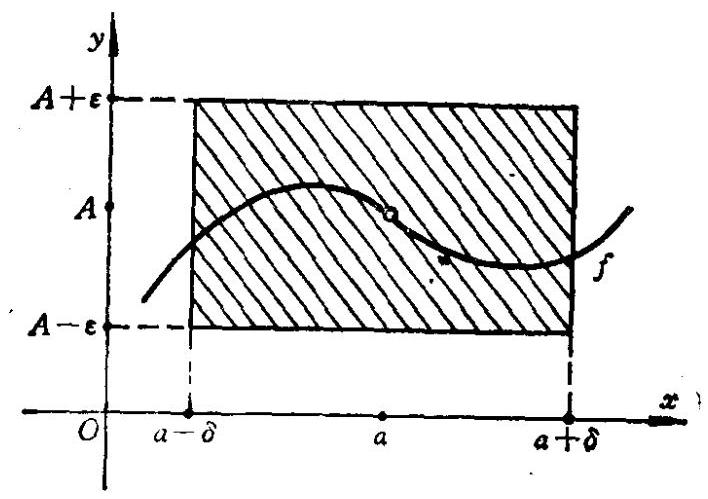
\includegraphics[max width=0.6\textwidth]{images/bo_d25ksc77aajc738obdgg_135_464_1516_708_499_0.jpg}
\end{center}
\hspace*{3em} 

图 4-1

下面我们来看几个函数极限的例子

例 1 考虑如下定义的函数 $f : \mathbf{R} - \{ 0\}  \rightarrow  \mathbf{R}$ 与函数 $g : \mathbf{R} \rightarrow  \mathbf{R}$ :
$$f\left( x\right)  = \left\{  {\begin{array}{ll} x, & \forall x > 0, \\   - x,\forall x < 0. &  \end{array}\;g\left( x\right)  = \left\{  \begin{array}{ll} x, & \forall x > 0, \\  1, & x = 0, \\   - x, & \forall x < 0. \end{array}\right. }\right.$$

\begin{center}
	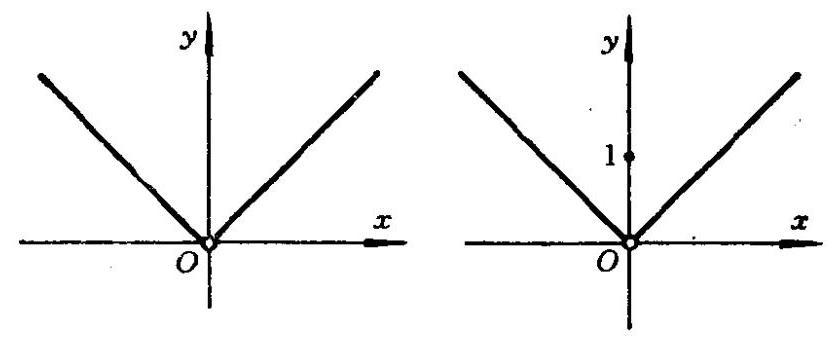
\includegraphics[max width=0.7\textwidth]{images/bo_d25ksc77aajc738obdgg_136_275_984_829_337_0.jpg}
\end{center}
\hspace*{3em} 

图 4-2

由于 $\forall x \in  \mathbf{R} - \{ 0\} ,\left| {f\left( x\right)  - 0}\right|  = \left| {g\left( x\right)  - 0}\right|  = \left| x\right|$ . 故
$$\left( {\forall \varepsilon  > 0}\right) \left( {\exists \delta  = \varepsilon  > 0}\right) \left( {\forall x \in  B\left( {0,\delta }\right) }\right)  \Rightarrow  \left\{  \begin{array}{l} \left| {f\left( x\right)  - 0}\right|  < \varepsilon , \\  \left| {g\left( x\right)  - 0}\right|  < \varepsilon . \end{array}\right.$$

因此
$$\mathop{\lim }\limits_{{x \rightarrow  0}}f\left( x\right)  = 0,\mathop{\lim }\limits_{{x \rightarrow  0}}g\left( x\right)  = 0.$$

这里 $0 \in  \mathbf{D}$ om $\left( f\right) ,0 \in  \mathbf{D}$ om(g),但 $0 \neq  g\left( 0\right)$ .

例 2 考虑函数 $x \mapsto  {x}^{p}\sin \frac{1}{x},x \in  \mathbf{R} - \{ 0\} ,\left( {p > 0}\right)$ 证明:
$$\mathop{\lim }\limits_{{x \rightarrow  0}}{x}^{p}\sin \frac{1}{x} = 0.$$

事实上, $\forall x \in  \mathbf{R} - \{ 0\}$ ,我们有
$$\left| {{x}^{p}\sin \frac{1}{x} - 0}\right|  \leq  {\left| x\right| }^{p}.$$

\begin{center}
	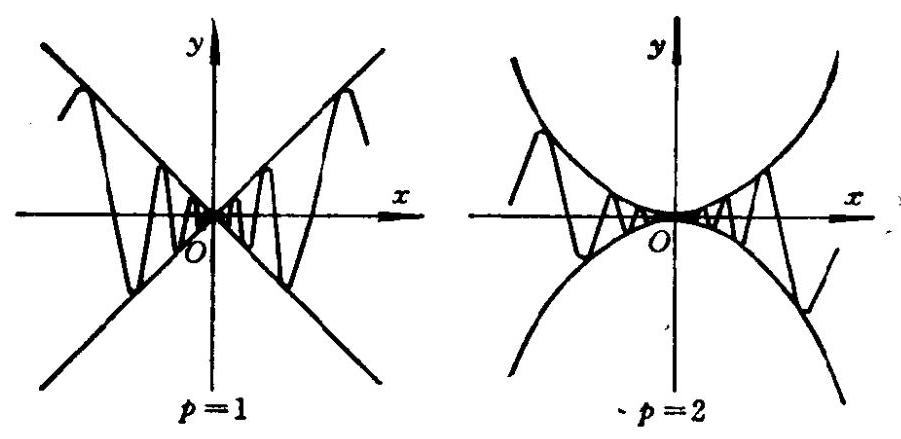
\includegraphics[max width=0.8\textwidth]{images/bo_d25ksc77aajc738obdgg_137_398_352_901_439_0.jpg}
\end{center}
\hspace*{3em} 

图 4-3

$\forall \varepsilon  > 0$ ,由 ${\left| x\right| }^{p} < \varepsilon$ 得到 $\left| x\right|  < \sqrt[p]{\varepsilon }$ ,令 $\delta  = \sqrt[p]{\varepsilon }$ ,则
$$\forall x \in  \overset{ \circ  }{B}\left( {0,\delta }\right)  \Rightarrow  \left| {{x}^{p}\sin \frac{1}{x} - 0}\right|  \leq  {\left| x\right| }^{p} < \varepsilon .$$

因此 $\mathop{\lim }\limits_{{x \rightarrow  0}}{x}^{p}\sin \frac{1}{x} = 0$ .

例3 考虑符号函数
$$x \mapsto  \operatorname{sgn}\left( x\right)  = \left\{  \begin{matrix} 1, & \forall x > 0, \\  0, & x = 0, \\   - 1, & \forall x < 0. \end{matrix}\right.$$

证明:
$$\mathop{\lim }\limits_{{x \rightarrow  0}}\operatorname{sgn}\left( x\right) \text{ 不存在, }\mathop{\lim }\limits_{{x \rightarrow  {0}^{ + }}}\operatorname{sgn}\left( x\right)  = 1,\mathop{\lim }\limits_{{x \rightarrow  {0}^{ - }}}\operatorname{sgn}\left( x\right)  =  - 1\text{ . }$$

事实上,若 $\mathop{\lim }\limits_{{x \rightarrow  0}}\operatorname{sgn}\left( x\right)  = A$ ,则
\begin{align*}
	&\left( {\forall 0 < \varepsilon  < 1}\right) \left( {\exists \delta  > 0}\right) \left( {\forall x \in  \overset{ \circ  }{B}\left( {0,\delta }\right) }\right.\\
	&\Rightarrow  \left| {\operatorname{sgn}\left( x\right)  - A}\right|  < \varepsilon\\
	&\Rightarrow  2 \leq  \left| {1 - A}\right|  + \left| {A - \left( {-1}\right) }\right|  < 2\bar{\varepsilon }\\
	&\Rightarrow  \varepsilon  > 1\text{ , }
\end{align*}

\begin{center}
	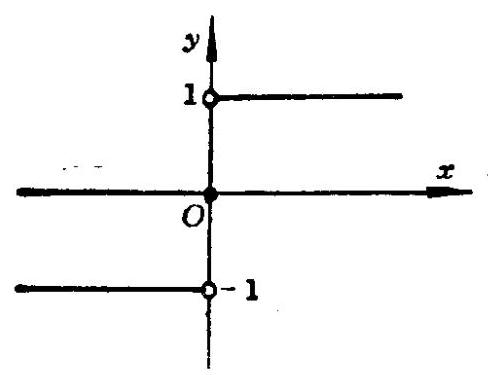
\includegraphics[max width=0.4\textwidth]{images/bo_d25ksc77aajc738obdgg_138_515_337_488_375_0.jpg}
\end{center}
\hspace*{3em} 

图 4-4

这与 $\bar{\varepsilon } < 1$ 假设相矛盾,因此 $\mathop{\lim }\limits_{{x \rightarrow  0}}\operatorname{sgn}\left( x\right)$ 不存在.

但是由于 $\forall x > 0,\operatorname{sgn}\left( x\right)  = 1;\forall x < 0,\operatorname{sgn}\left( x\right)  =  - 1$ ,故
\begin{align*}
	&\left( {\forall \varepsilon  > 0}\right) \left( {\exists \delta  = \bar{\varepsilon } > 0}\right) \left\{  \begin{array}{l} \left( {\forall x \in  {\mathring{B}}_{ + }\left( {0,\delta }\right) }\right) \\  \; \Rightarrow  \left| {\operatorname{sgn}\left( x\right)  - 1}\right|  = 0 < \varepsilon . \\  \left( {\forall x \in  {B}_{ - }\left( {0,\delta }\right) }\right)  \end{array}\right.\\
	&\Rightarrow  \left| {\operatorname{sgn}\left( x\right)  - \left( {-1}\right) }\right|  = 0 < \varepsilon \text{ . }
\end{align*}

因此 $\mathop{\lim }\limits_{{x \rightarrow  {0}^{ + }}}\operatorname{sgn}\left( x\right)  = 1,\mathop{\lim }\limits_{{x \rightarrow  {0}^{ - }}}\operatorname{sgn}\left( x\right)  =  - 1$ .

例3 实际上揭示了下面的一般结论, 即

定理 $4 \cdot  1 \cdot  1$ 设 $f : X \rightarrow  \mathbf{R}$ 是任一函数, $a \in  \mathbf{R}$ 是 $X$ 的一个双侧聚点, 那末
$$\mathop{\lim }\limits_{{x \rightarrow  a}}f\left( x\right)  = A \Leftrightarrow  \mathop{\lim }\limits_{{x \rightarrow  {a}^{ + }}}f\left( x\right)  = \mathop{\lim }\limits_{{x \rightarrow  {a}^{ - }}}f\left( x\right)  = A.$$

证明 必要性 设 $\mathop{\lim }\limits_{{x \rightarrow  a}}f\left( x\right)  = A$ . 那末由定义
$$\left( {\forall \varepsilon  > 0}\right) \left( {\exists \delta  > 0}\right) \left( {\forall x \in  X \cap  \overset{ \circ  }{B}\left( {a,\delta }\right) }\right)  \Rightarrow  \left| {f\left( x\right)  - A}\right|  < \varepsilon .$$

特别地
\begin{align*}
	&\forall x \in  X \cap  {\overset{ \circ  }{B}}_{ + }\left( {a,\delta }\right)  \Rightarrow  \left| {f\left( x\right)  - A}\right|  < \varepsilon ,\\
	&\forall x \in  X \cap  {B}_{ - }\left( {a,\delta }\right)  \Rightarrow  \left| {f\left( x\right)  - A}\right|  < \varepsilon .
\end{align*}

因此 $\mathop{\lim }\limits_{{x \rightarrow  {a}^{ + }}}f\left( x\right)  = A,\mathop{\lim }\limits_{{x \rightarrow  {a}^{ - }}}f\left( x\right)  = A$ .

充分性 设 $\mathop{\lim }\limits_{{x \rightarrow  {a}^{ + }}}f\left( x\right)  = \mathop{\lim }\limits_{{x \rightarrow  {a}^{ - }}}f\left( x\right)  = A$ ,由定义有
$$\left( {\forall \varepsilon  > 0}\right) \left\{  \begin{array}{l} \left( {\exists {\delta }_{1} > 0}\right) \left( {\forall x \in  X \cap  {\bar{B}}_{ + }\left( {a,{\delta }_{1}}\right) }\right) \\   \Rightarrow  \left| {f\left( x\right)  - A}\right|  < \varepsilon , \\  \left( {\exists {\delta }_{2} > 0}\right) \left( {\forall x \in  X \cap  {\bar{B}}_{ - }\left( {a,{\delta }_{2}}\right) }\right) \\   \Rightarrow  \left| {f\left( x\right)  - A}\right|  < \varepsilon . \end{array}\right.$$

令 $\delta  = \min \left( {{\delta }_{1},{\delta }_{2}}\right)$ ,则 $\delta  > 0$ ,并且
$$\forall x \in  X \cap  \overset{ \circ  }{B}\left( {a,\delta }\right)  \Rightarrow  \left| {f\left( x\right)  - A}\right|  < \bar{\varepsilon }.$$

因此 $\mathop{\lim }\limits_{{x \rightarrow  a}}f\left( x\right)  = A$ .

为了进一步理解函数的(a, A)型极限的定义,我们再考虑下面两个例子.

例4 考虑所谓的Dirichlet函数
$$x \mapsto  D\left( x\right)  = \left\{  \begin{array}{ll} 1, & x \in  \mathbf{Q}, \\  0, & x \in  {\mathbf{Q}}^{c}. \end{array}\right.$$

证明: $\forall a \in  \mathbf{R},\mathop{\lim }\limits_{{x \rightarrow  a}}D\left( x\right)$ 不存在.

事实上,若存在 ${a}_{0} \in  \mathbf{R}$ 使得 $\mathop{\lim }\limits_{{x \rightarrow  {a}_{0}}}D\left( x\right)  = l \in  \mathbf{R}$ ,则
$$\left( {\forall 0 < \varepsilon  < \frac{1}{2}}\right) \left( {\exists \delta  > 0}\right) \left( {\forall x \in  B\left( {{a}_{0},\delta }\right)  \Rightarrow  \left| {D\left( x\right)  - l}\right|  < \varepsilon .}\right.$$

于是特别有
\begin{align*}
	&\forall x \in  B\left( {{a}_{0},\delta }\right)  \cap  \mathbf{Q},\left| {D\left( x\right)  - l}\right|  = \left| {1 - l}\right|  < \varepsilon ,\\
	&\forall x \in  B\left( {{a}_{0},\delta }\right)  \cap  {\mathbf{Q}}^{c},\left| {D\left( x\right)  - l}\right|  = \left| {0 - l}\right|  < \varepsilon .
\end{align*}

由此推得
$$1 = \left| {1 - l + l}\right|  \leq  \left| {1 - l}\right|  + \left| l\right|  < {2\varepsilon },$$

或 $\varepsilon  > \frac{1}{2}$ ,这与 $0 < \varepsilon  < \frac{1}{2}$ 假设矛盾. 故 $\forall a \in  \mathbf{R},\mathop{\lim }\limits_{{x \rightarrow  a}}D\left( x\right)$ 不存在.

例 5 考虑如下定义的Riemann函数 $R$ :
$$R\left( x\right)  = \left\{  \begin{array}{ll} 0, & \text{ 若 }x \in  {\mathbf{Q}}^{c}, \\  1, & \text{ 若 }x = 0, \\  \frac{1}{p}, & \text{ 若 }x = \frac{q}{p},p \in  \mathbf{N},p\text{ 与 }q\text{ 互质. } \end{array}\right.$$

证明: $\forall a \in  \mathbf{R},\mathop{\lim }\limits_{{x \rightarrow  a}}R\left( x\right)  = 0$ .

为此任取 $a \in  \mathbf{R}$ .

若 $a = 0$ ; 则 $\forall \delta  > 0$ ,
$$R\left( x\right)  = \left\{  \begin{array}{ll} 0, & \forall x \in  \overset{ \circ  }{B}\left( {0,\delta }\right)  \cap  {\mathrm{Q}}^{c}, \\  \frac{1}{p}, & \forall x \in  \overset{ \circ  }{B}\left( {0,\delta }\right)  \cap  \mathrm{Q},x = \frac{q}{p},p \in  \mathbf{N},p,q\text{ 互质. } \end{array}\right.$$

若 $a \neq  0$ : 则存在 ${\delta }_{0} > 0$ 使得 $0 \in  B\left( {a,{\delta }_{0}}\right)$ ,于是
$$R\left( x\right)  = \left\{  \begin{array}{ll} 0, & \forall x \in  \overset{ \circ  }{B}\left( {a,{\delta }_{0}}\right)  \cap  {\mathbf{Q}}^{c}, \\  \frac{1}{p}, & \forall x \in  \overset{ \circ  }{B}\left( {a,{\delta }_{0}}\right)  \cap  \mathbf{Q},x = \frac{q}{p},p \in  \mathbf{N},p,q\text{ 互质. } \end{array}\right.$$

由此可知,不论 $a = 0$ 与否,
$$R\left( x\right)  = \left\{  \begin{array}{ll} 0, & \forall x \in  \overset{ \circ  }{B}\left( {a,{\delta }_{0}}\right)  \cap  {\mathrm{Q}}^{c}, \\  \frac{1}{p}, & \forall x \in  \overset{ \circ  }{B}\left( {a,{\delta }_{0}}\right)  \cap  \mathrm{Q},x = \frac{q}{p},p \in  \mathbf{N},p,q\text{ 互质 } \end{array}\right.$$

$\forall \varepsilon  > 0$ ,由 $\frac{1}{p} \geq  \varepsilon$ 知 $p \leq  \frac{1}{\varepsilon }$ . 显然在 $B\left( {a,{\delta }_{0}}\right)$ 中分母 $p \leq  \frac{1}{\varepsilon }$ 的有理数 $\frac{q}{p}$ 只有有限多个. 因此存在 $0 < \delta  < {\delta }_{0}$ ,使得在 $\overset{ \circ  }{B}\left( {a,\delta }\right)$ 中所有有理数 $\frac{q}{p}$ 的分母 $p > \frac{1}{\varepsilon }$ . 从而

$\forall x \in  \overset{ \circ  }{B}\left( {a,\delta }\right)  \cap  \mathrm{Q},x = \frac{q}{p},p \in  \mathrm{N},p,q$ 互质
$$\Rightarrow  \left| {p\left( x\right) }\right|  = \frac{1}{p} < \varepsilon \text{ . }$$

上述分析表明: $\forall \varepsilon  > 0,\exists \delta  > 0$ 使得
$$\forall x \in  B\left( {a,\delta }\right) ,\left| {\mathrm{R}\left( x\right)  - 0}\right|  < \varepsilon .$$

因此 $\mathop{\lim }\limits_{{x \rightarrow  a}}R\left( x\right)  = 0$ .

\section*{2. $\left( {\pm \infty ,A}\right)$ 型函数极限}

定义 设 $f : X \rightarrow  \mathbf{R}$ 是任一函数, $A \in  \mathbf{R}$ .

1 )设 $+ \infty$ 是 $X$ 的无穷远聚点. 我们称函数 $f$ 当 $x$ 趋于 $+ \infty$ 时极限存在并且以 $A$ 为极限,如果下述性质成立:
\begin{align*}
	&\left( {\forall \varepsilon  > 0}\right) \left( {\exists M > 0}\right) \left( {\forall x \in  X \cap  \rbrack M, + \infty \lbrack }\right)\\
	&\Rightarrow  \left| {f\left( x\right)  - A}\right|  < \varepsilon \text{ . }
\end{align*}

这时, 记为
$$\mathop{\lim }\limits_{{x \rightarrow   + \infty }}f\left( x\right)  = A\text{ 或 }f\left( x\right)  \rightarrow  A\left( {x \rightarrow   + \infty }\right) .$$

2) 设 $- \infty$ 是 $X$ 的无穷远聚点: 我们称函数 $f$ 当 $x$ 趋于 $- \infty$ 时极限存在并且以 $A$ 为极限,如果下述性质成立:
\begin{align*}
	&\left( {\forall \varepsilon  > 0}\right) \left( {\exists M > 0}\right) \left( {\forall x \in  X \cap  \rbrack  - \infty , - M\lbrack }\right)\\
	&\Rightarrow  \left| {f\left( x\right)  - A}\right|  < \varepsilon \text{ . }
\end{align*}

这时, 记为
$$\mathop{\lim }\limits_{{x \rightarrow   - \infty }}f\left( x\right)  = A\text{ 或 }f\left( x\right)  \rightarrow  A\left( {x \rightarrow   - \infty }\right) .$$

我们也可用邻域语言表述这两类极限定义.
\begin{align*}
	&\mathop{\lim }\limits_{{x \rightarrow   + \infty }}f\left( x\right)  = A \Leftrightarrow  \left( {\forall \varepsilon  > 0}\right) \left( {\exists M > 0}\right) ,f\left( {X \cap  \rbrack M, + \infty \lbrack }\right)  \subset\\
	&B\left( {A,\varepsilon }\right) \text{ , }\\
	&\mathop{\lim }\limits_{{x \rightarrow   - \infty }}f\left( x\right)  = A \Leftrightarrow  \left( {\forall \varepsilon  > 0}\right) \left( {\exists M > 0}\right) ,f\left( {X \cap  \rbrack  - \infty , - M\lbrack }\right)\\
	&\subset  B\left( {A,\varepsilon }\right) \text{ . }
\end{align*}

从几何意义上来看, $\mathop{\lim }\limits_{{x \rightarrow   + \infty }}f\left( x\right)  = A\left( {\mathop{\lim }\limits_{{x \rightarrow   + \infty }}f\left( x\right)  = A}\right)$ 表明对任意小的 $\varepsilon  > 0$ ,总可以找到一个 $M > 0$ ,使得 $f$ 在 $X \cap  \rbrack M, + \infty \lbrack (X$  $\cap  \rbrack  - \infty , - M\lbrack )$ 上的限制的图形完全位于平面 带形区域 $\rbrack M$ , $+ \infty \left\lbrack  \times \right\rbrack  A - \varepsilon ,A + \varepsilon \lbrack \left( \right)  - \infty , - M\left\lbrack  \times \right\rbrack  A - \varepsilon ,A + \varepsilon \lbrack )$ 内. (如图4-5所示)

例6 考虑函数 $x \mapsto  \frac{1}{{x}^{2}},x \in  \mathbf{R} - \{ 0\}$ . 证明:
$$\mathop{\lim }\limits_{{x \rightarrow   - \infty }}\frac{1}{{x}^{2}} = \mathop{\lim }\limits_{{x \rightarrow   - \infty }}\frac{1}{{x}^{2}} = 0.$$

\begin{center}
	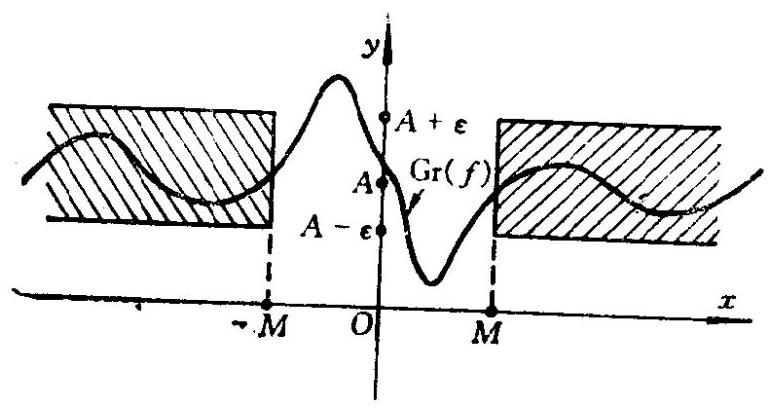
\includegraphics[max width=0.6\textwidth]{images/bo_d25ksc77aajc738obdgg_142_363_251_771_408_0.jpg}
\end{center}
\hspace*{3em} 

图 4-5

事实上, $\forall \varepsilon  > 0$ ,由 $\left| {\frac{1}{{x}^{2}} - 0}\right|  = \frac{1}{{x}^{2}} < \varepsilon$ 得到 $\left| x\right|  > \frac{1}{\sqrt{\varepsilon }}$ . 若令 $M = \frac{1}{\sqrt{\varepsilon }}$ ,则
$$\left. \begin{array}{l} \forall x \in  \rbrack M, + \infty \lbrack \\  \forall x \in  \rbrack  - \infty , - M\lbrack  \end{array}\right\}   \Rightarrow  \left| {\frac{1}{{x}^{2}} - 0}\right|  < \varepsilon .$$

因此 $\mathop{\lim }\limits_{{x \rightarrow   + \infty }}\frac{1}{{x}^{2}} = 0,\mathop{\lim }\limits_{{x \rightarrow   - \infty }}\frac{1}{{x}^{2}} = 0$ .

例 7 考虑函数 $x \mapsto  \cos \frac{1}{x},x \in  \mathbf{R} - \{ 0\}$ . 证明:
$$\mathop{\lim }\limits_{{x \rightarrow   + \infty }}\cos \frac{1}{x} = \mathop{\lim }\limits_{{x \rightarrow   - \infty }}\cos \frac{1}{x} = 1$$

事实上,由于 $\forall x \in  \mathbf{R},\left| {\sin x}\right|  \leq  \left| x\right|$ ,故 $\forall x \in  \mathbf{R} - \{ 0\}$ ,
$$\left| {\cos \frac{1}{x} - 1}\right|  = \left| {2{\sin }^{2}\frac{1}{2x}}\right|  \leq  2 \cdot  \frac{1}{4{x}^{2}} = \frac{1}{2{x}^{2}}.$$

因此, $\forall \varepsilon  > 0$ ,由 $\frac{1}{2{x}^{2}} < \varepsilon$ 得到 $\left| x\right|  > \frac{1}{\sqrt{2\varepsilon }}$ . 若令 $M = \frac{1}{\sqrt{2\varepsilon }}$ ,则
$$\forall x \in  \rbrack M, + \infty \left\lbrack  \;\right\rbrack   \Rightarrow  \left| {\cos \frac{1}{x} - 1}\right|  < \varepsilon .$$

因此 $\mathop{\lim }\limits_{{x \rightarrow   + \infty }}\cos \frac{1}{x} = 1,\mathop{\lim }\limits_{{x \rightarrow   - \infty }}\cos \frac{1}{x} = 1$ .

例 8 考虑函数 $x \mapsto  \frac{{x}^{2} - 1}{2\left( {{x}^{2} + x - 2}\right) },x \in  \mathbf{R} - \{ 1, - 2\}$ . 证明:
$$\mathop{\lim }\limits_{{x \rightarrow   + \infty }}\frac{{x}^{2} - 1}{2\left( {{x}^{2} + x - 2}\right) } = \mathop{\lim }\limits_{{x \rightarrow   - \infty }}\frac{{x}^{2} - 1}{2\left( {{x}^{2} + x - 2}\right) } = \frac{1}{2}.$$

事实上,由于 $\forall x \neq  1, - 2$ ,我们有
$$\left| {\frac{{x}^{2} - 1}{2\left( {{x}^{2} + x - 2}\right) } - \frac{1}{2}}\right|  = \left| \frac{-2\left( {x - 1}\right) }{2\left( {x - 1}\right) \left( {x + 2}\right) }\right|  = \frac{1}{\left| x + 2\right| }.$$

故若首先限制 $\left| x\right|  > 2$ ,则 $\forall \varepsilon  > 0$ ,由 $\frac{1}{\left| x + 2\right| } \leq  \frac{1}{\left| x\right|  - 2} < \varepsilon$ 得到 $\left| x\right|  > 2 + \frac{1}{\varepsilon }$ . 令 $M = 2 + \frac{1}{\varepsilon }$ ,则
$$\left. {\forall x \in  \rbrack M, + \infty \lbrack }\right\}   \Rightarrow  \left| {\frac{{x}^{2} - 1}{2\left( {{x}^{2} + x - 2}\right) } - \frac{1}{2}}\right|  < \bar{\varepsilon }.$$

因此 $\mathop{\lim }\limits_{{x \rightarrow   + \infty }}\frac{{x}^{2} - 1}{2\left( {{x}^{2} + x - 2}\right) } = \frac{1}{2},\mathop{\lim }\limits_{{x \rightarrow   - \infty }}\frac{{x}^{2} - 1}{2\left( {{x}^{2} + x - 2}\right) } = \frac{1}{2}$ .

例 9 考虑函数 $x \mapsto  \sin x,x \in  \mathbf{R}$ . 证明 $\mathop{\lim }\limits_{{x \rightarrow   + \infty }}\sin x$ 不存在.

事实上,如果存在 $A \in  \mathbf{R}$ 使得 $\mathop{\lim }\limits_{{x \rightarrow   + \infty }}\sin x = A$ ,则
\begin{align*}
	&\left( {\forall 0 < \varepsilon  < 1}\right) \left( {\exists M > 0}\right) \left( {\forall x \in  \rbrack M, + \infty \lbrack }\right)\\
	&\Rightarrow  \left| {\sin x - A}\right|  < \varepsilon \text{ . }
\end{align*}

于是对 $n$ 充分大, ${2n\pi } - \frac{\pi }{2},{2n\pi } + \frac{\pi }{2} > M$ . 从而
\begin{align*}
	&\left| {\sin \left( {{2n\pi } - \frac{\pi }{2}}\right)  - A}\right|  = \left| {\left( {-1}\right)  - A}\right|  < \bar{\varepsilon },\\
	&\left| {\sin \left( {{2n\pi } + \frac{\pi }{2}}\right)  - A}\right|  = \left| {1 - A}\right|  < \varepsilon .
\end{align*}

由此推得
\begin{align*}
	&2 = \left| {1 - \left( {-1}\right) }\right|  = \left| {1 - A + A - \left( {-1}\right) }\right|\\
	&\leq  \left| {1 - A}\right|  + \left| {A - \left( {-1}\right) }\right|  < 2\bar{\varepsilon }.
\end{align*}

于是 $\varepsilon  > 1$ ,这与 $0 < \varepsilon  < 1$ 假设相矛盾. 因此 $\mathop{\lim }\limits_{{x \rightarrow   + \infty }}\sin x$ 不存在.

\section*{习 题}

1. 用极限定义证明下列各极限:

1) $\mathop{\lim }\limits_{{x \rightarrow  0}}x\sin \frac{1}{x} = 0$ , 2) $\mathop{\lim }\limits_{{x \rightarrow  a}}\sqrt[n]{x} = \sqrt[n]{a}\;\left( {a > 0,n \in  \mathbf{N}}\right)$ ,

3) $\mathop{\lim }\limits_{{x \rightarrow  1}}\left( {3{x}^{3} - 2}\right)  = 1$ , 4) $\mathop{\lim }\limits_{{x \rightarrow  3}}\left( {2{x}^{2} - x}\right)  = {15}$ ,

5) $\mathop{\lim }\limits_{{x \rightarrow   \pm  \infty }}\frac{\left\lbrack  x\right\rbrack  }{x} = 1$ , 6) $\mathop{\lim }\limits_{{x \rightarrow   \pm  \infty }}\frac{2{x}^{2} - 1}{3{x}^{2} - x} = \frac{2}{3}$ ,

7) $\mathop{\lim }\limits_{{x \rightarrow   \pm  \infty }}\frac{3{x}^{2} - 1}{{x}^{2} + x + 1} = 3$ , 8) $\mathop{\lim }\limits_{{x \rightarrow   \pm  \infty }}\left( {\sqrt{{x}^{2} + x} - x}\right)  = \frac{1}{2}$ .

2. 证明: 极限 $\mathop{\lim }\limits_{{x \rightarrow  0}}\frac{1}{x}$ 不存在.

3. 证明: 若 $\mathop{\lim }\limits_{{x \rightarrow  a}}f\left( x\right)  = A$ ,则 $\mathop{\lim }\limits_{{x \rightarrow  a}}\left| {f\left( x\right) }\right|  = \left| A\right|$ ,这里 $a \in  R$ 或 $a =$  $\pm  \infty$ .

4. 设函数 $x \mapsto  x - \left\lbrack  x\right\rbrack  ,x \in  R$ .

1) 证明: $\forall n \in  \mathbf{Z},\mathop{\lim }\limits_{{x \rightarrow  n}}\left( {x - \left\lbrack  x\right\rbrack  }\right)$ 不存在;

2) 证明: $\forall a \in  \mathbf{Z},\mathop{\lim }\limits_{{x \rightarrow  a}}\left( {x - \left\lbrack  x\right\rbrack  }\right)$ 存在.

5. 设 $f : R \rightarrow  R$ 是以 $T$ 为周期的周期函数.

证明: 若 $\mathop{\lim }\limits_{{x \rightarrow   + \infty }}f\left( x\right)  = A$ ,则 $f\left( x\right)  \equiv  A,\forall x \in  R$ .

6. 对函数
$$x \mapsto  f\left( x\right)  = \left\{  \begin{array}{l} x,\text{ 若 }x \in  \mathbf{Q} \\   - x\text{ 若 }x \in  {\mathbf{Q}}^{2}, \end{array}\right.$$

证明: $\mathop{\lim }\limits_{{x \rightarrow  0}}f\left( x\right)  = 0,\forall a \neq  0,\mathop{\lim }\limits_{{x \rightarrow  a}}f\left( x\right)$ 不存在.

7. 设 $\left\lbrack  {a,b}\right\rbrack$ 是任一有限闭区间. 假设 $\forall {x}_{0} \in  \left\lbrack  {a,b}\right\rbrack$ ,极限 $\mathop{\lim }\limits_{{x \rightarrow  {x}_{0}}}f\left( x\right)$ 存在. 试用两 种不同的方法证明: 存在 $M > 0$ ,使得 $\forall x \in  \left\lbrack  {a,b}\right\rbrack  ,\left| {f\left( x\right) }\right|  \leq$  $M$ .

8. 设 ${P}_{n}\left( x\right)  = {a}_{n}{x}^{n} + {a}_{n - 1}{x}^{n - 1} + \cdots  + {a}_{1}x + {a}_{0}$ ,其中 $n \geq  1,{a}_{n} \neq  0$ . 试用极限定义证明 $\mathop{\lim }\limits_{{x \rightarrow   \pm  \infty }}\left| {{P}_{n}\left( x\right) }\right|  =  + \infty$ .

\section{函数极限的性质}

函数极限的性质与收敛序列极限的大多数性质是类似的. 这里我们只对(a, A)型的函数极限性质进行叙述和证明. 对于 $\left( {\pm \infty ,A}\right)$ 型的情形,读者可仿照(a, A)型的性质自己去论述.

\section*{1. 函数极限的一般性质}

性质 1 如果函数 $f : X \rightarrow  \mathbf{R}$ 当 $x \rightarrow  a$ 时有极限存在,则极限是唯一的.

证明 设 $\mathop{\lim }\limits_{{x \rightarrow  a}}f\left( x\right)  = A,\mathop{\lim }\limits_{{x \rightarrow  a}}f\left( x\right)  = {A}^{\prime }$ 并且 $A \neq  {A}^{\prime }$ . 那末由 $\mathbf{R}$ 的Hausdorff分离性知,存在 ${\varepsilon }_{0} > 0$ 使得
$$B\left( {A,{\varepsilon }_{0}}\right)  \cap  B\left( {{A}^{\prime },{\varepsilon }_{0}}\right)  = \varnothing .$$

另一方面,对于 ${\varepsilon }_{0} > 0$ ,存在 ${\delta }_{1} > 0,{\delta }_{2} > 0$ 使得
\begin{align*}
	&f\left( {X \cap  \overset{ \circ  }{B}\left( {a,{\delta }_{1}}\right) }\right)  \subset  B\left( {A,{\varepsilon }_{0}}\right) ,\\
	&f\left( {X \cap  \overset{ \circ  }{B}\left( {a,{\delta }_{2}}\right) }\right)  \subset  B\left( {{A}^{\prime },{\varepsilon }_{0}}\right) .
\end{align*}

令 $\delta  = \min \left( {{\delta }_{1},{\delta }_{2}}\right)$ ,则 $\delta  > 0$ ,并且
$$f\left( {X \cap  B\left( {a,\delta }\right) }\right)  \subset  B\left( {A,{\varepsilon }_{0}}\right)  \cap  B\left( {{A}^{\prime },{\varepsilon }_{0}}\right) .$$

于是 $f\left( {X \cap  B\left( {a,\delta }\right) }\right)  = \varnothing$ ,这与 $a$ 为 $X$ 的聚点相矛盾,因此 $A =$  ${A}^{\prime }$ .

性质 2 若 $\mathop{\lim }\limits_{{x \rightarrow  a}}f\left( x\right)  = A$ ,则 $f$ 在 $a$ 处是局部有界的. 即
$$\left( {\exists M > 0}\right) \left( {\exists \delta  > 0}\right) \left( {\forall x \in  X \cap  B\left( {a,\delta }\right) }\right)  \Rightarrow  \left| {f\left( x\right) }\right|  \leq  M.$$

证明 因为 $\mathop{\lim }\limits_{{x \rightarrow  a}}f\left( x\right)  = A$ ,所以由定义,对 $\varepsilon  = 1 > 0$ ,存在 $\delta  > 0$ ,使得
\begin{align*}
	&\forall x \in  X \cap  \overset{ \circ  }{B}\left( {a,\delta }\right)  \Rightarrow  \left| {f\left( x\right)  - A}\right|  < 1\\
	&\Rightarrow  \left| {f\left( x\right) }\right|  \leq  \left| A\right|  + \left| {f\left( x\right)  - A}\right|\\
	&< \left| A\right|  + 1\text{ . }
\end{align*}

取 $M = 1 + \left| A\right|$ 即可.

性质 3 (Cauchy收敛准则) 函数 $f : X \rightarrow  \mathbf{R}$ 当 $x$ 趋于 $a$ 时极限存在的充分必要条件是:
$$\left( {\forall \varepsilon  > 0}\right) \left( {\exists \delta  > 0}\right) \left( {\forall x,{x}^{\prime } \in  X \cap  \overset{ \circ  }{B}\left( {a,\delta }\right) }\right)  \Rightarrow   \mid  f\left( x\right)$$

$- f\left( {x}^{\prime }\right)  \mid   < \varepsilon .$ 证明 必要性 设 $\mathop{\lim }\limits_{{x \rightarrow  a}}f\left( x\right)  = A$ . 由定义有
\begin{align*}
	&\left( {\forall \varepsilon  > 0}\right) \left( {\exists \delta  > 0}\right) \left( {\forall x,{x}^{\prime } \in  X \cap  \overset{ \circ  }{B}\left( {a,\delta }\right) }\right)\\
	&\Rightarrow  \left| {f\left( x\right)  - A}\right|  < \varepsilon /2,\left| {f\left( {x}^{\prime }\right)  - A}\right|  < \varepsilon /2\\
	&\Rightarrow  \left| {f\left( x\right)  - f\left( {x}^{\prime }\right) }\right|  \leq  \left| {f\left( x\right)  - A}\right|  + \left| {A - f\left( {x}^{\prime }\right) }\right|\\
	&< \varepsilon /2 + \varepsilon /2 = \varepsilon .
\end{align*}

充分性 假设条件满足, 即
\begin{align*}
	&\left( {\forall \varepsilon  > 0}\right) \left( {\exists \delta  > 0}\right) \left( {\forall x,{x}^{\prime } \in  X \cap  \overset{ \circ  }{B}\left( {a,\delta }\right) }\right)\\
	&\Rightarrow  \left| {f\left( x\right)  - f\left( {x}^{\prime }\right) }\right|  < \varepsilon .
\end{align*}

证明分两步进行. ${1}^{ \circ  }$ 证明: 存在一个收敛的实数序列 $\left\langle  {f\left( {x}_{n}\right) }\right\rangle$ . 因为 $a \in  \mathbf{R}$ 是 $X$ 的聚点,所以 $\forall n \in  \mathbf{N},X \cap  \overset{ \circ  }{B}\left( {a,\frac{1}{n}}\right)  \neq  \varnothing$ . 任取 ${x}_{n} \in  X \cap  \overset{ \circ  }{B}\left( {a,\frac{1}{n}}\right) \left( {n \in  \mathbf{N}}\right)$ . 于是我们得到一实数序列 $\left\langle  {f\left( {x}_{n}\right) }\right\rangle$ .

由于 $\mathop{\lim }\limits_{{n \rightarrow   + \infty }}\frac{1}{n} = 0$ ,故对 $\delta  > 0$ 存在 $N \in  \mathbf{N}$ 使得
$$\forall n,m \in  \mathbf{N},n,m \geq  \mathbf{N} \Rightarrow  \frac{1}{n} \leq  \frac{1}{N} < \delta ,\frac{1}{m} \leq  \frac{1}{N} < \delta .$$

于是
\begin{align*}
	&\forall n,m \in  N,n,m \geq  N \Rightarrow  {x}_{n},{x}_{m} \in  X \cap  \overset{ \circ  }{B}\left( {a,\frac{1}{N}}\right)\\
	&\subset  X \cap  \overset{ \circ  }{B}\left( {a,\delta }\right)\\
	&\Rightarrow  \left| {f\left( {x}_{n}\right)  - f\left( {x}_{m}\right) }\right|  < \varepsilon .
\end{align*}

此即表明 $\left\langle  {f\left( {x}_{n}\right) }\right\rangle$ 是 Cauchy 实数序列. 由 $\mathbf{R}$ 的完备性知 $\left\langle  {f\left( {x}_{n}\right) }\right\rangle$ 收敛,令 $\mathop{\lim }\limits_{{n \rightarrow   + \infty }}f\left( {x}_{n}\right)  = A$ .

${2}^{ \circ  }$ . 证明: $\mathop{\lim }\limits_{{x \rightarrow  a}}f\left( x\right)  = A$ .

因为 $\mathop{\lim }\limits_{{n \rightarrow   + \infty }}f\left( {x}_{n}\right)  = A$ ,所以由定义
$$\left( {\forall \varepsilon  > 0}\right) \left( {\exists N \in  \mathbf{N}}\right) \left( {\forall n \in  \mathbf{N},n \geq  N}\right)  \Rightarrow  \left| {f\left( {x}_{n}\right)  - A}\right|  < \varepsilon .$$

于是由已知条件及 $\forall n \in  \mathbf{N},n \geq  N,{x}_{n} \in  X \cap  B\left( {a,\delta }\right)$ 知,
\begin{align*}
	&\forall x \in  X \cap  \overset{ \circ  }{B}\left( {a,\delta }\right)  \Rightarrow  \left| {f\left( x\right)  - f\left( {x}_{n}\right) }\right|  < \varepsilon\\
	&\Rightarrow  \left| {f\left( x\right)  - A}\right|  \leq  \left| {f\left( x\right)  - f\left( {x}_{n}\right) }\right|\\
	&+ \left| {f\left( {x}_{n}\right)  - A}\right|  < \varepsilon  + \varepsilon  = {2\varepsilon }.
\end{align*}

因此 $\mathop{\lim }\limits_{{x \rightarrow  a}}f\left( x\right)  = A$ .

反映函数极限与序列极限之间联系的是下面的重要定理.

性质 4 (Heine定理) 函数 $f : X \rightarrow  \mathbf{R}$ 当 $x$ 趋于 $a$ 时有极限 $A$ 的充分必要条件是:
$$\forall {x}_{n} \in  X - \{ a\} \left( {n \in  \mathbf{N}}\right) \text{ 且 }{x}_{n} \rightarrow  a\left( {n \rightarrow   + \infty }\right) ,\mathop{\lim }\limits_{{n \rightarrow   + \infty }}f\left( {x}_{n}\right)  = A.$$

证明 必要性 设 $\mathop{\lim }\limits_{{x \rightarrow  a}}f\left( x\right)  = A.{x}_{n} \in  X - \{ a\}$ ,并且 ${x}_{n} \rightarrow  a$  $\left( {n \rightarrow   + \infty }\right)$ . 由定义
\begin{align*}
	&\left( {\forall \varepsilon  > 0}\right) \left( {\exists \delta  > 0}\right) \left( {\forall x \in  X \cap  B\left( {a,\delta }\right) }\right)  \Rightarrow  \left| {f\left( x\right)  - A}\right|  < \varepsilon .\\
	&\text{ (对 }\delta  > 0\text{ ) }\left( {\exists N \in  \mathbf{N}}\right) \left( {\forall n \in  \mathbf{N},n \geq  N}\right)  \Rightarrow  {x}_{n} \in  B\left( {a,\delta }\right) \text{ . }
\end{align*}

从而
$$\forall n \in  \mathbf{N},n \geq  N \Rightarrow  \left| {f\left( {x}_{n}\right)  - A}\right|  < \varepsilon .$$

因此 $\mathop{\lim }\limits_{{n \rightarrow  \infty }}f\left( {x}_{n}\right)  = A$ .

充分性 假设条件成立, 即
$$\forall {x}_{n} \in  X - \{ a\} \left( {n \in  \mathbf{N}}\right) ,{x}_{n} \rightarrow  a\left( {n \rightarrow   + \infty }\right) \text{ ,则 }\mathop{\lim }\limits_{{n \rightarrow   + \infty }}f\left( {x}_{n}\right)  = A\text{ . }$$

我们用反证法证明. 假设 $\mathop{\lim }\limits_{{x \rightarrow  a}}f\left( x\right)  = A$ ,则
\begin{align*}
	&\left( {\exists {\varepsilon }_{0} > 0}\right) \left( {\forall n \in  \mathbf{N}}\right) \left( {\exists {x}_{n} \in  X \cap  \overset{ \circ  }{B}\left( {a,\frac{1}{n}}\right) }\right)\\
	&\Rightarrow  \left| {f\left( {x}_{n}\right)  - A}\right|  \geq  {\varepsilon }_{0}
\end{align*}
(*)

由此得一实数序列 $\left\langle  {x}_{n}\right\rangle$ ,它满足: ${x}_{n} \in  X - \{ a\} ,{x}_{n} \rightarrow  a\left( {n \rightarrow   + \infty }\right)$ . 于是 $\mathop{\lim }\limits_{{n \rightarrow   + \infty }}f\left( {x}_{n}\right)  = A$ ,在 (*) 式中令 $n \rightarrow   + \infty$ 得到 ${\varepsilon }_{0} \leq  0$ . 这与 ${\varepsilon }_{0} > 0$ 矛盾,故必有 $\mathop{\lim }\limits_{{x \rightarrow  a}}f\left( x\right)  = A$ .

例 1 考虑函数 $x \mapsto  \sin \frac{1}{x},x \in  \mathbf{R} - \{ 0\}$ 及
$$x \mapsto  \sin x,x \in  \mathbf{R}.$$

利用Heine定理证明:

1) $\mathop{\lim }\limits_{{x \rightarrow  0}}\sin \frac{1}{x}$ 不存在,2) $\mathop{\lim }\limits_{{x \rightarrow   \pm  \infty }}\sin x$ 不存在.

为此,1) 取 ${x}_{n} = \frac{1}{2n\pi },{x}_{n}^{\prime } = \frac{1}{{2n\pi } + \frac{\pi }{2}}\left( {n \in  \mathbf{N}}\right)$ . 则 ${x}_{n},{x}_{n}^{\prime } \in  \mathbf{R} - \{ 0\} \left( {\forall n \in  \mathbf{N}}\right)$ ,并且 ${x}_{n} \rightarrow  0,{x}_{n}^{\prime } \rightarrow  0\left( {n \rightarrow   + \infty }\right)$ 但是
$$\mathop{\lim }\limits_{{n \rightarrow   + \infty }}\sin \frac{1}{{x}_{n}} = 0,\mathop{\lim }\limits_{{n \rightarrow   + \infty }}\sin \frac{1}{{x}_{n}^{\prime }} = 1.$$

因此由 Heine 定理知, $\mathop{\lim }\limits_{{x \rightarrow  0}}\sin \frac{1}{x}$ 不存在.

2) 取 ${x}_{n} = {2n\pi },{x}_{n}^{\prime } = {2n\pi } + \frac{\pi }{2}\left( {n \in  \mathbf{N}}\right)$ ,则 ${x}_{n} \rightarrow   + \infty$ ,

${x}_{n}^{\prime } \rightarrow   + \infty \left( {n \rightarrow   + \infty }\right)$ . 由于
$$\sin {x}_{n} = 0,\;\sin {x}_{n}^{\prime } = 1,$$

故由Heine定理知, $\mathop{\lim }\limits_{{x \rightarrow   + \infty }}\sin x$ 不存在.

函数 $x \mapsto  \sin \frac{1}{x},x \in  \mathbf{R} - \{ 0\}$ 的图形如图 4-6 所示.

例 2 考虑函数 $x \mapsto  x - \left\lbrack  x\right\rbrack  ,x \in  \mathbf{R}$ (因此 $x - \left\lbrack  x\right\rbrack$ 是 $x$ 的小数部分),证明 $\mathop{\lim }\limits_{{x \rightarrow   \pm  \infty }}x - \left\lbrack  x\right\rbrack$ 不存在.

\begin{center}
	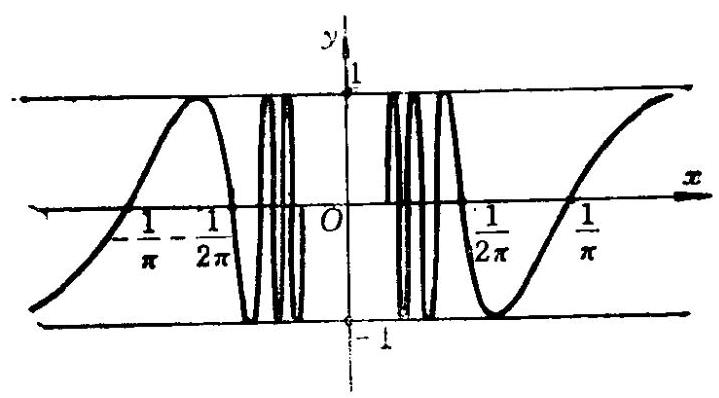
\includegraphics[max width=0.6\textwidth]{images/bo_d25ksc77aajc738obdgg_149_439_300_719_398_0.jpg}
\end{center}
\hspace*{3em} 

图 4-6

为此取 ${x}_{n} = n,{x}_{n}^{\prime } = n + \frac{1}{2}\left( {n \in  \mathbf{N}}\right)$ ,则 ${x}_{n} \rightarrow   + \infty ,{x}_{n}^{\prime } \rightarrow   + \infty$

$\left( {n \rightarrow   + \infty }\right)$ . 由于
$${x}_{n} - \left\lbrack  {x}_{n}\right\rbrack   = 0,{x}_{n}^{\prime } - \left\lbrack  {x}_{n}^{\prime }\right\rbrack   = \frac{1}{2}\left( {\forall n \in  \mathbf{N}}\right) ,$$

故
$$\mathop{\lim }\limits_{{n \rightarrow   + \infty }}\left( {{x}_{n} - \left\lbrack  {x}_{n}\right\rbrack  }\right)  = 0,\mathop{\lim }\limits_{{n \rightarrow   + \infty }}\left( {{x}_{n}^{\prime } - \left\lbrack  {x}_{n}^{\prime }\right\rbrack  }\right)  = \frac{1}{2}.$$

由Heine定理知, $\mathop{\lim }\limits_{{x \rightarrow   + \infty }}x - \left\lbrack  x\right\rbrack$ 不存在.

同理可证 $\mathop{\lim }\limits_{{x \rightarrow   - \infty }}x - \left\lbrack  x\right\rbrack$ 也不存在.

函数 $x \mapsto  x - \left\lbrack  x\right\rbrack  ,x \in  \mathbf{R}$ 的图形如图 4-7 所示.

\begin{center}
	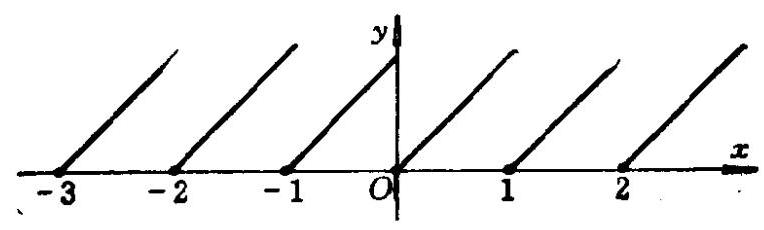
\includegraphics[max width=0.6\textwidth]{images/bo_d25ksc77aajc738obdgg_149_391_1544_764_230_0.jpg}
\end{center}
\hspace*{3em} 

图 4-7

\section*{2. 函数极限的不等式性质}

性质 5 若 $\mathop{\lim }\limits_{{x \rightarrow  a}}f\left( x\right)  = A > r\left( { < r}\right)$ ,则
$$\left( {\exists \delta  > 0}\right) \left( {\forall x \in  X \cap  \overset{ \circ  }{B}\left( {a,\delta }\right) }\right)  \Rightarrow  f\left( x\right)  > r\left( { < r}\right) .$$

证明 我们只对 $A > r$ 的情形证明. 由于 $\mathop{\lim }\limits_{{x \rightarrow  a}}f\left( x\right)  = A > r$ ,故对 $\varepsilon  = \frac{A - r}{2} > 0$ ,存在 $\delta  > 0$ 使得
\begin{align*}
	&\forall x \in  X \cap  \overset{ \circ  }{B}\left( {a,\delta }\right)  \Rightarrow  \left| {f\left( x\right)  - A}\right|  < \frac{A - r}{2}\\
	&\Rightarrow  f\left( x\right)  > A - \frac{A - r}{2} = \frac{A + r}{2} > r\text{ . }
\end{align*}

性质 6 设 $f,g$ 是任意两个函数,
$$X = \operatorname{Dom}\left( f\right)  \cap  \operatorname{Dom}\left( g\right)  \neq  \varnothing ,$$

$a \in  \mathbf{R}$ 是 $X$ 的聚点,并且

1) $\mathop{\lim }\limits_{{x \rightarrow  a}}f\left( x\right)  = A,\mathop{\lim }\limits_{{x \rightarrow  a}}g\left( x\right)  = B$ ;

2) $A > B\left( {A < B}\right)$ ,

划

$\left( {\exists \delta  > 0}\right) \left( {\forall x \in  X \cap  \overset{ \circ  }{B}\left( {a,\delta }\right) }\right)  \Rightarrow  f\left( x\right)  > g\left( x\right)$
$$\left( {f\left( x\right)  < g\left( x\right) }\right) \text{ . }$$

证明 我们只对 $A > B$ 的情形证明. 令 $r = \frac{A + B}{2}$ ,则由 $\mathop{\lim }\limits_{{x \rightarrow  a}}f\left( x\right)  = A > r > B = \mathop{\lim }\limits_{{x \rightarrow  a}}g\left( x\right)$ 及性质 5 知
\begin{align*}
	&\left( {\exists {\delta }_{1} > 0}\right) \left( {\forall x \in  X \cap  \overset{ \circ  }{B}\left( {a,{\delta }_{1}}\right) }\right)  \Rightarrow  f\left( x\right)  > r,\\
	&\left( {\exists {\delta }_{2} > 0}\right) \left( {\forall x \in  X \cap  \overset{ \circ  }{B}\left( {a,{\delta }_{2}}\right) }\right)  \Rightarrow  g\left( x\right)  < r.
\end{align*}

令 $\delta  = \min \left( {{\delta }_{1},{\delta }_{2}}\right)$ ,则
$$\forall x \in  X \cap  B\left( {a,\delta }\right)  \Rightarrow  f\left( x\right)  > g\left( x\right) .$$

性质 7 设 $f,g$ 是任意两个函数,
$$X = \operatorname{Dom}\left( f\right)  \cap  \operatorname{Dom}\left( g\right)  \neq  \varnothing ,$$

$a \in  \mathbf{R}$ 是 $X$ 的聚点,并且

1) $\mathop{\lim }\limits_{{x \rightarrow  a}}f\left( x\right)  = A,\mathop{\lim }\limits_{{x \rightarrow  a}}g\left( x\right)  = B$ ;

2) $\left( {\exists \delta  > 0}\right) \left( {\forall x \in  X \cap  \overset{ \circ  }{B}\left( {a,\delta }\right) }\right)  \Rightarrow  f\left( x\right)  \geq  g\left( x\right) (f\left( x\right)  \leq$

$g\left( x\right) )$ ,

则
$$A \geq  B\left( {A \leq  B}\right) \text{ . }$$

证明 用反证法, 由性质 6 立即推出.

附注 在条件 2 )中即使把 $f\left( x\right)  \geq  g\left( x\right) \left( {f\left( x\right)  \leq  g\left( x\right) }\right)$ 换成严格不等式 $f\left( x\right)  > g\left( x\right) \left( {f\left( x\right)  < g\left( x\right) }\right)$ ,也不一定有 $A > B(A <$  $B)$ . 例如函数
$$x \mapsto  2{x}^{2},x \in  \mathbf{R} - \{ 0\} \text{ 与 }x \mapsto  {x}^{2},x \in  \mathbf{R} - \{ 0\} ,$$

显然有 $2{x}^{2} > {x}^{2}\left( {\forall x \in  \mathbf{R}-\{ 0\} }\right)$ ,但 $\mathop{\lim }\limits_{{x \rightarrow  0}}2{x}^{2} = \mathop{\lim }\limits_{{x \rightarrow  0}}{x}^{2} = 0$ .

性质 8 设 $f,g,h$ 是任意三个函数,
$$X = \operatorname{Dom}\left( f\right)  \cap  \operatorname{Dom}\left( g\right)  \cap  \operatorname{Dom}\left( h\right)  \neq  \varnothing ,$$

$a \in  \mathbf{R}$ 是 $X$ 的聚点,并且

1) $\left( {\exists \delta  > 0}\right) \left( {\forall x \in  X \cap  \overset{ \circ  }{B}\left( {a,\delta }\right) }\right)  \Rightarrow  f\left( x\right)  \leq  h\left( x\right)  \leq  g\left( x\right)$ ,

2) $\mathop{\lim }\limits_{{x \rightarrow  a}}f\left( x\right)  = \mathop{\lim }\limits_{{x \rightarrow  a}}g\left( x\right)  = A$ ,

则
$$\mathop{\lim }\limits_{{x \rightarrow  a}}h\left( x\right)  = A$$

证明 因为 $\mathop{\lim }\limits_{{x \rightarrow  a}}f\left( x\right)  = \mathop{\lim }\limits_{{x \rightarrow  a}}g\left( x\right)  = A$ ,所以由定义
\begin{align*}
	&\left( {\forall \varepsilon  > 0}\right) \left( {\exists {\delta }^{\prime } > 0}\right) \left( {\forall x \in  X \cap  \overset{ \circ  }{B}\left( {a,\delta }\right) }\right)\\
	&\Rightarrow  \left| {f\left( x\right)  - A}\right|  < \varepsilon ,\left| {g\left( x\right)  - A}\right|  < \varepsilon\\
	&\Rightarrow  A - \varepsilon  < f\left( x\right) ,g\left( x\right)  < A + \varepsilon .
\end{align*}

令 $\eta  = \min \left( {\delta ,{\delta }^{\prime }}\right)$ ,则由上述不等式及条件 1 )推得
\begin{align*}
	&\forall x \in  X \cap  \overset{ \circ  }{B}\left( {a,\eta }\right)  \Rightarrow  A - \varepsilon  < h\left( x\right)  < A + \varepsilon\\
	&\Rightarrow  \left| {h\left( x\right)  - A}\right|  < \varepsilon \text{ . }
\end{align*}

因此 $\mathop{\lim }\limits_{{x \rightarrow  a}}h\left( x\right)  = A$ .

例 3 证明: $\mathop{\lim }\limits_{{x \rightarrow  0}}\frac{\sin x}{x} = 1$ .

首先设 $0 < x < \frac{\pi }{2}$ . 如图 4-8 所示, $A\text{ 、 }B$ 是单位圆周上两点,

使得
$$\angle {AOB} = x\text{ . }$$

\begin{center}
	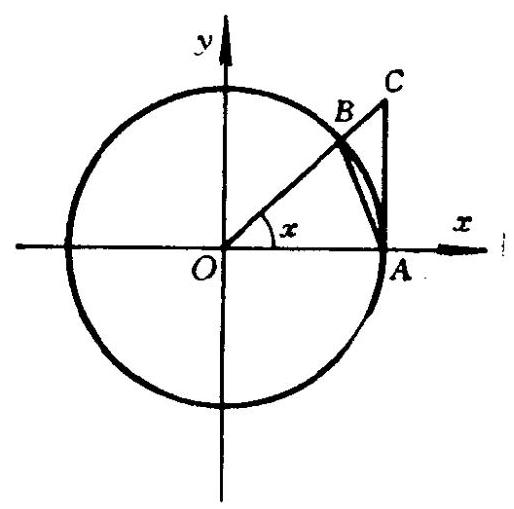
\includegraphics[max width=0.4\textwidth]{images/bo_d25ksc77aajc738obdgg_152_475_505_514_509_0.jpg}
\end{center}
\hspace*{3em} 

图 4-8

则由图形可知

三角形 ${AOB}$ 的面积 ${S}_{1} = \frac{1}{2} \cdot  1 \cdot  \sin x$ ,

扇形 ${AOB}$ 的面积 ${S}_{2} = \frac{1}{2} \cdot  1 \cdot  x$ ,

三角形 ${AOC}$ 的面积 ${S}_{3} = \frac{1}{2} \cdot  1 \cdot  \operatorname{tg}x$ ,

并且 ${S}_{1} < {S}_{2} < {S}_{3}$ . 由此得到不等式
$$\sin x < x < \operatorname{tg}x.$$

两边同除以 $\sin x \neq  0$ ,得 $1 < \frac{x}{\sin x} < \frac{1}{\cos x}$ 或
$$\cos x < \frac{\sin x}{x} < 1\left( {0 < x < \frac{\pi }{2}}\right) .$$

现设 $- \frac{\pi }{2} < x < 0$ ,则 $0 < \left( {-x}\right)  < \frac{\pi }{2}$ ,代入上式得
$$\cos \left( {-x}\right)  < \frac{\sin \left( {-x}\right) }{\left( -x\right) } < 1,$$

或
$$\cos x < \frac{\sin x}{x} < 1.$$

因此我们有下述不等式:
$$\cos x < \frac{\sin x}{x} < 1,\;\forall x \in  \rbrack  - \frac{\pi }{2},\frac{\pi }{2}\lbrack  - \{ 0\} .$$

易证 $\mathop{\lim }\limits_{{x \rightarrow  0}}\cos x = 1$ ,故由性质 8 立即推得
$$\mathop{\lim }\limits_{{x \rightarrow  0}}\frac{\sin x}{x} = 1$$

\section*{3. 函数极限的运算性质}

性质 9 设 $f,g$ 是任意两个函数,
$$X = \operatorname{Dom}\left( f\right)  \cap  \operatorname{Dom}\left( g\right)  \neq  \varnothing ,$$

$a \in  \mathbf{R}$ 是 $X$ 的聚点,并且
$$\mathop{\lim }\limits_{{x \rightarrow  a}}f\left( x\right)  = A,\mathop{\lim }\limits_{{x \rightarrow  a}}g\left( x\right)  = B,$$

则

1) $\mathop{\lim }\limits_{{x \rightarrow  a}}\left\lbrack  {f\left( x\right)  + g\left( x\right) }\right\rbrack   = A + B$ ,

2) $\mathop{\lim }\limits_{{x \rightarrow  a}}f\left( x\right) g\left( x\right)  = {AB}$ ,

3) $\mathop{\lim }\limits_{{x \rightarrow  a}}\frac{f\left( x\right) }{g\left( x\right) } = \frac{A}{B}$ ,若 $B = 0$ .

证明 因为 $\mathop{\lim }\limits_{{x \rightarrow  a}}f\left( x\right)  = A,\mathop{\lim }\limits_{{x \rightarrow  a}}g\left( x\right)  = B$ ,所以
\begin{align*}
	&\left( {\forall \varepsilon  > 0}\right) \left( {\exists \delta  > 0}\right) \left( {\forall x \in  X \cap  \overset{ \circ  }{B}\left( {a,\delta }\right) }\right)\\
	&\Rightarrow  \left\{  \begin{array}{l} \left| {f\left( x\right)  - A}\right|  < \varepsilon \\  \left| {g\left( x\right)  - B}\right|  < \varepsilon ,\left| {g\left( x\right) }\right|  < \left| B\right|  + \bar{\varepsilon } \end{array}\right.\\
	&\Rightarrow  \left\{  \begin{array}{l} \left| {\left\lbrack  {f\left( x\right)  + g\left( x\right) }\right\rbrack   - \left( {A + B}\right) }\right|  \leq  \left| {f\left( x\right)  - A}\right| \\   + \left| {g\left( x\right)  - B}\right|  < {2\varepsilon }, \\  \left| {f\left( x\right) g\left( x\right)  - {AB}}\right|  \leq  \left| {g\left( x\right) }\right| \left| \left( {f\left( x\right)  - A}\right) \right| \\   + \left| A\right| \left| {g\left( x\right)  - B}\right|  < \left( {\varepsilon  + \left| A\right|  + \left| B\right| }\right) \varepsilon . \end{array}\right.
\end{align*}

因此 $\mathop{\lim }\limits_{{x \rightarrow  a}}\left\lbrack  {f\left( x\right)  + g\left( x\right) }\right\rbrack   = A + B,\mathop{\lim }\limits_{{x \rightarrow  a}}f\left( x\right) g\left( x\right)  = {AB}$ .

若 $B \neq  0$ ,则只要 $\delta  > 0$ 充分小,由性质 5 知 $\forall x \in  X \cap  \overset{ \circ  }{B}\left( {a,\delta }\right)$ , $\left| {g\left( x\right) }\right|  > \frac{\left| B\right| }{2}$ . 于是
\begin{align*}
	&\forall x \in  X \cap  \overset{ \circ  }{B}\left( {a,\delta }\right)  \Rightarrow  \left| {\frac{f\left( x\right) }{g\left( x\right) } - \frac{A}{B}}\right|\\
	&= \frac{\left| Bf\left( x\right)  - Ag\left( x\right) \right| }{\left| g\left( x\right) B\right| }\\
	&\leq  \frac{2\left( {\left| B\right| \left| {f\left( x\right)  - A}\right|  + \left| A\right| \left| {g\left( x\right)  - B}\right| }\right) }{{\left| B\right| }^{2}}\\
	&< \frac{2\left( {\left| A\right|  + \left| B\right| }\right) }{{\left| B\right| }^{2}} \cdot  \varepsilon .
\end{align*}

因此 $\mathop{\lim }\limits_{{x \rightarrow  a}}\frac{f\left( x\right) }{g\left( x\right) } = \frac{A}{B}$ . 例 4 计算 $\mathop{\lim }\limits_{{x \rightarrow  0}}\frac{\sin {ax}}{\sin {bx}}\left( {a \neq  0,b \neq  0}\right)$ . 因为 $\mathop{\lim }\limits_{{x \rightarrow  0}}\frac{\sin x}{x} = 1$ ,所以
\begin{align*}
	&\mathop{\lim }\limits_{{x \rightarrow  0}}\frac{\sin {ax}}{\sin {bx}} = \mathop{\lim }\limits_{{x \rightarrow  0}}\left( {\frac{\sin {ax}}{ax} \cdot  \frac{ax}{bx} \cdot  \frac{bx}{\sin {bx}}}\right)\\
	&= \mathop{\lim }\limits_{{x \rightarrow  0}}\frac{\sin {ax}}{ax} \cdot  \mathop{\lim }\limits_{{x \rightarrow  0}}\frac{ax}{bx} \cdot  \mathop{\lim }\limits_{{x \rightarrow  0}}\frac{bx}{\sin {bx}}\\
	&= 1 \cdot  \frac{a}{b} \cdot  \mathop{\lim }\limits_{{x \rightarrow  0}}\frac{1}{\sin {bx}}\\
	&= \frac{a}{b} \cdot  \mathop{\lim }\limits_{{x \rightarrow  0}}\frac{\sin {bx}}{bx}\\
	&= \frac{a}{b}.
\end{align*}

例 5 计算 $\mathop{\lim }\limits_{{x \rightarrow  {2\pi }}}\frac{\cos {2x} - \cos {3x}}{{\left( x - 2\pi \right) }^{2}}$ .

令 $y = x - {2\pi }$ . 则 $y \rightarrow  0$ ,并且
\begin{align*}
	&\frac{\cos {2x} - \cos {3x}}{{\left( x - 2\pi \right) }^{2}} = \frac{1}{{y}^{2}}\left\lbrack  {\cos \left( {{2y} + {4\pi }}\right)  - \cos \left( {{3y} + {6\pi }}\right) }\right\rbrack\\
	&= \frac{1}{{y}^{2}}\left( {\cos {2y} - \cos {3y}}\right)\\
	&= \frac{2}{{y}^{2}}\sin \frac{5y}{2}\sin \frac{y}{2}.
\end{align*}

因此
\begin{align*}
	&\mathop{\lim }\limits_{{x \rightarrow  {2\pi }}}\frac{\cos {2x} - \cos {3x}}{{\left( x - 2\pi \right) }^{2}} = \mathop{\lim }\limits_{{y \rightarrow  0}}\frac{2\sin \frac{5y}{2}\sin \frac{y}{2}}{{y}^{2}}\\
	&= \frac{5}{2}\mathop{\lim }\limits_{{y \rightarrow  0}}\frac{\sin \frac{5y}{2}}{\frac{5y}{2}} \cdot  \frac{\sin \frac{y}{2}}{\frac{y}{2}}\\
	&= \frac{5}{2}\mathop{\lim }\limits_{{y \rightarrow  0}}\frac{\sin \frac{5y}{2}}{\frac{5y}{2}} \cdot  \mathop{\lim }\limits_{{y \rightarrow  0}}\frac{\sin \frac{y}{2}}{\frac{y}{2}}\\
	&= \frac{5}{2}\text{ . }
\end{align*}

例 6 计算 $\mathop{\lim }\limits_{{x \rightarrow  1}}\frac{{x}^{n} + {x}^{n - 1} + \cdots  + x - n}{x - 1}\;\left( {n \in  \mathbf{N}}\right)$ .

由于 $\forall k \in  \mathbf{N},{x}^{k} - 1 = \left( {x - 1}\right) \left( {{x}^{k - 1} + {x}^{k - 2} + \cdots  + x + 1}\right)$ ,并 $\mathop{\operatorname{Hlim}}\limits_{{x \rightarrow  1}}{x}^{k} = 1$ ,故
\begin{align*}
	&\mathop{\lim }\limits_{{x \rightarrow  1}}\frac{{x}^{n} + {x}^{n - 1} + \cdots  + x - n}{x - 1} = \mathop{\lim }\limits_{{x \rightarrow  1}}\frac{\left( {{x}^{n} - 1}\right)  + \left( {{x}^{n - 1} - 1}\right)  + \cdots  + \left( {x - 1}\right) }{x - 1}\\
	&= \mathop{\lim }\limits_{{x \rightarrow  1}}\left( {{x}^{n - 1} + {x}^{n - 2} + \cdots  + x + 1}\right)  + \mathop{\lim }\limits_{{x \rightarrow  1}}\left( {{x}^{n - 2} + {x}^{n - 3} + \cdots }\right.\\
	&+ x + 1) + \cdots  + 1\\
	&= \mathop{\lim }\limits_{{x \rightarrow  1}}{x}^{n - 1} + \mathop{\lim }\limits_{{x \rightarrow  1}}{x}^{n - 2} + \cdots  + \mathop{\lim }\limits_{{x \rightarrow  1}}x + 1 + \mathop{\lim }\limits_{{x \rightarrow  1}}{x}^{n - 2} + \mathop{\lim }\limits_{{x \rightarrow  1}}{x}^{n - 3}\\
	&+ \cdots  + \mathop{\lim }\limits_{{x \rightarrow  1}}x + 1 + \cdots  + 1\\
	&= \underset{n \uparrow  1}{\underbrace{1 + 1 + \cdots  + 1 + 1 + 1 + \cdots  + 1 + \cdots  + 1}}\\
	&= n + \left( {n - 1}\right)  + \cdots  + 1\\
	&= \frac{1}{2}n\left( {n + 1}\right) .
\end{align*}

\section*{习 题}

1. 计算下列各极限:

1) $\mathop{\lim }\limits_{{x \rightarrow  a}}\frac{\sin x - \sin a}{x - a}$ , 2) $\mathop{\lim }\limits_{{x \rightarrow  0}}\frac{1 - 2\cos x + \cos {2x}}{{x}^{2}}$ ,

3) $\mathop{\lim }\limits_{{x \rightarrow  \pi }}\frac{\sin {nx}}{\sin {mx}}\left( {n,m \in  \mathrm{N}}\right)$ , 4) $\mathop{\lim }\limits_{{x \rightarrow  0}}\frac{1 - \cos x}{{x}^{2}}$ ,

5) $\mathop{\lim }\limits_{{x \rightarrow  0}}\frac{\cos {px} - \cos {qx}}{{x}^{2}}\left( {p,q \in  \mathrm{N}}\right)$ ,

6) $\mathop{\lim }\limits_{{x \rightarrow  0}}\frac{\sqrt{1 + \sin x} - \sqrt{1 - \sin x}}{x}$ ,

7) $\mathop{\lim }\limits_{{x \rightarrow  \frac{\pi }{3}}}\frac{1 - 2\cos x}{\pi  - {3x}}$ , 8) $\mathop{\lim }\limits_{{x \rightarrow  0}}\frac{\sqrt{1 - \cos {x}^{2}}}{1 - \cos x}$ ,

9) $\mathop{\lim }\limits_{{x \rightarrow  0}}\frac{\operatorname{tg}x - \sin x}{{\sin }^{3}x}$ , 10) $\mathop{\lim }\limits_{{x \rightarrow  0}}\frac{\sin \left( {\sin \left( {\sin x}\right) }\right) }{x}$ ,

11) $\mathop{\lim }\limits_{{x \rightarrow   + \infty }}\left( {\sin \sqrt{x + 1} - \sin \sqrt{x}}\right)$ , 12) $\mathop{\lim }\limits_{{x \rightarrow   \pm  \infty }}x : \operatorname{in}\frac{1}{x}$ .

2. 分别确定参数 $a,b,c \in  \mathbf{R}$ 使得
$$\mathop{\lim }\limits_{{x \rightarrow   + \infty }}\left( {\frac{{x}^{8} + 2}{x + 1} - a{x}^{2} - {bx} - c}\right)  = 0\text{ 与 }1.$$

3. 设 $\mathop{\lim }\limits_{{x \rightarrow  \infty }}f\left( x\right)  = A,\mathop{\lim }\limits_{{x \rightarrow  \infty }}g\left( x\right)  = B$ . 证明:

$\mathop{\lim }\limits_{{x \rightarrow  a}}\max \left( {f\left( x\right) ,g\left( x\right) }\right)  = \max \left( {A,B}\right) ;\mathop{\lim }\limits_{{x \rightarrow  a}}\min \left( {f\left( x\right) ,g\left( x\right) }\right)  =$

$\min \left( {A,B}\right)$ .

4. 设 $f : X \rightarrow  R,g : Y \rightarrow  R$ 是任意两个函数,使得 $f\left( X\right)  \subset  Y,a \in  R$ 是 $X$ 的聚点, $\mathop{\lim }\limits_{{x \rightarrow  a}}f\left( x\right)  = A;A \in  \mathbf{R}$ 是 $Y$ 的聚点, $\mathop{\lim }\limits_{{y \rightarrow  A}}g\left( y\right)  = B$ .

1) 试问 $\mathop{\lim }\limits_{{x \rightarrow  a}}g \circ  f\left( x\right)  = B$ 吗? 研究例子:

$x \mapsto  f\left( x\right)  = \left\{  {\begin{array}{ll} 0, & x = 0, \\  x{\left( \sin \frac{1}{x}\right) }^{2}, & x \neq  0, \end{array}\text{ 与 }y \vdash   \rightarrow  g\left( y\right)  = \left\{  \begin{array}{l} 1,y = 0, \\  0,y \neq  0. \end{array}\right. }\right.$

2) 若 $\exists \delta  > 0$ ,使得 $A \in  f\left( {X \cap  B\left( {a,\delta }\right) }\right)$ ,证明 $\mathop{\lim }\limits_{{x \rightarrow  a}}g \circ  f\left( x\right)  = B$ .

5. 用 Cauchy 收敛准则证明 $\mathop{\lim }\limits_{{x \rightarrow  0}}\sin \frac{1}{x}$ 不存在.

6. 证明: $\mathop{\lim }\limits_{{x \rightarrow  {0}^{ + }}}\frac{1}{x} - \left\lbrack  \frac{1}{x}\right\rbrack$ 与 $\mathop{\lim }\limits_{{x \rightarrow  {0}^{ - }}}\frac{1}{x} - \left\lbrack  \frac{1}{x}\right\rbrack$ 都不存在. 画出函数 $x \mapsto  \frac{1}{x} - \left\lbrack  \frac{1}{x}\right\rbrack  ,x \in  R - \{ 0\}$ 的图形.

7. 设 $f : X \rightarrow  R$ 是任一函数, $a \in  R$ 是 $X$ 的聚点. 证明: 若 $\forall {x}_{n} \in  X - \{ a\}$  $\left( {n \in  N}\right) ,{x}_{n} \rightarrow  a\left( {n \rightarrow   + \infty }\right)$ ,并且满足 $\left| {{x}_{n + 1} - a}\right|  < \left| {{x}_{n} - a}\right| \left( {n \in  N}\right)$ 都有 $\mathop{\lim }\limits_{{n \rightarrow   + \infty }}f\left( {x}_{n}\right)  = A,$ 则 $\mathop{\lim }\limits_{{x \rightarrow  a}}f\left( x\right)  = A$ 。

\section{无穷小与无穷大}

与实数序列一样, 对于函数来说, 也有两类极限过程 —— 无穷小与无穷大需要特别研究.

\section*{1. 无穷小与无穷大的定义}

定义 设 $f : X \rightarrow  \mathbf{R}$ 是任一函数. $a \in  \mathbf{R}$ 是 $X$ 的一个聚点.

1) 若 $\lim f\left( x\right)  = 0$ ,则我们称函数 $f$ 是 $\langle a,0\rangle$ 型无穷小.

2) 若 $f$ 具有下述性质:

$\left( {\forall M > 0}\right) \left( {\exists \delta  > 0}\right) \left( {\forall x \in  X \cap  \overset{ \circ  }{B}\left( {a,\delta }\right) }\right)  \Rightarrow  \left| {f\left( x\right) }\right|  > M,$ 则我们称函数 $f$ 是 $\langle a,\infty \rangle$ 型无穷大.

特别地, 若
\begin{align*}
	&\left( {\forall M > 0}\right) \left( {\exists \delta  > 0}\right) \left( {\forall x \in  X \cap  \overset{ \circ  }{B}\left( {a,\delta }\right) }\right)  \Rightarrow  f\left( x\right)  > M\\
	&\left( {f\left( x\right)  < M}\right) \text{ , }
\end{align*}

则我们称函数 $f$ 是 $\langle a, + \infty \rangle$ 型无穷大 $\left( {\langle a, - \infty \rangle \text{ 型无穷大 }}\right)$ 或称函数 $f$ 当 $x$ 趋于 $a$ 时有极限 $+ \infty \left( {-\infty }\right)$ ,并记为
$$\mathop{\lim }\limits_{{x \rightarrow  a}}f\left( x\right)  =  + \infty \left( {\mathop{\lim }\limits_{{x \rightarrow  a}}f\left( x\right)  =  - \infty }\right) .$$

例 1 考虑函数 $\left( {n \in  \mathbf{N}}\right)$
$$x \mapsto  f\left( x\right)  = {\left( x - a\right) }^{n},x \in  \mathbf{R}\text{ ,与 }x \mapsto  g\left( x\right)  = \frac{1}{{\left( x - a\right) }^{n}}\text{ , }$$

$x \in  \mathbf{R} - \{ a\}$ . 证明: $f$ 是 $\langle a,0\rangle$ 型无穷小, $g$ 是 $\langle a,\infty \rangle$ 型无穷大.

事实上,对于函数 $f : \forall \varepsilon  > 0$ ,由 $\left| {\left( x - a\right) }^{n}\right|  < \varepsilon$ 得到 $\left| {x - a}\right|  <$  $\sqrt[n]{\varepsilon }$ . 令 $\delta  = \sqrt[n]{\varepsilon }$ ,则
$$\forall x \in  \dot{B}\left( {a,\delta }\right)  \Rightarrow  \left| {{\left( x - a\right) }^{n} - 0}\right|  < \varepsilon .$$

因此 $\mathop{\lim }\limits_{{x \rightarrow  a}}{\left( x - a\right) }^{n} = 0$ ,从而函数 $f$ 是 $\langle a,0\rangle$ 型无穷小.

对于函数 $g : \forall M > 0$ ,由 $\left| \frac{1}{{\left( x - a\right) }^{n}}\right|  > M$ 得到 ${\left| x - a\right| }^{n} < \frac{1}{M}$ 或

$\left| {x - a}\right|  < \frac{1}{\sqrt[n]{M}}$ . 令 $\delta  = \frac{1}{\sqrt[n]{M}}$ ,则 $\delta  > 0$ ,并且
$$\forall x \in  \overset{ \circ  }{B}\left( {a,\delta }\right)  \Rightarrow  \left| \frac{1}{{\left( x - a\right) }^{n}}\right|  > {M}_{ \bullet  }$$

因此函数 $g$ 是 $\langle a,\infty \rangle$ 型无穷大.

定理 $4 \cdot  3 \cdot  1$ 设 $f : X \rightarrow  \mathbf{R}$ 是任一函数, $a \in  \mathbf{R}$ 是 $X$ 的一个聚点.

1) 若 $f$ 是 $\langle a,0\rangle$ 型无穷小,并且 $\forall x \in  X \cap  \overset{ \circ  }{B}\left( {a,\delta }\right)$ , $f\left( x\right)  \neq  0$ ,则函数 $\frac{1}{f}$ 是 $\langle a,\infty \rangle$ 型无穷大.

2) 若 $f$ 是 $\langle a,\infty \rangle$ 型无穷大,则 $\frac{1}{f}$ 是 $\langle a,0\rangle$ 型无穷小.

证明 1 ) 设 $f$ 是 $\langle a,0\rangle$ 型无穷小. $M > 0$ . 于是
$$\left( {\exists {\delta }^{\prime } > 0}\right) \left( {\forall x \in  X \cap  \overset{ \circ  }{B}\left( {a,{\delta }^{\prime }}\right) }\right)  \Rightarrow  \left| {f\left( x\right) }\right|  < \frac{1}{M}.$$

令 $\eta  = \min \left( {\delta ,{\delta }^{\prime }}\right)$ ,则 $\eta  > 0$ 并且
$$\forall x \in  X \cap  \overset{ \circ  }{B}\left( {a,\eta }\right)  \Rightarrow  \left| \frac{1}{f\left( x\right) }\right|  > M.$$

因此 $\frac{1}{f}$ 是 $\langle a,\infty \rangle$ 型无穷大.

2) 设 $f$ 是 $\langle a,\infty \rangle$ 型无穷大. $\forall \varepsilon  > 0$ . 由定义
\begin{align*}
	&\left( {\exists \delta  > 0}\right) \left( {\forall x \in  X \cap  \overset{ \circ  }{B}\left( {a,\delta }\right) }\right)  \Rightarrow  \left| {f\left( x\right) }\right|  > \frac{1}{\varepsilon }\\
	&\Rightarrow  \left| \frac{1}{f\left( x\right) }\right|  < \varepsilon \text{ . }
\end{align*}

因此 $\frac{1}{f}$ 是 $\langle a,0\rangle$ 型无穷小.

除了上面我们介绍的无穷小与无穷大类型外, 我们还可以定义下述各种类型的无穷小与无穷大, 与这些类型相对应的 定理 $4 \cdot  3 \cdot  1$ 的叙述和证明我们都留给读者作为练习自己去完成.

无穷小: $\left\langle  {{a}^{ + },0}\right\rangle  \text{ 、 }\left\langle  {{a}^{ - },0}\right\rangle  \text{ 、 }\langle  + \infty ,0\rangle \text{ 、 }\langle  - \infty ,0\rangle$ 型

无穷大: $\left\langle  {{a}^{ + },\infty }\right\rangle  \text{ 、 }\left\langle  {{a}^{ + }, + \infty }\right\rangle  \text{ 、 }\left\langle  {{a}^{ + }, - \infty }\right\rangle  \text{ 、 }\left\langle  {{a}^{ - },\infty }\right\rangle$ .
\begin{align*}
	&\left\langle  {{a}^{ - }, + \infty }\right\rangle  ,\left\langle  {{a}^{ - }, - \infty }\right\rangle  ,\langle  + \infty ,\infty \rangle ,\langle  + \infty , + \infty \rangle .\\
	&\langle  + \infty , - \infty \rangle \text{ 、 }\langle  - \infty ,\infty \rangle \text{ 、 }\langle  - \infty , + \infty \rangle \text{ 、 }\langle  - \infty ,\\
	&- \infty )\text{ 型. }
\end{align*}

例 2 考虑函数 $x \mapsto  f\left( x\right)  = \frac{1}{\sqrt{x}},x \in  {\mathbf{R}}_{ * }^{ + }$ . 证明: $f$ 是 $\left\langle  {0}^{ + }\right.$ , $+ \infty \rangle$ 型无穷大.

事实上, $\forall M > 0$ ,由 $\frac{1}{\sqrt{x}} > M$ 得到 $x < \frac{1}{{M}^{2}}$ . 若令 $\delta  = \frac{1}{{M}^{2}}$ , 则 $\delta  > 0$ ,并且
$$\forall x \in  \overset{ \circ  }{{B}_{ + }}\left( {0,\delta }\right)  \Rightarrow  \frac{1}{\sqrt{x}} > M.$$

因此 $f$ 是 $\left\langle  {{0}^{ + }, + \infty }\right\rangle$ 型无穷大.

例3 考虑函数
$$x \mapsto  {P}_{n}\left( x\right)  = {a}_{n}{x}^{n} + {a}_{n - 1}{x}^{n - 1} + \cdots  + {a}_{1}x + {a}_{0},x \in  \mathbf{R},n \in  \mathbf{N}.$$

证明: 若 ${a}_{n} > 0$ ,则 ${P}_{n}$ 是 $\langle  + \infty , + \infty \rangle$ 型无穷大. 为此我们首先有: $\forall x > 0$ ,
$${P}_{n}\left( x\right)  = {a}_{n}{x}^{n}\left( {1 + {a}_{n - 1}\frac{1}{x} + \cdots  + {a}_{1}\frac{1}{{x}^{n - 1}} + {a}_{0}\frac{1}{{x}^{n}}}\right) .$$

由于 $\forall k \in  \mathbf{N},\mathop{\lim }\limits_{{x \rightarrow   + \infty }}\frac{1}{{x}^{k}} = 0$ ,故
$$\mathop{\lim }\limits_{{x \rightarrow   + \infty }}\left( {1 + {a}_{n - 1}\frac{1}{x} + \cdots  + {a}_{1}\frac{1}{{x}^{n - 1}} + {a}_{0}\frac{1}{{x}^{n}}}\right)  = 1.$$

从而存在 $A > 0$ 使得
\begin{align*}
	&\forall x \in  \rbrack A, + \infty \lbrack  \Rightarrow  1 + {a}_{n - 1}\frac{1}{x} + \cdots  + {a}_{1}\frac{1}{{x}^{n - 1}} + {a}_{0}\frac{1}{{x}^{n}} > \frac{1}{2}\\
	&\Rightarrow  {P}_{n}\left( x\right)  > \frac{1}{2}{a}_{n}{x}^{n}.
\end{align*}

于是 $\forall M > 0$ ,由 $\frac{1}{2}{a}_{n}{x}^{n} > M$ 得到 $x > \sqrt[n]{\frac{2M}{{a}_{n}}}$ ,令 $\Delta  =$  $\max \left( {A,\sqrt[n]{\frac{2M}{{a}_{n}}}}\right)$ ,则 $\Delta  > 0$ 并且
$$\forall x \in  \rbrack \Delta , + \infty \left\lbrack  { \Rightarrow  {P}_{n}\left( x\right)  > M}\right. \text{ . }$$

因此函数 ${P}_{n}$ 是 $\langle  + \infty , + \infty \rangle$ 型无穷大.

\section*{2. 不定型}

对于一元函数来说,像实数序列一样,也有 $\infty  - \infty ,0 \cdot  \infty$ , $\frac{0}{0},\frac{\infty }{\infty }$ 不定型. 例如

$\frac{0}{0}$ 不定型

1) $f\left( x\right)  = {x}^{2},g\left( x\right)  = x$ . 则 $f,g$ 是 $\langle 0,0\rangle$ 型无穷小, $\frac{f}{g}$ 是 $\langle 0,0\rangle$ 型无穷小.

2) $f\left( x\right)  = x,g\left( x\right)  = {x}^{2}$ . 则 $f,g$ 是 $\langle 0,0\rangle$ 型无穷小, $\frac{f}{g}$ 是 $\langle 0,\infty \rangle$ 型无穷大.

3) $f\left( x\right)  = {\left( -1\right) }^{\left\lbrack  \frac{1}{x}\right\rbrack  }x,g\left( x\right)  = x$ . 则 $f,g$ 是 $\langle 0,0\rangle$ 型无穷小,但 $\mathop{\lim }\limits_{{x \rightarrow  0}}\frac{f\left( x\right) }{g\left( x\right) } = \mathop{\lim }\limits_{{x \rightarrow  0}}{\left( -1\right) }^{\left\lbrack  \frac{1}{x}\right\rbrack  }$ 不存在.

\section*{$\frac{\infty }{\infty }$ 不定型}

1) $f\left( x\right)  = \frac{1}{{x}^{3}},g\left( x\right)  = \frac{1}{x}$ . 则 $f,g$ 是 $\langle 0,\infty \rangle$ 型无穷大, $\frac{f}{g}$ 是 $\langle 0, + \infty \rangle$ 型无穷大.

2) $f\left( x\right)  = \frac{1}{x},g\left( x\right)  = \frac{r}{{x}^{3}}$ . 则 $f,g$ 是 $\langle 0,\infty \rangle$ 型无穷大, $\frac{f}{g}$ 是(0,0)型无穷小.

3) $f\left( x\right)  = \frac{{\left( -1\right) }^{\left\lbrack  \frac{1}{x}\right\rbrack  }}{x},g\left( x\right)  = \frac{1}{x}$ . 则 $f,g$ 是 $\langle 0,\infty \rangle$ 型无穷大,但 $\mathop{\lim }\limits_{{x \rightarrow  0}}\frac{f\left( x\right) }{g\left( x\right) } = \mathop{\lim }\limits_{{x \rightarrow  0}}{\left( -1\right) }^{\left\lbrack  \frac{1}{x}\right\rbrack  }$ 不存在.

$0 \cdot  \infty$ 不定型

对于这种不定型,我们可以把它化为 $\frac{0}{0}$ 或 $\frac{\infty }{\infty }$ 不定型,例如

设 $f$ 是 $\langle a,0\rangle$ 型无穷小, $g$ 是 $\langle a,\infty \rangle$ 型无穷大,则

1) $\frac{1}{g}$ 是 $\langle a,0\rangle$ 型无穷小,从而 $f \cdot  g = \frac{f}{\frac{1}{g}}$ 是 $\frac{0}{0}$ 不定型.

2) 若 $f \neq  0$ ,则 $\frac{1}{f}$ 是 $\langle a,\infty \rangle$ 型无穷大,从而 $f \cdot  g = \frac{g}{\frac{1}{f}}$ 是

\section*{\_\_\_\_\_ $\pi$ 定型.}

$\infty  - \infty$ 不定型

对于这种不定型,一般也可以把它化 $\frac{0}{0}$ 或 $\frac{\infty }{\infty }$ 不定型.

例如,设 $f,g$ 是 $\langle a,\infty \rangle$ 型无穷大. 我们有
$$f - g = f\left( {1 - \frac{g}{f}}\right) \;\left( {\text{ 若 }f \neq  0}\right)$$

1) 若 $\mathop{\lim }\limits_{{x \rightarrow  a}}\frac{g\left( x\right) }{f\left( x\right) } = A\left( { = 1}\right)$ ,则 $f - g$ 是 $\langle a,\infty \rangle$ 型无穷大.

2) 若 $\mathop{\lim }\limits_{{x \rightarrow  a}}\frac{g\left( x\right) }{f\left( x\right) } = 1$ ,则 $f - g = \frac{1 - \frac{g}{f}}{\frac{1}{f}}$ . 是 $\frac{0}{0}$ 不定型.

$f - g = \frac{f}{\frac{1}{1 - g/f}}$ 又是 $\frac{\infty }{\infty }$ 不定型.

例 4 计算 $\mathop{\lim }\limits_{{x \rightarrow  \frac{\pi }{2}}}\frac{\operatorname{tg}{3x}}{\operatorname{tg}x}$ .

这是 $\frac{\infty }{\infty }$ 不定型. 令 $y = \frac{\pi }{2} - x$ ,则 $y \rightarrow  0$ ,
$$\frac{\operatorname{tg}{3x}}{\operatorname{tg}x} = \frac{\operatorname{tg}\left( {\frac{3\pi }{2} - {3y}}\right) }{\operatorname{tg}\left( {\frac{\pi }{2} - y}\right) } = \frac{\operatorname{ctg}{3y}}{\operatorname{ctg}y} = \frac{\cos {3y} \cdot  \sin y}{\sin {3y} \cdot  \cos y}.$$

因此
\begin{align*}
	&\mathop{\lim }\limits_{{x \rightarrow  \frac{\pi }{2}}}\frac{\operatorname{tg}{3x}}{\operatorname{tg}x} = \mathop{\lim }\limits_{{y \rightarrow  0}}\frac{\cos {3y}\sin y}{\sin {3y}\cos y} = \mathop{\lim }\limits_{{y \rightarrow  0}}\frac{\sin y}{\sin {3y}}\\
	&= \frac{1}{3}\mathop{\lim }\limits_{{y \rightarrow  0}}\frac{\sin y}{y} \cdot  \frac{3y}{\sin {3y}}\\
	&= \frac{1}{3}\text{ . }
\end{align*}

例 5 计算 $\mathop{\lim }\limits_{{x \rightarrow   + \infty }}\left( {\sqrt{x + \sqrt{x + \sqrt{x}}} - \sqrt{x}}\right)$ .

这是 $\infty  - \infty$ 不定型.
\begin{align*}
	&\mathop{\lim }\limits_{{x \rightarrow   + \infty }}\left( {\sqrt{x + \sqrt{x + \sqrt{x}}} - \sqrt{x}}\right)  = \mathop{\lim }\limits_{{x \rightarrow   + \infty }}\frac{x + \sqrt{x + \sqrt{x}} - x}{\sqrt{x + \sqrt{x + \sqrt{x}}} + \sqrt{x}}\\
	&= \mathop{\lim }\limits_{{x \rightarrow   + \infty }}\frac{\sqrt{x + \sqrt{x}}}{\sqrt{x + \sqrt{x} + \sqrt{x}} + \sqrt{x}}\\
	&= \mathop{\lim }\limits_{{x \rightarrow   + \infty }}\sqrt{1 + \sqrt{\frac{1}{x} + \frac{1}{{x}^{3/2}}} + 1}\\
	&= \frac{1}{2}\text{ . }
\end{align*}

关于函数不定型的极限计算方法, 我们在第 6 章和第 8 章中将要进一步研究. 目前就介绍到这里为止.

\section*{习 题}

1. 对函数 $x \mapsto  {P}_{n}\left( x\right)  = {a}_{n}{x}^{n} + {a}_{n - 1}{x}^{n - 1} + \cdots  + {a}_{1}x + {a}_{0},x \in  \mathbf{R}$ ,分 $n$ 为奇数、偶数, ${a}_{n} > 0,{a}_{n} < 0$ 详细研究 ${P}_{n}$ 可能有的无穷大类型.

2. 计算下列各极限:

1) $\mathop{\lim }\limits_{{x \rightarrow  1}}\frac{{x}^{4} - {3x} + 2}{{x}^{6} - {4x} + 3}$ ,

2) $\mathop{\lim }\limits_{{x \rightarrow  0}}\frac{{\left( 1 + mx\right) }^{n} - {\left( 1 + nx\right) }^{m}}{{x}^{2}}\;\left( {m,n \in  \mathbf{N}}\right)$ ,

3) $\mathop{\lim }\limits_{{x \rightarrow  a}}\frac{\sqrt[m]{x} - \sqrt[m]{a}}{\sqrt[n]{x} - \sqrt[n]{a}}\;\left( {a > 0,m,n \in  N}\right)$ ,

4) $\mathop{\lim }\limits_{{x \rightarrow  a}}\frac{\sqrt{x} - \sqrt{a} + \sqrt{x - a}}{\sqrt{{x}^{2} - {a}^{2}}}\;\left( {a > 0}\right)$ ,

5) $\mathop{\lim }\limits_{{x \rightarrow  0}}\frac{\sqrt[n]{1 + x} - 1}{x}\;\left( {n \in  \mathrm{N}}\right) ,\;6)\mathop{\lim }\limits_{{x \rightarrow  {0}^{ \pm  }}}\frac{{3x} + \left| x\right| }{{5x} - 3\left| x\right| }$ ,

7) $\mathop{\lim }\limits_{{x \rightarrow   + \infty }}\left( {\sqrt{1 + x + {x}^{2}} - \sqrt{1 - x + {x}^{2}}}\right)$ ,

8) $\mathop{\lim }\limits_{{x \rightarrow   + \infty }}{x}^{\frac{1}{3}}\left\lbrack  {{\left( x + 1\right) }^{\frac{2}{3}} - {\left( x - 1\right) }^{\frac{2}{3}}}\right\rbrack$ ,

9) $\mathop{\lim }\limits_{{x \rightarrow   + \infty }}\left\lbrack  {\sqrt[n]{\left( {x + {a}_{1}}\right) \cdots \left( {x + {a}_{n}}\right) } - x}\right\rbrack$ ,

10) $\mathop{\lim }\limits_{{x \rightarrow   \pm  \infty }}\frac{{\left( x - \sqrt{{x}^{2} - 1}\right) }^{n} + {\left( x + \sqrt{{x}^{2} - 1}\right) }^{n}}{{x}^{n}}\left( {n \in  \mathbf{N}}\right)$ .

3. 考虑函数 $x \mapsto  f\left( x\right)  = \frac{1}{x}\left( {1 + \sin \frac{1}{x}}\right) ,x \in  R - \{ 0\}$ . 证明: 函数

$f$ 在任何一个去心领域 $B\left( {0,\delta }\right)$ 上是无界的,但 $f$ 并不是 $\langle 0,\infty \rangle$ 型无穷大.

4. 设 $f : \rbrack a, + \infty \lbrack  \rightarrow  R$ 是任一函数 $\left( {a \in  R}\right)$ 满足条件:

1) $\forall b > a,\exists M > 0$ 使得 $\forall x \in  \rbrack a,b\left\lbrack  {,\left| {f\left( x\right) }\right|  \leq  M}\right.$ ,

2) $\mathop{\lim }\limits_{{x \rightarrow   + \infty }}\left\lbrack  {f\left( {x + 1}\right)  - f\left( x\right) }\right\rbrack   =  + \infty \left( {-\infty }\right)$ .

证明: $\mathop{\lim }\limits_{{x \rightarrow   + \infty }}\frac{f\left( x\right) }{x} =  + \infty \left( {-\infty }\right)$ .

\section{单调函数的极限}

我们首先介绍函数的上、下确界.

\section*{1. 函数的上、下确界}

定义 设 $f : X \rightarrow  \mathbf{R}$ 是任一函数.

1)我们称 $f$ 在 $X$ 上是上(下)有界的,如果
$$\operatorname{Ran}\left( f\right)  = \{ f\left( x\right)  \in  \mathbf{R} \mid  x \in  X\}$$

是上 (下) 有界集. $\operatorname{Ran}\left( f\right)$ 的上 (下) 界称为 $f$ 在 $X$ 上的上 (下) 界.

2) 如果 $f$ 在 $X$ 上是上 (下) 有界的,则 $\operatorname{Ran}\left( f\right)$ 的上 (下) 确界就称为 $f$ 在 $X$ 上的上(下)确界,记为
$$\mathop{\sup }\limits_{{x \in  X}}f\left( x\right) \;\left( {\mathop{\inf }\limits_{{x \in  X}}f\left( x\right) }\right) .$$

3) 我们称 $f$ 在 $\widehat{X}$ 上有界,如果 $f$ 在 $X$ 上既是上有界的又是下有界的。

由上述定义立即推知:

$f$ 在 $X$ 上上(下)有界 $\Leftrightarrow  \exists M \in  \mathbf{R},\forall x \in  X$ ,
$$f\left( x\right)  \leq  M\left( { \geq  M}\right) .$$

$f$ 在 $X$ 上有界 $\Leftrightarrow  \exists m,M \in  \mathbf{R},\forall x \in  X,m \leq  f\left( x\right)  \leq  M$ .
$$\Leftrightarrow  \exists M > 0,\forall x \in  X,\left| {f\left( x\right) }\right|  \leq  M.$$

$A$ 是 $f$ 在 $X$ 上的上(下) 确界 $\Leftrightarrow$

i) $\forall x \in  X,f\left( x\right)  \leq  A\left( { \geq  A}\right)$ ; ii $\forall \varepsilon  > 0,\exists \bar{x} \in  X$ ,

$A - \varepsilon  < f\left( x\right) \left( {f\left( x\right)  < A + \varepsilon }\right) .$

附注 如果函数 $f : X \rightarrow  \mathbf{R}$ 在 $X$ 上无上 (下) 界,那末
$$\left( {\forall n \in  \mathbf{N}}\right) \left( {\exists {x}_{n} \in  X}\right)  \Rightarrow  f\left( {x}_{n}\right)  > n\left( { <  - n}\right) .$$

因此,为了今后叙述上的统一起见,我们称 $f$ 在 $X$ 上有上 (下) 确界 $+ \infty \left( {-\infty }\right)$ ,并仍记为
$$\mathop{\sup }\limits_{{x \in  X}}f\left( x\right)  =  + \infty \;\left( {\mathop{\inf }\limits_{{x \in  X}}f\left( x\right)  =  - \infty }\right) .$$

例 1 考虑正弦、余弦函数
$$x \mapsto  \sin x,x \in  \mathbf{R};x \mapsto  \cos x,x \in  \mathbf{R}.$$

由于
$$\left| {\sin x}\right|  \leq  1,\left| {\cos x}\right|  \leq  1,\;\forall x \in  \mathbf{R},$$

故这两个函数在 $\mathbf{R}$ 都是有界的,并且
$$\mathop{\sup }\limits_{{x \in  \mathbf{R}}}\sin x = \mathop{\sup }\limits_{{x \in  \mathbf{R}}}\cos x = 1,\mathop{\inf }\limits_{{x \in  \mathbf{R}}}\sin x = \mathop{\inf }\limits_{{x \in  \mathbf{R}}}\cos x =  - 1.$$

例 2 考虑函数 $x \mapsto  f\left( x\right)  = x + \frac{1}{x},x \in  {\mathbf{R}}_{ * }^{ + }$ . 证明:
$$\mathop{\sup }\limits_{{x \in  {\mathbf{R}}_{ * }^{ + }}}f\left( x\right)  =  + \infty ,\mathop{\inf }\limits_{{x \in  {\mathbf{R}}_{ * }^{ + }}}f\left( x\right)  = 2.$$

事实上,由于 $\forall M > 0,\exists x = {2M}$ ,使 $x + \frac{1}{x} > M$ ,故此函数 $f$ 在 ${\mathbf{R}}_{ * }^{ + }$ 上无上界,从而 $\mathop{\sup }\limits_{{x \in  {\mu }_{ * }^{ + }}}f\left( x\right)  =  + \infty$ .

其次,由于 $\forall x \in  {\mathbf{R}}_{ * }^{ + },\left( {x + \frac{1}{x}}\right)  - 2 = \frac{{\left( x - 1\right) }^{2}}{x} \geq  0$ ,故 2 是函数 $f$ 的一个下界. 又由于
$$\forall \delta  > 0,1 + \delta  + \frac{1}{1 + \delta } = 2 + \frac{{\delta }^{2}}{1 + \delta },$$

故
\begin{align*}
	&\left( {\forall \varepsilon  > 0}\right) \left( {\exists \delta  > 0}\right)  \Rightarrow  f\left( {1 + \delta }\right)  = 1 + \delta  + \frac{1}{1 + \delta }\\
	&= 2 + \frac{{\delta }^{2}}{1 + \delta } < 2 + \bar{\varepsilon }.
\end{align*}

因此 $\mathop{\inf }\limits_{{x \in  {\mathbb{R}}_{ + }^{ + }}}f\left( x\right)  = 2$ .

例 3 对于正切函数 $x \mapsto  \operatorname{tg}x,x \in  \left\rbrack  {-\frac{\pi }{2},\frac{\pi }{2}}\right\lbrack$ ,显然有

$\sup \operatorname{tg}x =  + \infty ,\;\inf \;\operatorname{tg}x =  - \infty .$

$x \in  \rbrack  - \frac{\pi }{2},\frac{\pi }{2}\lbrack \;x \in  \rbrack  - \frac{\pi }{2},\frac{\pi }{2}\lbrack$

\section*{2. 单调函数的极限}

我们先介绍单调函数的定义.

定义 设 $f : X \rightarrow  \mathbf{R}$ 是任一函数.

1)我们称 $f$ 在 $X$ 上是单调上升(下降)的,如果:
$$\forall {x}_{1},{x}_{2} \in  X,{x}_{1} < {x}_{2} \Rightarrow  f\left( {x}_{1}\right)  \leq  f\left( {x}_{2}\right) \left( {f\left( {x}_{1}\right)  \geq  f\left( {x}_{2}\right) }\right) .$$

2)我们称 $f$ 在 $X$ 上是严格单调上升(下降)的,如果:
$$\forall {x}_{1},{x}_{2} \in  X,{x}_{1} < {x}_{2} \Rightarrow  f\left( {x}_{1}\right)  < f\left( {x}_{2}\right) \left( {f\left( {x}_{1}\right)  > f\left( {x}_{2}\right) }\right) .$$

3) 单调上升与单调下降函数称为单调函数.

例 4 对上面例 2 的函数 $x \mapsto  x + \frac{1}{x},x \in  {\mathbf{R}}_{ * }^{ + }$ ,由于
\begin{align*}
	&\forall {x}_{1},{x}_{2} \in  {\mathbf{R}}_{ * }^{ + },{x}_{1} < {x}_{2},\\
	&\left( {{x}_{2} + \frac{1}{{x}_{2}}}\right)  - \left( {{x}_{1} + \frac{1}{{x}_{1}}}\right)  = \left( {{x}_{2} - {x}_{1}}\right)  \cdot  \frac{{x}_{1}{x}_{2} - 1}{{x}_{1}{x}_{2}}
\end{align*}

故此函数在 ${\mathbf{R}}_{ * }^{ + }$ 上不是单调的,但它在 $\lbrack 1, + \infty \lbrack$ 上是严格单调上升的, 而在] 0 , 1 [上是严格单调下降的.

关于单调函数的极限, 我们有下述定理.

定理 $4 \cdot  4 \cdot  1$ 设 $f : X \rightarrow  \mathbf{R}$ 是任一单调函数, ${x}_{0} \in  X$ 是一聚点, $c = \inf X,d = \sup X.$

1 )设 $f$ 在 $X$ 上单调上升.

若 ${x}_{0}$ 是右侧聚点,则 $f\left( {x}_{0}^{ + }\right)$ 存在且 $f\left( {x}_{0}\right)  \leq  f\left( {x}_{0}^{ + }\right)$ .

若 ${x}_{0}$ 是左侧聚点,则 $f\left( {x}_{0}^{ - }\right)$ 存在且 $f\left( {x}_{0}\right)  \geq  f\left( {x}_{0}^{ - }\right)$ .

对 $c$ 与 $d$ ,则有
$$\mathop{\lim }\limits_{{x \rightarrow  {c}^{ + }}}f\left( x\right)  = \mathop{\inf }\limits_{{x \in  X}}f\left( x\right) ,\mathop{\lim }\limits_{{x \rightarrow  {d}^{ - }}}f\left( x\right)  = \mathop{\sup }\limits_{{x \in  X}}f\left( x\right) .$$

2) 设 $f$ 在 $X$ 上单调下降.

若 ${x}_{0}$ 是右侧聚点,则 $f\left( {x}_{0}^{ + }\right)$ 存在且 $f\left( {x}_{0}\right)  \geq  \dot{f}\left( {x}_{0}^{ + }\right)$ .

若 ${x}_{0}$ 是左侧聚点,则 $f\left( {x}_{0}^{ - }\right)$ 存在且 $f\left( {x}_{0}\right)  \leq  f\left( {x}_{0}^{ - }\right)$ .

对 $c$ 与 $d$ ,则有
$$\mathop{\lim }\limits_{{x \rightarrow  {c}^{ + }}}f\left( x\right)  = \mathop{\sup }\limits_{{x \in  X}}f\left( x\right) ,\;\mathop{\lim }\limits_{{x \rightarrow  {d}^{ - }}}f\left( x\right)  = \mathop{\inf }\limits_{{x \in  X}}f\left( x\right) .$$

证明 我们只对 $f$ 是单调上升情形证明. 对单调下降函数 $f$ , 可换 $f$ 为 $- f$ ,从而结论 2 ) 由 1 ) 推出.

若 ${x}_{0}$ 是 $X$ 的右侧聚点,则
$$\forall x \in  X \cap  {B}_{ + }\left( {{x}_{0},\eta }\right) ,f\left( {x}_{0}\right)  \leq  f\left( x\right)  \Rightarrow  f\left( {x}_{0}\right)  \leq  \mathop{\inf }\limits_{{x \in  X \cap  {B}_{ + }\left( {{x}_{0},\eta }\right) }}f\left( x\right)$$

$= B$ . 于是 $\forall \varepsilon  > 0$ ,由下确界性质知,存在 $\bar{x} \in  X \cap  {B}_{ + }\left( {{x}_{0},\eta }\right)$ ,使得 $f\left( \bar{x}\right)  < B + \varepsilon$ . 令 $\delta  = \bar{x} - {x}_{0}$ ,则 $0 < \delta  < \eta$ . 由 $f$ 的单调上升性我们有
\begin{align*}
	&\forall x \in  X \cap  {B}_{ + }\left( {{x}_{0},\delta }\right)  \Rightarrow  B - \varepsilon  < f\left( x\right)  \leq  f\left( \bar{x}\right)  < B + \varepsilon\\
	&\Rightarrow  \left| {f\left( x\right)  - B}\right|  < \varepsilon \text{ . }
\end{align*}

因此 $\lim f\left( x\right)  = f\left( {x}_{0}^{ + }\right)$ 存在,并且 $f\left( {x}_{0}\right)  \leq  B = f\left( {x}_{0}^{ + }\right)$ .

若 ${x}_{0}$ 是 $X$ 的左侧聚点,则
\begin{align*}
	&\forall x \in  X \cap  {B}_{ - }\left( {{x}_{0},\eta }\right) ,f\left( x\right)  \leq  f\left( {x}_{0}\right)\\
	&\Rightarrow  \mathop{\sup }\limits_{{x \in  X \cap  {B}_{ - }\left( {{x}_{0},\eta }\right) }}f\left( x\right)  = A \leq  f\left( {x}_{0}\right) .
\end{align*}

于是 $\forall \varepsilon  > 0$ ,由上确界性质知,存在 $\bar{x} \in  X \cap  {B}_{ - }\left( {{x}_{0},\eta }\right)$ 使得 $A - \varepsilon  < f\left( \bar{x}\right)$ . 令 $\delta  = {x}_{0} - \bar{x}$ ,则 $0 < \delta  < \eta$ ,由 $f$ 的单调上升性我们有
\begin{align*}
	&\forall x \in  X \cap  {B}_{ - }\left( {{x}_{0},\delta }\right)  \Rightarrow  A - \varepsilon  < f\left( \bar{x}\right)  \leq  f\left( x\right)  < A + \varepsilon\\
	&\Rightarrow  \left| {f\left( x\right)  - A}\right|  < \varepsilon \text{ . }
\end{align*}

D 此 $\mathop{\lim }\limits_{{x \rightarrow  {x}_{0}^{ - }}}f\left( x\right)  = f\left( {x}_{0}^{ - }\right)$ 存在,并且 $A = f\left( {x}_{0}^{ - }\right)  \leq  f\left( {x}_{0}\right)$ .

对于 $\mathop{\lim }\limits_{{x \rightarrow  {c}^{ + }}}f\left( x\right)  = \mathop{\inf }\limits_{{x \in  X}}f\left( x\right)$ 及 $\mathop{\lim }\limits_{{x \rightarrow  {a}^{ - }}}f\left( x\right)  = \mathop{\sup }\limits_{{x \in  X}}f\left( x\right)$ 可类似证

明.

例 5 考虑函数 $x \mapsto  \left\lbrack  x\right\rbrack  ,x \in  \mathbf{R}$ .

此函数在 $\mathbf{R}$ 上单调上升,无上、下界,且
$$\forall n \in  \mathbf{Z},\;\forall x \in  \rbrack n,n + 1\left\lbrack  {,\left\lbrack  x\right\rbrack   = n}\right. \text{ . }$$

因此 $\forall n \in  \mathbf{Z},\mathop{\lim }\limits_{{x \rightarrow  {n}^{ + }}}\left\lbrack  x\right\rbrack   = n,\mathop{\lim }\limits_{{x \rightarrow  {n}^{ - }}}\left\lbrack  x\right\rbrack   = n - 1;\;\forall {x}_{0} \in  \rbrack n,n + 1\lbrack$ ,
\begin{align*}
	&\mathop{\lim }\limits_{{x \rightarrow  {x}_{0}}}\left\lbrack  x\right\rbrack   = n\\
	&\mathop{\lim }\limits_{{x \rightarrow   - \infty }}\left\lbrack  x\right\rbrack   =  - \infty ;\mathop{\lim }\limits_{{x \rightarrow   + \infty }}\left\lbrack  x\right\rbrack   =  + \infty .
\end{align*}

\section*{习 题}

1. 设 $f : X \rightarrow  R$ 是任一函数. 我们称 $f$ 在点 $a \in  X$ 处 是局部有界的,如果

$\exists \delta  > 0$ 使得 $f$ 在 $X \cap  B\left( {a,\delta }\right)$ 上有界.

我们称 $f$ 在 $X$ 上是局部有界,如果 $f$ 在 $X$ 的每一点 $x$ 处是局部有界的.

1) 证明: 若 $f$ 在 $X$ 上有界,则 $f$ 在 $X$ 上局部有界.

2) 举例说明, $f$ 在 $X$ 上局部有界不一定 $f$ 在 $X$ 上有界.

2. 考虑函数
$$x \mapsto  f\left( x\right)  = \left\{  \begin{array}{l} 0,\text{ 若 }x \in  Q; \\  p,\text{ 若 }x = \frac{q}{p},p > 0,p\text{ 、 }q\text{ 互质. } \end{array}\right.$$

证明: $f$ 在 $\mathbf{R}$ 的任一点 $x$ 处都不是局部有界的.

3. 考虑函数
$$x \mapsto  f\left( x\right)  = \left\{  \begin{array}{l} 0,\text{ 若 }x = 0, \\  \frac{1}{x}\sin \frac{1}{x},\text{ 若 }x \neq  0. \end{array}\right.$$

1) 证明: $f$ 在 $x = 0$ 处不是局部有界的.

2) 证明: $\mathop{\lim }\limits_{{x \rightarrow  0}}f\left( x\right)  \neq   \pm  \infty$ .

3) 证明: $\forall \delta  > 0,f$ 在 $R - B\left( {0,\delta }\right)$ 上是有界的.

4. 确定函数 $x \mapsto  \frac{1}{x} - \left\lbrack  \frac{1}{x}\right\rbrack$ 在 $\mathrm{R} - \{ 0\}$ 上的上、下确界.

5. 设 $f,g$ 是任意两个函数, $X = \operatorname{Dom}\left( f\right)  \cap  \operatorname{Dom}\left( g\right)  = \varnothing$ ,证明下述各不等式成立:

1) $\mathop{\sup }\limits_{{x \in  X}}\left\lbrack  {f\left( x\right)  + g\left( x\right) }\right\rbrack   \leq  \mathop{\sup }\limits_{{x \in  X}}f\left( x\right)  + \mathop{\sup }\limits_{{x \in  X}}g\left( x\right)$ ,

2) $\mathop{\inf }\limits_{{x \in  X}}\left\lbrack  {f\left( x\right)  + g\left( x\right) }\right\rbrack   \geq  \mathop{\inf }\limits_{{x \in  X}}f\left( x\right)  + \mathop{\inf }\limits_{{x \in  X}}g\left( x\right)$ .

3) $\mathop{\sup }\limits_{{x \in  X}}f\left( x\right) g\left( x\right)  \leq  \left( {\mathop{\sup }\limits_{{x \in  X}}f\left( x\right) }\right)  \cdot  \left( {\mathop{\sup }\limits_{{x \in  X}}g\left( x\right) }\right) \;\left( {f \geq  0,g \geq  0}\right)$

4) $\mathop{\inf }\limits_{{x \in  X}}f\left( x\right) g\left( x\right)  \geq  \left( {\mathop{\inf }\limits_{{x \in  X}}f\left( x\right) }\right)  \cdot  \left( {\mathop{\inf }\limits_{{x \in  X}}g\left( x\right) }\right) \;\left( {f \geq  0,g \geq  0}\right)$ .

6. 设 $f : {R}^{ + } \rightarrow  R$ 是任一单调上升函数,证明下述三个结论互相等价:

1) $\mathop{\lim }\limits_{{x \rightarrow   + \infty }}f\left( x\right)$ 存在.

2) 实数序列 $\langle f\left( n\right) \rangle$ 收敛.

3) $f$ 在 ${R}^{ + }$ 上有上界.

7. 设 $I \subset  R$ 是任一 $\left\lbrack  X\right\rbrack$ , $f : I \rightarrow  R$ 是任一函数,我们称 $f$ 在 ${x}_{0} \in  I$ 处是增大的,如果存在 $\delta  > 0$ 使得
$$f\left( x\right)  - f\left( {x}_{0}\right) \left\{  \begin{array}{ll}  > 0, & \forall x \in  I \cap  {\overset{ \circ  }{B}}_{ + }\left( {{x}_{0},\delta }\right) , \\   < 0, & \forall x \in  I \cap  {\overset{ \circ  }{B}}_{ - }\left( {{x}_{0},\delta }\right) . \end{array}\right.$$

1) 证明: 函数
$$x \mapsto  \widetilde{f}\left( x\right)  = \left\{  \begin{array}{ll} 0, & x = 0, \\  x\left( {1 + x\sin \frac{1}{x}}\right) , & x \neq  0 \end{array}\right.$$

在 $x = 0$ 处是增大的,但对任意 $\varepsilon  > 0$ ,函数 $\bar{f}$ 并不是在 $\rbrack  - \varepsilon ,\varepsilon \lbrack$ 的每一点 $x$ 处增大的.

2) 证明: 如果函数 $f$ 在 $I$ 的每一点 $x$ 处都是增大的,则 $f$ 在 $I$ 上是严格单调上升的. 反之结论也成立.

8. 设 $f : X \rightarrow  \mathbf{R}$ 是任一函数, $a$ 是 $X$ 的一个聚点 ( $a$ 可以是 $\pm  \infty$ ).

设 ${x}_{n} \in  X - \{ a\} \left( {n \in  \mathbf{N}}\right)$ 并且 ${x}_{n} \rightarrow  a\left( {n \rightarrow   + \infty }\right)$ . 若 $\mathop{\lim }\limits_{{n \rightarrow   + \infty }}f\left( {x}_{n}\right)  = A$ (有限或 $\pm  \infty )$ ,则称 $A$ 为函数 $f$ 在 $a$ 处的子序列极限. 令
$$E = \{ A \in  \overline{\mathrm{R}} \mid  A\text{ 是 }f\text{ 在 }a\text{ 处的子序列极限 }\} \text{ . }$$

$\sup E$ 称为函数 $f$ 当 $x \rightarrow  a$ 时的上极限,记为 $\mathop{\lim }\limits_{{x \rightarrow  a}}f\left( x\right) ;\inf E$ 称为函数 $f$ 当 $x \rightarrow  a$ 时的下极限,记为 $\mathop{\lim }\limits_{\overline{x \rightarrow  a}}f\left( x\right)$ .

1) 证明: $\mathop{\lim }\limits_{{x \rightarrow  a}}f\left( x\right)  = A$ 当且仅当 $\mathop{\lim }\limits_{{x \rightarrow  a}}f\left( x\right)  = \mathop{\lim }\limits_{{x \rightarrow  a}}f\left( x\right)  = A(A$ 为有限为 $\pm  \infty )$ .

2) 证明:
\begin{align*}
	&\mathop{\lim }\limits_{{x \rightarrow  a}}f\left( x\right)  = \mathop{\lim }\limits_{{\delta  \rightarrow  0}}\left( {\mathop{\sup }\limits_{{0 < \left| {x - a}\right|  < \delta }}f\left( x\right) }\right)  = \mathop{\inf }\limits_{{\delta  > 0}}\left( {\mathop{\sup }\limits_{{0 < \left| {x - a}\right|  < \delta }}f\left( x\right) }\right) ,\\
	&\mathop{\lim }\limits_{{x \rightarrow  a}}f\left( x\right)  = \mathop{\lim }\limits_{{\delta  \rightarrow  0}}\left( {\mathop{\inf }\limits_{{\left| {x - a}\right|  < \left| {x - a}\right|  < \delta }}f\left( x\right) }\right)  = \mathop{\sup }\limits_{{\delta  > 0}}\left( {\mathop{\inf }\limits_{{\left| {x - a}\right|  < \delta }}f\left( x\right) }\right) .
\end{align*}

(这里 $a \in  R$ )

3) 对 $a =  + \infty$ ,证明:
\begin{align*}
	&\mathop{\lim }\limits_{{x \rightarrow   + \infty }}f\left( x\right)  = \mathop{\lim }\limits_{{M \rightarrow   + \infty }}\left( {\mathop{\sup }\limits_{{x \geq  M}}f\left( x\right) }\right)  = \mathop{\inf }\limits_{{M > 0}}\left( {\mathop{\sup }\limits_{{x \geq  M}}f\left( x\right) }\right)\\
	&\mathop{\lim }\limits_{{x \rightarrow   + \infty }}f\left( x\right)  = \mathop{\lim }\limits_{{M \rightarrow   + \infty }}\left( {\mathop{\inf }\limits_{{x \rightarrow   + \infty }}f\left( x\right) }\right)  = \mathop{\sup }\limits_{{M > 0}}\left( {\mathop{\inf }\limits_{{x \geq  M}}f\left( x\right) }\right) .
\end{align*}

4) 计算下列各函数 $f$ 的上、下极限:
\begin{align*}
	&f\left( x\right)  = \frac{1}{x + 1}\sin \frac{1}{x}\;\left( {x \rightarrow  0}\right) ,\\
	&f\left( x\right)  = \frac{1}{x + 1}\cos x\;\left( {x \rightarrow   \pm  \infty }\right) ,\\
	&f\left( x\right)  = \sin \frac{1}{x}\;\left( {x \rightarrow  0}\right) .
\end{align*}

\section{函数的连续与间断}

函数极限 $\mathop{\lim }\limits_{{x \rightarrow  a}}f\left( x\right)  = A \in  \mathbf{R}$ 中 $a \in  X$ 的情形需要进一步的研究.

\section*{1. 函数的连续点}

定义 设 $f : X \rightarrow  \mathbf{R}$ 是任一函数, ${x}_{0} \in  X$ .

1) 我们称函数 $f$ 在 ${x}_{0}$ 处连续或 ${x}_{0}$ 是 $f$ 的连续点,如果下述性质成立:
\begin{align*}
	&\left( {\forall \varepsilon  > 0}\right) \left( {\exists \delta  > 0}\right) \left( {\forall x \in  X \cap  B\left( {{x}_{0},\delta }\right) }\right)\\
	&\Rightarrow  \left| {f\left( x\right)  - f\left( {x}_{0}\right) }\right|  < \varepsilon ,
\end{align*}

或
$$\left( {\forall \bar{\varepsilon } > 0}\right) \left( {\exists \delta  > 0}\right)  \Rightarrow  f\left( {X \cap  B\left( {{x}_{0},\delta }\right) }\right)  \subset  B\left( {f\left( {x}_{0}\right) ,\bar{\varepsilon }}\right) .$$

我们称函数 $f$ 在 $X$ 上连续,如果 $f$ 在 $X$ 的每一点处连续.

2) 我们称函数 $f$ 在 ${x}_{0}$ 处右连续或 ${x}_{0}$ 是 $f$ 的右连续点,如果下述性质成立:
\begin{align*}
	&\left( {\forall \varepsilon  > 0}\right) \left( {\exists \delta  > 0}\right) \left( {\forall x \in  X \cap  {B}_{ + }\left( {{x}_{0},\delta }\right) }\right)\\
	&\Rightarrow  \left| {f\left( x\right)  - f\left( {x}_{0}\right) }\right|  < \varepsilon ,
\end{align*}

或
$$\left( {\forall \varepsilon  > 0}\right) \left( {\exists \delta  > 0}\right)  \Rightarrow  f\left( {X \cap  {B}_{ + }\left( {{x}_{0},\delta }\right) }\right)  \subset  B\left( {f\left( {x}_{0}\right) ,\varepsilon }\right) .$$

3) 我们称函数 $f$ 在 ${x}_{0}$ 处左连续或 ${x}_{0}$ 是 $f$ 的左连续点,如果下述性质成立:
\begin{align*}
	&\left( {\forall \varepsilon  > 0}\right) \left( {\exists \delta  > 0}\right) \left( {\forall x \in  X \cap  {B}_{ - }\left( {{x}_{0},\delta }\right) }\right)\\
	&\Rightarrow  \left| {f\left( x\right)  - f\left( {x}_{0}\right) }\right|  < \varepsilon ,
\end{align*}

或
$$\left( {\forall \varepsilon  > 0}\right) \left( {\exists \delta  > 0}\right)  \Rightarrow  f\left( {X \cap  {B}_{ - }\left( {{x}_{0},\delta }\right) }\right)  \subset  B\left( {f\left( {x}_{0}\right) ,\bar{\varepsilon }}\right) .$$

下面是两个最简单的连续函数的例子.

例1 $\forall n \in  \mathbf{N}$ ,幂函数 $x \mapsto  {x}^{n},x \in  \mathbf{R}$ 在 $\mathbf{R}$ 上连续.

事实上,任取一点 ${x}_{0} \in  \mathbf{R}$ . 令 $\left| {x - {x}_{0}}\right|  < 1$ ,则
\begin{align*}
	&\left| {{x}^{n} - {x}_{0}^{n}}\right|  = \left| {\left( {x - {x}_{0}}\right) \left( {{x}^{n - 1} + {x}^{n - 2}{x}_{0} + \cdots  + {x}_{0}^{n - 1}}\right) }\right|\\
	&\leq  \left| {x - {x}_{0}}\right| \left( {{\left| x\right| }^{n - 1} + {\left| x\right| }^{n - 2}\left| {x}_{0}\right|  + \cdots  + {\left| {x}_{0}\right| }^{n - 1}}\right)\\
	&< \left| {x - {x}_{0}}\right| \left\lbrack  {{\left( \left| {x}_{0}\right|  + 1\right) }^{n - 1} + {\left( \left| {x}_{0}\right|  + 1\right) }^{n - 2}\left| {x}_{0}\right|  + \cdots }\right.\\
	&+ \left\lbrack  {{x}_{0} \mid  n - 1}\right\rbrack\\
	&< n{\left( \left| {x}_{0}\right|  + 1\right) }^{n - 1}\left| {x - {x}_{0}}\right| .
\end{align*}

$\forall \varepsilon  > 0$ ,由 $n{\left( \left| {x}_{0}\right|  + 1\right) }^{n - 1}\left| {x - {x}_{0}}\right|  < \varepsilon$ 得到
$$\left| {x - {x}_{0}}\right|  < \varepsilon /n{\left( \left| {x}_{0}\right|  + 1\right) }^{n - 1}.$$

若令 $\delta  = \min \left( {\varepsilon /n{\left( \left| {x}_{0}\right|  + 1\right) }^{n - 1},1}\right)$ ,则
\begin{align*}
	&\forall x \in  \mathbf{R},\left| {x - {x}_{0}}\right|  < \delta  \Rightarrow  \left| {{x}^{n} - {x}_{0}^{n}}\right|  < n{\left( \left| {x}_{0}\right|  + 1\right) }^{n - 1}\left| {x - {x}_{0}}\right|\\
	&< \varepsilon \text{ . }
\end{align*}

因此幂函数 $x \mapsto  {x}^{n},x \in  \mathbf{R}$ 在 ${x}_{0}$ 处连续,由 ${x}_{0} \in  \mathbf{R}$ 的任意性知,此幂函数在 $\mathbf{R}$ 上连续.

例2 正弦函数 $x \mapsto  \sin x,x \in  \mathbf{R}$ 与余弦函数 $x \mapsto  \cos x$ , $x \in  \mathbf{R}$ 在 $\mathbf{R}$ 上连续.

$\forall {x}_{0} \in  \mathbf{R}$ ,由于 $\left| {\sin x}\right|  \leq  \left| x\right| \left( {\forall x \in  \mathbf{R}}\right)$ ,故
\begin{align*}
	&\left| {\sin x - \sin {x}_{0}}\right|  = 2\left| {\sin \frac{x - {x}_{0}}{2}\cos \frac{x + {x}_{0}}{2}}\right|\\
	&\leq  2 \cdot  \frac{\left| x - {x}_{0}\right| }{2} = \left| {x - {x}_{0}}\right| .
\end{align*}

于是
\begin{align*}
	&\left( {\forall \varepsilon  > 0}\right) \left( {\exists \delta  = \varepsilon  > 0}\right) \left( {\forall x \in  \mathbf{R},\left| {x - {x}_{0}}\right|  < \delta }\right)\\
	&\Rightarrow  \left| {\sin x - \sin {x}_{0}}\right|  < \varepsilon \text{ . }
\end{align*}

此即表明正弦函数 $x \mapsto  \sin x,x \in  \mathbf{R}$ 在 ${x}_{0}$ 处连续. 再由 ${x}_{0}$ 的任意性推知,正弦函数在 $\mathbf{R}$ 上连续.

同理可证余弦函数 $x \mapsto  \cos x,x \in  \mathbf{R}$ 在 $\mathbf{R}$ 上连续.

从上面函数在一点处的连续、右 (左) 连续的定义可推出下述几个简单结论:

1) 若 ${x}_{0} \in  X$ 是孤立点,则 $f$ 在 ${x}_{0}$ 处连续.

2) 若 ${x}_{0} \in  X$ 是聚点,右侧聚点、左侧聚点,则
\begin{align*}
	&f\text{ 在 }{x}_{0}\text{ 处连续 } \Leftrightarrow  \mathop{\lim }\limits_{{x \rightarrow  {x}_{0}}}f\left( x\right)  = f\left( {x}_{0}\right) ,\\
	&f\text{ 在 }{x}_{0}\text{ 处右连续 } \Leftrightarrow  \mathop{\lim }\limits_{{x \rightarrow  {x}_{0}^{ + }}}f\left( x\right)  = f\left( {x}_{0}\right) ,\\
	&f\text{ 在 }{x}_{0}\text{ 处左连续 } \Leftrightarrow  \mathop{\lim }\limits_{{x \rightarrow  {x}_{0}^{ - }}}f\left( x\right)  = f\left( {x}_{0}\right) .
\end{align*}

3) 若 ${x}_{0} \in  X$ 是双侧聚点,则

$f$ 在 ${x}_{0}$ 处连续 $\Leftrightarrow  f$ 在 ${x}_{0}$ 处左、右连续.

\section*{2. 函数的间断点}

定义 设 $f : X \rightarrow  \mathbf{R}$ 是任一函数, ${x}_{0} \in  X$ . 若 $f$ 在 ${x}_{0}$ 处不连续, 则我们称 $f$ 在 ${x}_{0}$ 处间断, ${x}_{0}$ 称为 $f$ 的间断点或不连续点.

根据 $f$ 在 ${x}_{0}$ 处连续的定义可知,

${x}_{0} \in  X$ 是 $f$ 的间断点 $\Leftrightarrow$
\begin{align*}
	&\left( {\exists {\varepsilon }_{0} > 0}\right) \left( {\forall \delta  > 0}\right) \left( {\exists \bar{x} \in  X \cap  B\left( {{x}_{0},\delta }\right) }\right)\\
	&\Rightarrow  \left| {f\left( \bar{x}\right)  - f\left( {x}_{0}\right) }\right|  \geq  {\varepsilon }_{0}.
\end{align*}

现在我们来研究间断点的分类.

定义 设 $f : X \rightarrow  \mathbf{R}$ 是任一函数, ${x}_{0} \in  X$ .

1) ${x}_{0}$ 是 $X$ 的右侧聚点.

若 $\mathop{\lim }\limits_{{x \rightarrow  {x}_{0}^{ + }}}f\left( x\right)  = f\left( {x}_{0}^{ + }\right)$ 存在,但 $f\left( {x}_{0}^{ + }\right)  = f\left( {x}_{0}\right)$ ,则称 ${x}_{0}$ 是 $f$ 的第一类右侧间断点.

若 $\mathop{\lim }\limits_{{x \rightarrow   + \infty }}f\left( x\right)$ 不存在,或等于 $\pm  \infty$ ,则称 ${x}_{0}$ 是 $f$ 的第二类右侧间断点.

$2){x}_{0}$ 是 $X$ 的左侧聚点.

若 $\mathop{\lim }\limits_{{x \rightarrow  {x}_{0}^{ - }}}f\left( x\right)  = f\left( {x}_{0}^{ - }\right)$ 存在,但 $f\left( {x}_{0}^{ - }\right)  = f\left( {x}_{0}\right)$ ,则称 ${x}_{0}$ 是 $f$ 的第一类左侧间断点.

若 $\mathop{\lim }\limits_{{x \rightarrow  {x}_{0}^{ - }}}f\left( x\right)$ 不存在,或等于 $\pm  \infty$ ,则称 ${x}_{0}$ 是 $f$ 的第二类左侧间断点.

3) ${x}_{0}$ 是 $X$ 的双侧聚点.

若 ${x}_{0}$ 同时是 $f$ 的第一类右、左侧间断点,则称 ${x}_{0}$ 是 $f$ 的第一类间断点.

若 ${x}_{0}$ 是 $f$ 的第一类间断点,并且 $f\left( {x}_{0}^{ + }\right)  = f\left( {x}_{0}^{ - }\right)$ ,则称 ${x}_{0}$ 是 $f$ 的可去间断点.

若 ${x}_{0}$ 是 $f$ 的非第一类间断点的间断点,则我们称 ${x}_{0}$ 是 $f$ 的第二类间断点.

附注 当 ${x}_{0}$ 是函数 $f : X \rightarrow  \mathbf{R}$ 的可去间断点时,我们可以改变 $f$ 在 ${x}_{0}$ 处的定义使得修改后的函数在 ${x}_{0}$ 处连续. 为此我们令
$$\widetilde{f}\left( x\right)  = \left\{  \begin{array}{ll} f\left( x\right) , & x \in  X,x \neq  {x}_{0}; \\  f\left( {x}_{0}^{ + }\right)  = f\left( {x}_{0}^{ - }\right) , & x = {x}_{0}, \end{array}\right.$$

显然函数 $\widetilde{f} : X \rightarrow  \mathbf{R}$ 在 ${x}_{0}$ 处连续.

如果 ${x}_{0}$ 是 $f$ 的第一类右 (左) 侧间断点,则也可类似地改变 $f$ 在 ${x}_{0}$ 处的定义,使得修改后的函数在 ${x}_{0}$ 处右 (左) 连续.

例 3 考虑如下定义的函数 $f,g : \mathbf{R} \rightarrow  \mathbf{R}$ :
$$f\left( x\right)  = \left\{  {\begin{array}{ll} \sin x, & x > 0, \\  1, & x \leq  0; \end{array}\;g\left( x\right)  = \left\{  \begin{array}{ll} \frac{\sin x}{x}, & x \neq  0, \\  2, & x = 0. \end{array}\right. }\right.$$

由于 $\mathop{\lim }\limits_{{x \rightarrow  {0}^{ + }}}f\left( x\right)  = 0 \neq  f\left( 0\right) ,\mathop{\lim }\limits_{{x \rightarrow  0}}g\left( x\right)  = 1 \neq  g\left( 0\right)$ ,故 $x = 0$ 是函数 $f$ 的第一类右侧间断点, 0 是函数 $g$ 的第一类间断点,并且是可去间断点.

例 4 考虑符号函数 $x \mapsto  \operatorname{sgn}\left( x\right) ,x \in  \mathbf{R}$ .

由于 $\mathop{\operatorname{limsgn}}\limits_{{x \rightarrow  {0}^{ + }}}\left( x\right)  = 1,\mathop{\operatorname{limsgn}}\limits_{{x \rightarrow  {0}^{ - }}}\left( x\right)  =  - 1,\operatorname{sgn}\left( 0\right)  = 0$ ,故 $x = 0$ 是第一类间断点,但不是可去间断点.

例5 考虑函数
$$x \mapsto  f\left( x\right)  = \left\{  \begin{array}{ll} \sin \frac{1}{x}, & x \neq  0; \\  0, & x = 0. \end{array}\right.$$

在 $§2$ 例 1 中已证 $\mathop{\lim }\limits_{{x \rightarrow  0}}\sin \frac{1}{x}$ 不存在. 因此 0 是此函数 $f$ 的第二类间断点.

例6 考虑函数
$$x \mapsto  f\left( x\right)  = \left\{  \begin{array}{ll} \frac{1}{x}, & x \neq  0; \\  1, & x = 0. \end{array}\right.$$

由于 $\mathop{\lim }\limits_{{x \rightarrow  {0}^{ + }}}\frac{1}{x} =  + \infty ,\mathop{\lim }\limits_{{x \rightarrow  {0}^{ - }}}\frac{1}{x} =  - \infty$ ,故 0 是此函数 $f$ 的第二类间断点.

关于函数的间断点,我们自然要问:

1) 是否存在函数 $f : I \rightarrow  \mathbf{R}$ ( $I \subset  \mathbf{R}$ 是一区间),使得 $I$ 的所有点是第一类的可去间断点?

2) 是否存在函数 $f : I \rightarrow  \mathbf{R}$ ,使得属于 $I$ 的 $f$ 的所有间断点是第一类的可去间断点?

3) 是否存在函数 $f : I \rightarrow  \mathbf{R}$ ,使得属于 $I$ 的 $f$ 的所有间断点是第二类间断点.

第一个问题的答案是否定的 (见习题12). 第二、三两个问题的回答是肯定的.

例7 考虑Riemann函数
$$x \mapsto  R\left( x\right)  = \left\{  \begin{array}{ll} 0, & x \in  {\mathbf{Q}}^{o}; \\  1, & x = 0; \\  \frac{1}{p}, & x = \frac{q}{p},p \in  \mathbf{N};q \in  \mathbf{Z},p,q\text{ 互质. } \end{array}\right.$$

由于 $\forall {x}_{0} \in  \mathbf{R},\mathop{\lim }\limits_{{x \rightarrow  {x}_{0}}}R\left( x\right)  = 0$ ,故Riemann函数 $R$ 在每一个无理点处连续, 而在每一个有理点处问断. 因此 Riemann函数的所有间断点是第一类的可去间断点. 虽然此间断点集 $\mathbf{Q} = \mathbf{R}$ . 但它在 $\mathbf{R}$ 中稠密.

例8 考虑Dirichlet函数
$$x \mapsto  D\left( x\right)  = \left\{  \begin{array}{ll} 1, & x \in  \dot{Q}; \\  0, & x \in  {Q}^{o}. \end{array}\right.$$

由于 $\forall {x}_{0} \in  \mathbf{R},\mathop{\lim }\limits_{{x \rightarrow  {x}_{0}}}D\left( x\right)$ 不存在,故 Dirichlet 函数定义域 $\mathbf{R}$ 的每一点都是它的第二类间断点.

下面我们来研究

\section*{3. 单调函数的间断点}

定理 $4 \cdot  5 \cdot  1$ 任一单调函数 $f : X \rightarrow  \mathbf{R}$ 的所有间断点 (若存在) 都是第一类的.

证明 设 ${x}_{0} \in  X$ 是 $f$ 的任一间断点. 根据定理 $4 \cdot  4 \cdot  1$ 知,若 ${x}_{0}$ 是 $X$ 的右 (左) 侧或双侧聚点,则 $f\left( {x}_{0}^{ + }\right) \left( {f\left( {x}_{0}^{ - }\right) }\right)$ 或 $f\left( {x}_{0}^{ + }\right) \text{ 、 }f\left( {x}_{0}^{ - }\right)$ 存在,因此 ${x}_{0}$ 是第一类的间断点.

定义 设 $f : X \rightarrow  \mathbf{R}$ 是任一单调函数, ${x}_{0} \in  X$ 是 $f$ 的任一间断点.

1)若 ${x}_{0}$ 是 $X$ 的右 (左) 侧间断点,则我们称数
$$s\left( {x}_{0}^{ - }\right)  = \left| {f\left( {x}_{0}^{ + }\right)  - f\left( {x}_{0}\right) }\right| \;\left( {s\left( {x}_{0}^{ - }\right)  = \left| {f\left( {x}_{0}^{ - }\right)  - f\left( {x}_{0}\right) }\right| }\right)$$

为 $f$ 在 ${x}_{0}$ 处的右 (左) 侧跃度.

2) 若 ${x}_{0}$ 是 $X$ 的双侧间断点,则我们称数
$$s\left( {x}_{0}\right)  = \left| {f\left( {x}_{0}^{ + }\right)  - f\left( {x}_{0}^{ - }\right) }\right|$$

为 $f$ 在 ${x}_{0}$ 处的跃度.

定理 $4 \cdot  5 \cdot  2$ 设 $f : X \rightarrow  \mathbf{R}$ 是任一单调函数.

1) 令 $A = \inf X,B = \sup X$ ,则 $\forall \lambda  > 0,\forall a,b \in  \mathbf{R}$ ,并且 $A < a < b < B,f$ 在 $X \cap  \left\lbrack  {a,b}\right\rbrack$ 上最多只有有限个右 (左) 侧跃度大于 $\lambda$ 的右 (左) 侧间断点.

2) $f$ 在 $X$ 上的间断点集是一可数集.

证明 1 )我们只需考虑 $f$ 是单调上升及右侧间断点的情形.

首先由确界性质知,存在 $\bar{x},\bar{x} \in  X$ 使得 $A < \bar{x} < a < b < \bar{x}$  $< B$ . 现设 ${x}_{1},{x}_{2},\cdots ,{x}_{k}$ 是 $f$ 在 $X \cap  \left\lbrack  {a,b}\right\rbrack$ 上的 $k$ 个右侧间断点. 我们证明下述不等式成立:
$$\mathop{\sum }\limits_{{i = 1}}^{k}\left\lbrack  {f\left( {x}_{i}^{ + }\right)  - f\left( {x}_{i}\right) }\right\rbrack   \leq  f\left( \bar{x}\right)  - f\left( \bar{x}\right) .$$

事实上,由 $\bar{x} < {x}_{i} < {x}_{i + 1} < \bar{x}\left( {i = 1,2,\cdots ,k - 1}\right)$ 及 $f$ 的单调上升 性 知, $f\left( {x}_{1}\right)  - f\left( \bar{x}\right)  \geq  0,f\left( \bar{x}\right)  - f\left( {x}_{k}^{ + }\right)  \geq  0,f\left( {x}_{i + 1}\right)$  $- f\left( {x}_{i}^{ + }\right)  \geq  0\left( {i = 1,2,\cdots ,k - 1}\right)$ . 由此推得
\begin{align*}
	&\mathop{\sum }\limits_{{i = 1}}^{k}\left\lbrack  {f\left( {x}_{i}^{ + }\right)  - f\left( {x}_{i}\right) }\right\rbrack   = \mathop{\sum }\limits_{{i = 1}}^{k}\left\lbrack  {f\left( {x}_{i}^{ + }\right)  - f\left( {x}_{i}\right) }\right\rbrack   + f\left( \bar{x}\right)  - f\left( \bar{x}\right)\\
	&+ f\left( \bar{x}\right)  - f\left( \bar{x}\right)\\
	&= f\left( \bar{x}\right)  - f\left( \bar{x}\right)  - \left\lbrack  {f\left( {x}_{1}\right)  - f\left( \bar{x}\right) }\right\rbrack\\
	&- \left\lbrack  {f\left( \bar{x}\right)  - f\left( {x}_{k}^{ + }\right) }\right\rbrack\\
	&- \mathop{\sum }\limits_{{i = 1}}^{{k - 1}}\left\lbrack  {f\left( {x}_{i + 1}\right)  - f\left( {x}_{i}^{ + }\right) }\right\rbrack\\
	&\leq  f\left( \bar{x}\right)  - f\left( \bar{x}\right) .
\end{align*}

如果在右侧间断点 ${x}_{i}\left( {i = 1,2,\cdots ,k}\right)$ 处的右侧跃度 $s\left( {x}_{i}^{ + }\right)$  $= f\left( {x}_{i}^{ + }\right)  - f\left( {x}_{i}\right)  > \lambda$ ,则由上述不等式得到
$${k\lambda } \leq  f\left( \bar{x}\right)  - f\left( \bar{x}\right) .$$
(*)

由于 $f\left( \bar{x}\right)  - f\left( \bar{x}\right)$ 是与 $k$ 无关的常数,故满足不等式 (*) 的 $k$ 不能无限的大. 因此 $f$ 在 $X \cap  \left\lbrack  {a,b}\right\rbrack$ 上最多只有有限个右侧跃度大于 $\lambda$ 的右侧间断点.

对左侧间断点的情形可类似证明.

2) 我们用 $E$ 表示 $f$ 在 $X$ 上的间断点集.

设 $A,B \in  \mathbf{R}.\forall n \in  \mathbf{N}$ ,我们用 ${E}_{n}\text{ 、 }{E}_{n}^{\left( +\right) }\text{ 、 }{E}_{n}^{\left( -\right) }$ 分别表示 $f$ 在 $X \cap  \left\lbrack  {A + \frac{1}{n},B - \frac{1}{n}}\right\rbrack$ 上的间断点集、右侧间断点、左侧间断点集. 则
$${E}_{n} = {E}_{n}^{\left( +\right) } \cup  {E}_{n}^{\left( -\right) },E = \mathop{\bigcup }\limits_{{n \in  \mathbb{N}}}{E}_{n}.$$

若令
\begin{align*}
	&{E}_{nk}^{\left( +\right) } = \left\{  {x \in  {E}_{n}^{\left( +\right) }\left| {\;s\left( {x}^{ + }\right)  > \frac{1}{k}}\right. }\right\}  ,\\
	&{E}_{{n}_{k}}^{\left( -\right) } = \left\{  {x \in  {E}_{n}^{\left( -\right) }\left| {\;s\left( {x}^{ - }\right)  > \frac{1}{k}}\right. }\right\}  ,
\end{align*}

则我们有
$${E}_{n}^{\left( +\right) } = \mathop{\bigcup }\limits_{{k \in  \mathrm{N}}}{E}_{nk}^{\left( +\right) },{E}_{n}^{\left( -\right) } = \mathop{\bigcup }\limits_{{k \in  \mathrm{N}}}{E}_{nk}^{\left( -\right) }.$$

因此
$$E = \mathop{\bigcup }\limits_{{n \in  n}}\mathop{\bigcup }\limits_{{k \in  \mathbb{N}}}\left( {{E}_{nk}^{\left( +\right) } \cup  {E}_{nk}^{\left( -\right) }}\right)$$

根据 1 )所证, $\forall n \in  \mathbf{N},\forall k \in  \mathbf{N},{E}_{nk}^{\left( +\right) }$ 与 ${E}_{nk}^{\left( -\right) }$ 是有限集,故 $\mathop{\bigcup }\limits_{{n \in  \mathbb{N}}}\mathop{\bigcup }\limits_{{k \in  \mathbb{N}}}\left( {{E}_{nk}^{\left( +\right) } \cup  {E}_{nk}^{\left( -\right) }}\right)$ 是可数集,从而 $E$ 是可数集.

对 $A,B$ 的其他情形,只需将上述证明稍作修改,即可类似证明. 圆

例 9 对于函数 $x \mapsto  \left\lbrack  x\right\rbrack  ,x \in  \mathbf{R}$ ,从 $§4$ 例 5 的证明可知:

i) $\forall n \in  \mathbf{Z}$ ,此函数在 $\rbrack n,n + 1\lbrack$ 上连续.

2) $\forall n \in  \mathbf{Z},n$ 是此函数的第一类间断点. 因此该函数的全部间断点的集合为 $\mathbf{Z}$ ,它是一个可数无限集.

\section*{习 题}

1. 确定下列各函数 $x \mapsto  f\left( x\right) ,x \in  X$ 的间断点集及间断点的类型,并画出函数的图形.

1) $f\left( x\right)  = \operatorname{sgn}\left( {\sin \frac{\pi }{x}}\right) ,x = {0.2})f\left( x\right)  = \left\lbrack  \frac{1}{x}\right\rbrack  ,x \neq  0$ .

3) $f\left( x\right)  = \left\{  \begin{array}{ll} {x}^{3}, & \left| x\right|  \leq  1; \\  1, & \left| x\right|  > 1, \end{array}\right.$ 4) $f\left( x\right)  = \left\{  \begin{array}{ll} \cos \frac{\pi x}{2}, & \left| x\right|  \leq  1, \\  \left| {x - 1}\right| , & \left| x\right|  > 1. \end{array}\right.$

5) $f\left( x\right)  = \left\{  \begin{array}{ll} \cos {\pi x}, & x \in  Q; \\  0, & x \in  Q. \end{array}\right.$ 6) $f\left( x\right)  = \left\{  \begin{array}{ll} \frac{\sin x}{\left| x\right| }, & x \neq  0; \\  1, & x = 0. \end{array}\right.$

7) $f\left( x\right)  = \left\{  \begin{array}{ll} {\operatorname{ctg}}^{2}{\pi x}, & x \in  \mathbf{Z}; \\  0, & x \in  \mathbf{Z}. \end{array}\right.$ 8) $f\left( x\right)  = \left\{  \begin{array}{ll} \frac{x}{1 - \left| x\right| }, & \left| x\right|  \geq  1; \\  1, & \left| x\right|  = 1. \end{array}\right.$

\section*{2. 研究函数}
$$x \mapsto  \left\{  {\begin{array}{lll} \frac{x}{\operatorname{tg}x}, & x \neq  {n\pi } + \frac{\pi }{2}, & {n\pi }; \\  1, & x = {n\pi } + \frac{\pi }{2}, & {n\pi }. \end{array}\left( {n \in  \mathbf{Z}}\right) }\right.$$

的间断点类型.

3. 证明: 函数
$$x \mapsto  \left\{  \begin{array}{ll} x\left\lbrack  \frac{1}{x}\right\rbrack  , & x \neq  0; \\  1, & x = 0 \end{array}\right.$$

在 $x = 0$ 处连续.

4. 证明: 函数 $x \mapsto  \sqrt{x},x \in  {R}^{ + }$ 在 ${R}^{ + }$ 上连续.

5. 证明: 函数
$$x \mapsto  \left\{  \begin{array}{ll} {x}^{2}, & x \in  Q, \\  0, & x \in  Q \end{array}\right.$$

只在 $x = 0$ 处连续.

6. 证明:函数
$$x \mapsto  \left\{  \begin{array}{ll} x, & x \in  \mathbf{Q}; \\  1 - x, & x \in  \mathbf{Q} \end{array}\right.$$

只在 $x = \frac{1}{2}$ 处连续.

7. 设函数 $f : X \rightarrow  R$ 满足条件:

1) $\forall x,y \in  X$ 且 $x + y \in  X,f\left( x\right)  + f\left( y\right)  = f\left( {x + y}\right)$ ；

2) fft $x = 0$ 处连续.

证明: $\forall {x}_{0} \in  X,f$ 在 ${x}_{0}$ 处连续.

8. 设函数 $f : \left\lbrack  {a,b}\right\rbrack   \rightarrow  \mathbf{R}$ 在 $\left\lbrack  {a,b}\right\rbrack$ 上有界. 定义函数 $i,s,\widetilde{i},\widetilde{s}$ : $\left\lbrack  {a,b}\right\rbrack   \rightarrow  \mathrm{R}$ 如下: $\forall x \in  \left\lbrack  {a\;b}\right\rbrack$ ,
\begin{align*}
	&i\left( x\right)  = \mathop{\inf }\limits_{{a < t < x}}f\left( t\right) ,\;s\left( x\right)  = \mathop{\sup }\limits_{{a < t < x}}f\left( t\right) ,\\
	&\widetilde{i}\left( x\right)  = \mathop{\inf }\limits_{{a \leq  t \leq  x}}f\left( t\right) ,\widetilde{s}\left( x\right)  = \mathop{\sup }\limits_{{a \leq  t \leq  x}}f\left( t\right) .
\end{align*}

证明: 1) 函数 $i,s$ 在 $\left\lbrack  {a,b}\right\rbrack$ 的每一点 $x$ 处左连续.

2) 举例说明函数 $\widetilde{i},\widetilde{s}$ 在 $\left\lbrack  {a,b}\right\rbrack$ 上不一定右连续.

3) 若函数 $f$ 在 $\left\lbrack  {a,b}\right\rbrack$ 上连续,则函数 $i,s$ 在 $\left\lbrack  {a,b}\right\rbrack$ 上连续.

4) 若函数 $f$ 在 ${x}_{0} \in  \left\lbrack  {a,b}\right\rbrack$ 处连续,并且 $f\left( {x}_{0}\right)  < s\left( {x}_{0}\right)$ 则存在 ${x}_{0}$ 的一个邻域] $\alpha ,\beta$ [,使得 $s$ 在] $\alpha ,\beta$ [上取常值.

9. 设 $f : \rbrack 0,1\lbrack  \rightarrow  \mathbf{R}$ 是任一连续函数, $\left\langle  {a}_{n}\right\rangle  ,\left\langle  {b}_{n}\right\rangle$ 是两个实数序列使得 $\mathop{\lim }\limits_{{n \rightarrow   + \infty }}{a}_{n} = 0,\mathop{\lim }\limits_{{n \rightarrow   + \infty }}{b}_{n} = 0$ . 假设 $\forall x \in  \rbrack 0,1\lbrack ,\exists N \subseteq  N\left( x\right)  \in  \mathrm{N}$ 使得 $\forall n \geq  N,f\left( {x + {a}_{n}}\right)  = f\left( {x + {b}_{n}}\right) .$

1) 证明: 若 $0 < {a}_{n} = {b}_{n + 1}\left( {\forall n \in  \mathbf{N}}\right)$ ,则 $f$ 是常值函数.

2) 若 $0 < {b}_{n} < {a}_{n}\left( {\forall n \in  \mathbf{N}}\right)$ ,试问 $f$ 一定是常值函数吗?

10. 设 $A \subset  \mathbf{R}$ 是任一非空集合. $A$ 的直径 $D\left( A\right)$ 定义为:
$$D\left( A\right)  \triangleq  \mathop{\sup }\limits_{{x : y \in  A}}\left| {x - y}\right| .$$

现设 $f : X \rightarrow  R$ 是任一有界函数. $\forall x \in  X$ . 令
$$\omega \left( {f,x}\right)  = \mathop{\inf }\limits_{{U \in  \Phi \left( x\right) }}D\left( {f\left( {U \cap  X}\right) }\right) .$$

1) 证明: $f$ 在 $x$ 处连续,当且仅当 $\omega \left( {f,x}\right)  = 0$ .

2) 证明: $\forall \varepsilon  > 0,\mathrm{E} = \{ x \in  X \mid  \omega \left( {f,x}\right)  \geq  \varepsilon \}$ 是闭集.

11. 设 $f : R \rightarrow  {R}^{ + }$ 是任一函数,使得 $\forall \varepsilon  > 0$ ,集合 ${E}_{\varepsilon } = \{ x \in  R \mid  f\left( x\right)$  $\geq  \varepsilon \}$ 是有限集.

1) 证明: $\forall \left\lbrack  {a,b}\right\rbrack   \subset  \mathrm{R}$ ,存在 $\xi  \in  \left\lbrack  {a,b}\right\rbrack$ 使得 $f\left( \xi \right)  = 0$ .

2) 证明: 若 ${x}_{0} \in  \mathrm{R}$ 且 $f\left( {x}_{0}\right)  = 0$ ,则 $f$ 在 ${x}_{0}$ 处连续.

12. 设 $f : \left\lbrack  {a,b}\right\rbrack   \rightarrow  \mathbb{R}$ 是任一函数使得它的每一个间断点都是可去间断点.

1) 证明: $\forall \varepsilon  > 0,{E}_{\varepsilon } = \{ x \in  \left\lbrack  {a,b}\right\rbrack   \mid  \left| {\mathop{\lim }\limits_{{y \rightarrow  x}}f\left( y\right)  - f\left( x\right) }\right|  > \varepsilon \}$ 是有限集.

2)证明: $f$ 的间断点集是可数集. 由此推知,不存在函数 $f : \left\lbrack  {a,b}\right\rbrack   \rightarrow$  $\mathbf{R}$ 使得 $\left\lbrack  {a,b}\right\rbrack$ 的每一点是 $f$ 的可去间断点.

\section{连续函数性质}

连续函数除了具有函数极限的一般性质外, 还有它本身的许多特性.

\section*{1. 连续函数的一般性质}

定理 $4 \cdot  6 \cdot  1$ 设函数 $f,g : X \rightarrow  \mathbf{R}$ 在 ${x}_{0} \in  X$ 处连续,则

1) $f \pm  g,{fg},\frac{f}{g}\left( {g\left( {x}_{0}\right)  \neq  0}\right)$ 都在点 ${x}_{0}$ 处连续.

2) $f$ 在 ${x}_{0}$ 处是局部有界的.

3) 若 $f\left( {x}_{0}\right)  > r\left( { < r}\right)$ ,则存在 $\delta  > 0$ 使得
$$\forall x \in  X \cap  B\left( {{x}_{0},\delta }\right) ,f\left( x\right)  > r\left( { < r}\right) .$$

4) 若 $\exists \delta  > 0$ ,使得 $\forall x \in  X \cap  B\left( {{x}_{0},\delta }\right) ,f\left( x\right)  \geq  g\left( x\right)$ ,则 $f\left( {x}_{0}\right)  \geq  g\left( {x}_{0}\right) .$

5) 若 $f\left( {x}_{0}\right)  > g\left( {x}_{0}\right)$ ,则存在 $\delta  > 0$ 使得
$$\forall x \in  X \cap  B\left( {{x}_{0},\delta }\right) ,f\left( x\right)  > g\left( x\right) .$$

此定理可由函数极限的相应性质推出, 证明从略.

定理 $4 \cdot  6 \cdot  2$ 设 $f : X \rightarrow  \mathbf{R}$ 是任一函数, ${x}_{0} \in  X$ ,则 $f$ 在 ${x}_{0}$ 处连续的充分必要条件是:
$$\forall {x}_{n} \in  X\left( {n \in  \mathbf{N}}\right) \text{ ,且 }{x}_{n} \rightarrow  {x}_{0}\left( {n \rightarrow   + \infty }\right) \mathop{\lim }\limits_{{n \rightarrow   + \infty }}f\left( {x}_{n}\right)  = f\left( {x}_{0}\right) .$$

此定理可由函数极限的性质 4 (Heine定理),令 $A = f\left( {x}_{0}\right)$ 推出.

例1 $\forall n \in  \mathbf{N}$ ,任意一个实系数的 $n$ 次多项式函数

$x \mapsto  {P}_{n}\left( x\right)  = {a}_{n}{x}^{n} + {a}_{n - 1}{x}^{n - 1} + \cdots  + {a}_{1}x + {a}_{0},x \in  \mathbf{R}$ 在 $\mathbf{R}$ 上连续.

例 $2\forall n,m \in  \mathbf{N}$ . 任意一个实系数的有理分式函数
$$x \mapsto  \frac{{P}_{n}\left( x\right) }{{Q}_{m}\left( x\right) } = \frac{{a}_{n}{x}^{n} + {a}_{n - 1}{x}^{n - 1} + \cdots  + {a}_{1}x + {a}_{0}}{{b}_{m}{x}^{m} + {b}_{m - 1}{x}^{m - 1} + \cdots  + {b}_{1}x + {b}_{0}}$$

在其定义域 $X$ 上连续.

例3 由于 $\operatorname{tg}x = \frac{\sin x}{\cos x},\operatorname{ctg}x = \frac{\cos x}{\sin x}$ ,故正切函数 $x \mapsto  \operatorname{tg}x$ , $x \in  \mathbf{R} - \left\{  {{k\pi } + \frac{\pi }{2} \mid  k \in  \mathbf{Z}}\right\}$ ,余切函数 $x \mapsto  \operatorname{ctg}x,x \in  \mathbf{R} -$  $\{ {k\pi } \mid  k \in  \mathbf{Z}\}$ 在各自定义域上连续.

\section*{2. 连续函数的特性}

定理 $4 \cdot  6 \cdot  3$ (复合函数的连续性) 设函数 $f : X \rightarrow  \mathbf{R}$ 与 $g :$  $Y \rightarrow  \mathbf{R}$ 满足下列条件:

1) $f$ 在 $X$ 上连续, $g$ 在 $Y$ 上连续;

2) $Z = \operatorname{Dom}\left( {g \circ  f}\right)  \neq  \varnothing$ .

则复合函数 $g \circ  f : Z \rightarrow  \mathbf{R}$ 在 $Z$ 上连续.

证明 任取一点 ${x}_{0} \in  Z = \operatorname{Dom}\left( {g \circ  f}\right)$ . 由于 $\operatorname{Dom}\left( {g \circ  f}\right)$  $= \operatorname{Dom}\left( f\right)  \cap  {f}^{-1}\left( {\operatorname{Dom}\left( g\right) }\right)$ ,故 ${x}_{0} \in  X,{y}_{0} = f\left( {x}_{0}\right)  \in  Y$ .

现在由 $g$ 在 ${y}_{0} = f\left( {x}_{0}\right)$ 处连续知
\begin{align*}
	&\left( {\forall \varepsilon  > 0}\right) \left( {\exists \eta  > 0}\right)  \Rightarrow  g\left( {Y \cap  B\left( {f\left( {x}_{0}\right) ,\eta }\right) }\right)\\
	&\subset  B\left( {g\left( {f\left( {x}_{0}\right) }\right) ,\varepsilon }\right) .
\end{align*}

另一方面,由于 $f$ 在 ${x}_{0}$ 处连续,故
$$\text{ (对 }\eta  > 0\text{ ) }\left( {\exists \delta  > 0}\right)  \Rightarrow  f\left( {X \cap  B\left( {{x}_{0},\delta }\right) }\right)  \subset  B\left( {f\left( {x}_{0}\right) ,\eta }\right) \text{ . }$$

于是
\begin{align*}
	&g \circ  f\left( {Z \cap  B\left( {{x}_{0},\delta }\right) }\right)  = g \circ  f\left( {X \cap  {f}^{-1}\left( Y\right)  \cap  B\left( {{x}_{0},\delta }\right) }\right)\\
	&= g\left( {f\left( {{f}^{-1}\left( {Y \cap  X \cap  B\left( {{x}_{0},y}\right) }\right) }\right) }\right)\\
	&\subset  g\left( {f\left( {{f}^{-1}\left( Y\right) }\right)  \cap  f\left( {X \cap  B\left( {{x}_{0},\delta }\right) }\right) }\right)\\
	&{ \subset  }^{ - }g\left( {Y \cap  B\left( {f\left( {x}_{0}\right) ,\eta }\right) }\right)\\
	&\subset  B\left( {g\left( {f\left( {x}_{0}\right) }\right) ,\varepsilon }\right)\\
	&= B\left( {g \circ  f\left( {x}_{0}\right) ,\varepsilon }\right) .
\end{align*}

因此 $g \circ  f$ 在 ${x}_{0}$ 处连续. 由 ${x}_{0}$ 的任意性知 $g \circ  f$ 在 $Z$ 上连续. ∎

例 4 考虑函数 $x \mapsto  \sqrt{\left| \cos x\right| },x \in  \mathbf{R}$ .

此函数可以看作下述三个函数的复合:
$$x\overset{f}{ \mapsto  }\cos x,x \in  \mathbf{R},y\overset{g}{ \mapsto  }\left| y\right| ,y \in  \mathbf{R},z\overset{h}{ \mapsto  }\sqrt{z},z \in  {\mathbf{R}}^{ + }.$$

即
$$\sqrt{\left| \cos x\right| } = h \circ  g \circ  f\left( x\right) x \in  \mathbf{R}.$$

由于函数 $f,g,h$ 在各自定义域上连续,故由上述定理知 (两次应用定理 $4 \cdot  6 \cdot  3$ ),函数 $h \circ  g \circ  f$ 也即函数 $x \mapsto  \sqrt{\left| \cos x\right| },x \in  \mathrm{R}$ 在 $\mathbf{R}$ 上连续.

定理 $4 \cdot  6 \cdot  4$ (Weierstrass定理) 设 $\left\lbrack  {a,b}\right\rbrack   \subset  \mathrm{R},f : \left\lbrack  {a,b}\right\rbrack$  $\rightarrow  \mathbf{R}$ 是任一连续函数,则

1) $f$ 在 $\left\lbrack  {a,b}\right\rbrack$ 上有界.

2) $f$ 达到它的上、下确界,即存在 ${x}^{\prime },{x}^{\prime \prime } \in  \left\lbrack  {a,b}\right\rbrack$ 使得
$$f\left( {x}^{\prime }\right)  = \mathop{\inf }\limits_{{x \in  \left\lbrack  a\right\rbrack  }}f\left( x\right) ,\;f\left( {x}^{\prime \prime }\right)  = \mathop{\sup }\limits_{{x \in  \left\lbrack  a\right\rbrack  }}f\left( x\right) .$$

3) $f$ 取介于 $f\left( {x}^{\prime }\right)$ 与 $f\left( {x}^{\prime \prime }\right)$ 之间的一切值,即
$$f\left( \left\lbrack  {a,b}\right\rbrack  \right)  = \left\lbrack  {f\left( {x}^{\prime }\right) ,f\left( {x}^{\prime \prime }\right) }\right\rbrack  .$$

证明 1) 用反证法,假设 $f$ 在 $\left\lbrack  {a,b}\right\rbrack$ 上无界,则
$$\left( {\forall n \in  \mathbf{N}}\right) \left( {\exists {x}_{n} \in  \left\lbrack  {a,b}\right\rbrack  }\right)  \Rightarrow  \left| {f\left( {x}_{n}\right) }\right|  > n$$
(*)

由此得一实数序列 $\left\langle  {x}_{n}\right\rangle$ . 由 Bolzano-Weierstrass 定理不妨设序列 $\left\langle  {x}_{n}\right\rangle$ 本身收敛. 令 $\mathop{\lim }\limits_{{n \rightarrow  \infty }}{x}_{n} = \bar{x}$ ,则 $\bar{x} \in  \left\lbrack  {a,b}\right\rbrack$ . 由 $f$ 的连续性知,函数值序列 $\left\langle  {f\left( {x}_{n}\right) }\right\rangle$ 收敛于 $f\left( \bar{x}\right)$ ,于是序列 $\left\langle  {f\left( {x}_{n}\right) }\right\rangle$ 有界. 这显然与上述 $\left( *\right)$ 式相矛盾. 因此 $f$ 在 $\left\lbrack  {a,b}\right\rbrack$ 上有界.

2)令
$$m = \mathop{\inf }\limits_{{x \in  \left\lbrack  {a,b}\right\rbrack  }}f\left( x\right) ,\;M = \mathop{\sup }\limits_{{x \in  \left\lbrack  {a,b}\right\rbrack  }}f\left( x\right) .$$

则由 1 )知, $m,M \in  \mathbf{R}$ .

由上确界特性知,
$$\left( {\forall n \in  \mathbf{N}}\right) \left( {\exists {x}_{n} \in  \left\lbrack  {a,b}\right\rbrack  }\right)  =  \Rightarrow  M - \frac{1}{n} < f\left( {x}_{n}\right)  \leq  M.\left( {* * }\right)$$

由此得一实数序列 $\left\langle  {x}_{n}\right\rangle$ ,它是有界的,由 Bolzano-Weierstrass 定理,不失一般性,可以假设序列 $\left\langle  {x}_{n}\right\rangle$ 本身收敛. 令 $\mathop{\lim }\limits_{{n \rightarrow   + \infty }}{x}_{n} = {x}^{\prime \prime }$ . 于是 ${x}^{\prime \prime } \in  \left\lbrack  {a,b}\right\rbrack$ . 由 $f$ 的连续性得到
$$f\left( {x}^{\prime \prime }\right)  = \mathop{\lim }\limits_{{n \rightarrow   + \infty }}f\left( {x}_{n}\right) .$$

最后在不等式 $\left( {* * }\right)$ 中令 $n \rightarrow   + \infty$ 取极限得到
$$f\left( {x}^{\prime \prime }\right)  = M\text{ . }$$

下确界的情形可类似证明.

3) 若 ${x}^{\prime } = {x}^{\prime \prime }$ ,则 $f\left( {x}^{\prime }\right)  = f\left( {x}^{\prime \prime }\right)$ . 于是 $f$ 在 $\left\lbrack  {a,b}\right\rbrack$ 上为常值函数,结论自然成立. 因此不妨设 ${x}^{\prime } \neq  {x}^{\prime \prime }$ 且 ${x}^{\prime } < {x}^{\prime \prime }$ . 令 ${y}_{0} \in  \left\lbrack  {f\left( {x}^{\prime }\right) }\right.$ , $\left. {f\left( {x}^{\prime \prime }\right) }\right\rbrack$ . 考虑集合
$$G = \left\{  {x \in  \left\lbrack  {{x}^{\prime },{x}^{\prime \prime }}\right\rbrack   \mid  f\left( x\right)  \leq  {y}_{0}}\right\}  .$$

因为 ${x}^{\prime } \in  G$ ,所以 $G \neq  \varnothing .G$ 是有界集. 于是 $c = \sup G$ 存在,并且 ${x}^{\prime } \leq  c \leq  {x}^{\prime \prime }$ . 我们证明 $f\left( c\right)  = {y}_{0}$ .

首先证明 $f\left( c\right)  \leq  {y}_{0}$ . 事实上,由上确界的特性知,存在实数序列 $\left\langle  {x}_{n}\right\rangle$ 使得 ${x}_{n} \in  G\left( {n \in  \mathbf{N}}\right) ,{x}_{n} \rightarrow  c\left( {n \rightarrow   + \infty }\right)$ . 由于 $f\left( {x}_{n}\right)  \leq  {y}_{0}$ , 故由 $f$ 的连续性知, $f\left( c\right)  \leq  {y}_{0}$ .

若 $f\left( c\right)  < {y}_{0}$ ,则 $c < {x}^{\prime \prime }$ . 于是由 $f$ 在 $c$ 处的连续性,存在 $\delta  > 0$ 使得
$$c < c + \delta  < {x}^{\prime \prime }\text{ 并且 }f\left( {c + \delta }\right)  < {y}_{0}\text{ . }$$

此即表明 $c + \delta  \in  G$ ,这与 $c$ 的定义相矛盾. 因此 $f\left( c\right)  = {y}_{0}$ . ∎

推论 1 设 $f : \left\lbrack  {a,b}\right\rbrack   \rightarrow  \mathrm{R}$ 是任一连续函数,则 对任一介于 $f\left( a\right)$ 与 $f\left( b\right)$ 之间的值 $\mu$ ,存在 $c \in  \left\lbrack  {a,b}\right\rbrack$ 使得
$$f\left( c\right)  = \mu .$$

特别地,若 $f\left( a\right)  \cdot  f\left( b\right)  < 0$ ,则存在 $c \in  \rbrack a,b\lbrack$ 使得
$$f\left( c\right)  = 0\text{ . }$$

从几何上来看,此推论表明,正 ${xOy}$ 平面上平行于 $x$ 轴的直线 $y = \mu$ 必与函数 $f$ 的图形相交. 若 $f\left( a\right)  \cdot  f\left( b\right)  < 0$ ,则 $f$ 的图形必穿过 $x$ 轴.

\begin{center}
	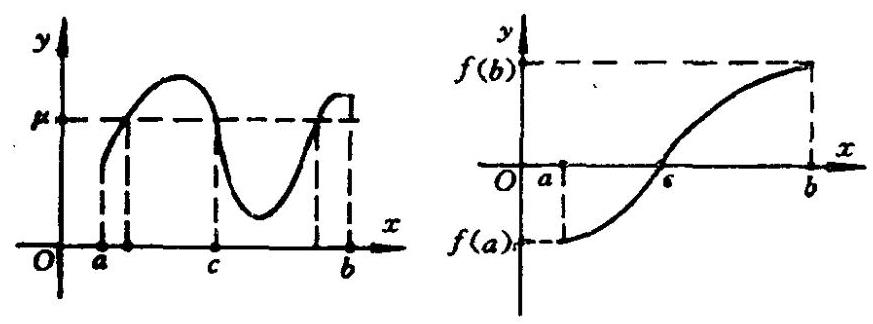
\includegraphics[max width=0.7\textwidth]{images/bo_d25ksc77aajc738obdgg_185_421_502_873_324_0.jpg}
\end{center}
\hspace*{3em} 

图 4-9

推论 2 设 $I \subset  \mathrm{R}$ 是任一区间, $f : I \rightarrow  \mathrm{R}$ 是任一连续函数,则 $f\left( I\right)$ 也是一个区间.

证明 根据第 3 章 § 4 习题 10 的结论, 我们只需证明:
$$\forall {y}_{1},{y}_{2} \in  f\left( I\right) \text{ 且 }{y}_{1} < {y}_{2} \Rightarrow  \left\lbrack  {{y}_{1},{y}_{2}}\right\rbrack   \subset  f\left( I\right) \text{ . }$$

令 ${x}_{1},{x}_{2} \in  I$ ,使 ${y}_{1} = f\left( {x}_{1}\right) ,{y}_{2} = f\left( {x}_{2}\right)$ . 不妨设 ${x}_{1} < {x}_{2}$ . 于是由上述定理知,
$$\left\lbrack  {{y}_{1},{y}_{2}}\right\rbrack   \subset  \left\lbrack  {\mathop{\inf }\limits_{{x \in  {x}_{1},{x}_{2}}}f\left( x\right) ,\mathop{\sup }\limits_{{x \in  {x}_{1},{x}_{2}}}f\left( x\right) }\right\rbrack   = f\left( \left\lbrack  {{x}_{1},{x}_{2}}\right\rbrack  \right)  \subset  f\left( I\right) .$$

例5 任意一个实系数的奇次代数方程
$${a}_{{2n} + 1}{x}^{{2n} + 1} + {a}_{2n}{x}^{2n} + \cdots  + {a}_{1}x + {a}_{0} = 0\;\left( {{a}_{{2n} + 1} \neq  0}\right)$$

至少有一个实根.

事实上,定义函数 $f : \mathbf{R} \rightarrow  \mathbf{R}$ 如下:
\begin{align*}
	&f\left( x\right)  = {a}_{{2n} + 1}{x}^{{2n} + 1} + {a}_{2n}{x}^{2n} + \cdots  + {a}_{1}x + {a}_{0}\;x \in  \mathbf{R}\\
	&= {a}_{{2n} + 1}{x}^{{2n} + 1}\left( {1 + \frac{{a}_{2n}}{{a}_{{2n} + 1}} \cdot  \frac{1}{x} + \cdots  + \frac{{a}_{1}}{{a}_{{2n} + 1}} \cdot  \frac{1}{{x}^{2n}}}\right.\\
	&\left. {+\frac{{a}_{0}}{{x}^{{2n} + 1}}}\right) \text{ . }
\end{align*}

右边括号内的表达式当 $\left| x\right|$ 充分大以后恒为正值,因此存在 $M >$ 0,使得 $f\left( M\right)$ 与 ${a}_{{2n} + 1}{M}^{{2n} + 1}$ 同号, $f\left( {-M}\right)$ 与 $- {a}_{{2n} + 1}{M}^{{2n} + 1}$ 同号,从而 $f\left( M\right)  \cdot  f\left( {-M}\right)  < 0$ . 由于 $f$ 在 $\left\lbrack  {-M,M}\right\rbrack$ 上连续,故由上述推论 1 知,至少存在一点 $c \in  \rbrack  - M,M\lbrack$ 使得 $f\left( c\right)  = 0$ .

\section*{3. 一致连续性}

设 $X \subset  \mathbf{R}$ 是任一非空集合, $f : X \rightarrow  \mathbf{R}$ 在 $X$ 上连续. 于是 $\forall {x}_{0} \in  X$ ,由连续性定义知
\begin{align*}
	&\left( {\forall \varepsilon  > 0}\right) \left( {\exists {\delta }_{{x}_{0}} > 0}\right) \left( {\forall x \in  X,\left| {x - {x}_{0}}\right|  < {\delta }_{{x}_{0}}}\right)\\
	&\Rightarrow  \left| {f\left( x\right)  - f\left( {x}_{0}\right) }\right|  < \varepsilon \text{ . }
\end{align*}

这里 ${\delta }_{{x}_{0}}$ 与 ${x}_{0}$ 有关,

如果 $\delta  = \mathop{\inf }\limits_{{{x}_{0} \in  X}}{\delta }_{{x}_{0}} > 0$ ,则显然我们有:
$$\forall x,{x}^{\prime } \in  X,\left| {x - {x}^{\prime }}\right|  < \delta  \Rightarrow  \left| {f\left( x\right)  - f\left( {x}^{\prime }\right) }\right|  < \bar{\varepsilon }.$$

但一般说来,可能出现 $\mathop{\inf }\limits_{{{x}_{0} \in  X}}{\delta }_{{x}_{0}} = 0$ 的情形.

例如考虑函数 $f : \rbrack 0,1\rbrack  \rightarrow  \mathbf{R}$ :
$$\forall x \in  \rbrack 0,1\rbrack ,f\left( x\right)  = \frac{1}{x}.$$

$\left. {\forall {x}_{0} \in  \rbrack 0,1}\right\rbrack  ,\forall x \in  \left\lbrack  {\frac{{x}_{0}}{2},1}\right\rbrack$ ,我们有
$$\left| {\frac{1}{x} - \frac{1}{{x}_{0}}}\right|  = \frac{\left| x - {x}_{0}\right| }{x{x}_{0}} < \frac{2\left| {x - {x}_{0}}\right| }{{x}_{0}^{2}}.$$

$\forall \varepsilon  > 0$ ,由 $\frac{2\left| {x - {x}_{0}}\right| }{{x}_{0}^{2}} < \varepsilon$ 得到 $\left| {x - {x}_{0}}\right|  < \frac{\varepsilon {x}_{0}^{2}}{2}$ . 若令

${\delta }_{{x}_{0}} = \frac{{x}_{0}^{2}\varepsilon }{2}$ ,则 ${\delta }_{{x}_{0}} > 0$ ,于是对 $0 < \bar{\varepsilon } < 1$ ,我们有:
$$\forall x \in  \rbrack 0,1\rbrack ,\left| {x - {x}_{0}}\right|  < {\delta }_{{x}_{0}} \Rightarrow  \left| {\frac{1}{x} - \frac{1}{{x}_{0}}}\right|  < \bar{\varepsilon }.$$

很显然,这里 $\mathop{\inf }\limits_{{{x}_{0} \in  0,1}}{\delta }_{{x}_{0}} = \mathop{\inf }\limits_{{{x}_{0} \in  0,1}}\frac{{x}_{0}^{2}\varepsilon }{2} = 0$ ,换句话说,不存在 $\delta  > 0$ 使得
$$\left. {\forall x,{x}^{\prime } \in  \rbrack 0,1}\right\rbrack  ,\left| {x - {x}^{\prime }}\right|  < \delta  \Rightarrow  \left| {\frac{1}{x} - \frac{1}{{x}^{\prime }}}\right|  < \varepsilon .$$

为了研究这种 “一致性” $\delta$ 的存在性,我们引进一致连续性的下述定义.

定义 设 $X \subset  \mathbf{R}$ 是任一非空集合, $f : X \rightarrow  \mathbf{R}$ 是任一函数, 我们称 $f$ 在 $X$ 上是一致连续的,如果下述性质成立:
\begin{align*}
	&\left( {\forall \varepsilon  > 0}\right) \left( {\exists \delta  > 0}\right) \left( {\forall x,{x}^{\prime } \in  X,\left| {x - {x}^{\prime }}\right|  < \delta }\right)\\
	&\Rightarrow  \left| {f\left( x\right)  - f\left( {x}^{\prime }\right) }\right|  < \varepsilon \text{ . }
\end{align*}

下面的定理指出了一个一致连续函数类.

定理 $4 \cdot  6 \cdot  5$ 设 $X \subset  \mathbf{R}$ 是有界闭集,若函数 $f : X \rightarrow  \mathbf{R}$ 连续, 则 $f$ 是一致连续的.

证明 用反证法. 假设 $f$ 在 $X$ 上不一致连续. 则
\begin{align*}
	&\left( {\exists {\varepsilon }_{0} > 0}\right) \left( {\forall \delta  > 0}\right) \left( {\exists {x}^{\prime },{x}^{\prime \prime } \in  X,\left| {{x}^{\prime } - {x}^{\prime \prime }}\right|  < \delta }\right)\\
	&\Rightarrow  \left| {f\left( {x}^{\prime }\right)  - f\left( {x}^{\prime \prime }\right) }\right|  \geq  {\varepsilon }_{0}.
\end{align*}

取 $\delta  = \frac{1}{n}\left( {n \in  \mathbf{N}}\right)$ . 于是存在 ${x}_{n}^{\prime },{x}_{n}^{\prime \prime } \in  X$ 使得
$$\left| {{x}_{n}^{\prime } - {x}_{n}^{\prime \prime }}\right|  < \frac{1}{n},\left| {f\left( {x}_{n}^{\prime }\right)  - f\left( {x}_{n}^{\prime \prime }\right) }\right|  \geq  {\varepsilon }_{0}\;\left( {\forall n \in  \mathbf{N}}\right) .$$

由此得到两个实数序列 $\left\langle  {x}_{n}^{\prime }\right\rangle$ 与 $\left\langle  {x}_{n}^{\prime \prime }\right\rangle$ ,它们都是有界的. 由 Bolzano-Weierstrass定理知,序列 $\left\langle  {x}_{n}^{\prime }\right\rangle$ 有收敛子序列,不妨设 $\left\langle  {x}_{n}^{\prime }\right\rangle$ 本身收敛. 令 $\mathop{\lim }\limits_{{n \rightarrow   + \infty }}{x}_{n}^{\prime } = \bar{x}$ . 由于 $X$ 是闭集,故 $\bar{x} \in  X$ .

另一方面, 由
$$\left| {{x}_{n}^{\prime } - {x}_{n}^{\prime \prime }}\right|  < \frac{1}{n},{x}_{n}^{\prime \prime } = \left( {{x}_{n}^{\prime \prime } - {x}_{n}^{\prime }}\right)  + {x}_{n}^{\prime }\;\left( {\forall n \in  \mathbf{N}}\right)$$

知, $\mathop{\lim }\limits_{{n \rightarrow  \infty }}\left( {{x}_{n}^{\prime } - {x}_{n}^{\prime \prime }}\right)  = 0$ ,从而序列 $\left\langle  {x}_{n}^{\prime \prime }\right\rangle$ 收敛,并且
$$\mathop{\lim }\limits_{{n \rightarrow   + \infty }}{x}_{n}^{\prime \prime } = \mathop{\lim }\limits_{{n \rightarrow   + \infty }}\left( {{x}_{n}^{\prime \prime } - {x}_{n}^{\prime }}\right)  + \mathop{\lim }\limits_{{n \rightarrow   + \infty }}{x}_{n}^{\prime } = \bar{x}.$$

现在对不等式 $\left| {f\left( {x}_{n}^{\prime }\right)  - f\left( {x}_{n}^{\prime \prime }\right) }\right|  \geq  {\varepsilon }_{0}\left( {\forall n \in  \mathbf{N}}\right)$ 令 $n \rightarrow   + \infty$ 取极限,由 $f$ 的连续性推知
$${\varepsilon }_{0} \leq  \left| {\mathop{\lim }\limits_{{n \rightarrow  \infty }}f\left( {x}_{n}^{\prime }\right)  - \mathop{\lim }\limits_{{n \rightarrow   + }}f\left( {x}_{n}^{\prime \prime }\right) }\right|  = \left| {f\left( \bar{x}\right)  - f\left( \bar{x}\right) }\right|  = 0.$$

这与 ${\varepsilon }_{0} > 0$ 矛盾。

因此 $f$ 在 $X$ 上一致连续.

例6 正弦、余弦函数 $x \mapsto  \sin x,x \mapsto  \cos x,x \in  \mathbf{R}$ ,在 $\mathbf{R}$ 上一致连续.

事实上, $\forall x,{x}^{\prime } \in  \mathbf{R}$ ,我们有
$$\left| {\sin x - \sin {x}^{\prime }}\right|  = 2\left| {\sin \frac{x - {x}^{\prime }}{2}}\right| \left| {\cos \frac{x + {x}^{\prime }}{2}}\right|  \leq  \left| {x - {x}^{\prime }}\right| .$$

于是
\begin{align*}
	&\left( {\forall \varepsilon  > 0}\right) \left( {\exists \delta  = \varepsilon }\right) \left( {\forall x,{x}^{\prime } \in  \mathbf{R},\left| {x - {x}^{\prime }}\right|  < \delta }\right)\\
	&\Rightarrow  \left| {\sin x - \sin {x}^{\prime }}\right|  < \varepsilon \text{ . }
\end{align*}

因此正弦函数 $x \mapsto  \sin x,x \in  \mathbf{R}$ 在 $\mathbf{R}$ 上一致连续.

同理可证余弦函数 $x \mapsto  \cos x,x \in  \mathbf{R}$ 在 $\mathbf{R}$ 上一致连续.

例7 函数 $x \mapsto  \frac{1}{x},x \in  \left\rbrack  {0,1}\right\rbrack$ ,在 $\rbrack 0,1\rbrack$ 上不是一致连续的,但 $\forall 0 < a < 1$ ,此函数在 $\left\lbrack  {a,1}\right\rbrack$ 上是一致连续的.

由于 $\left\lbrack  {a,1}\right\rbrack$ 是有限闭区间,故由上述定理知,此函数在 $\left\lbrack  {a,1}\right\rbrack$ 上一致连续. 为了证明它在 $\rbrack 0,1\rbrack$ 上不一致连续. 令
$${x}_{n} = \frac{1}{2n},{x}_{n}^{\prime } = \frac{1}{n}\left( {\forall n \in  \mathbf{N}}\right) ,$$

则 $\left| {{x}_{n} - {x}_{n}^{\prime }}\right|  = \frac{1}{2n} \rightarrow  0\left( {n \rightarrow   + \infty }\right)$ ,但 $\left| {\frac{1}{{x}_{n}} - \frac{1}{{x}_{n}^{\prime }}}\right|  = n > 1$ .

此即表明此函数在 $\rbrack 0,1\rbrack$ 上不一致连续.

定理 $4 \cdot  6 \cdot  6$ 设 $X \subset  \mathbf{R}$ 是任一有界集, $f : X \rightarrow  \mathbf{R}$ 在 $X$ 上一致连续,则 $f$ 在 $X$ 上连续、有界.

证明 $f$ 的连续性是显然的. 假设 $f$ 在 $X$ 上无界. 那末
$$\left( {\forall n \in  \mathbf{N}}\right) \left( {\exists {x}_{n} \in  X}\right)  \Rightarrow  \left| {f\left( {x}_{n}\right) }\right|  > n.$$

由此得一实数序列 $\left\langle  {x}_{n}\right\rangle$ . 由 Bolzano-Weierstrass定理知, 不妨设 $\left\langle  {x}_{n}\right\rangle$ 本身收敛.

另一方面,由于 $f$ 在 $X$ 上一致连续,故由定义有:
\begin{align*}
	&\left( {\forall \varepsilon  > 0}\right) \left( {\exists \delta  > 0}\right) \left( {\forall x,{x}^{\prime } \in  X,\left| {x - {x}^{\prime }}\right|  < \delta }\right)\\
	&\Rightarrow  \left| {f\left( x\right)  - f\left( {x}^{\prime }\right) }\right|  < \varepsilon \text{ . }
\end{align*}

又因为 $\left\langle  {x}_{n}\right\rangle$ 收敛,所以 $\left\langle  {x}_{n}\right\rangle$ 是 Cauchy 序列,从而对上述 $\delta  > 0$ ,存在 $N \in  \mathbf{N}$ ,使得
$$\forall n,m \in  \mathbf{N},n,m \geq  N \Rightarrow  \left| {{x}_{n} - {x}_{m}}\right|  < \delta .$$

由此得到
$$\forall n,m \in  \mathbf{N},n,m \geq  N \Rightarrow  \left| {f\left( {x}_{n}\right)  - f\left( {x}_{m}\right) }\right|  < \bar{\varepsilon }.$$

此即表明 $\left\langle  {f\left( {x}_{n}\right) }\right\rangle$ 是 Cauchy 实数序列. 从而序列 $\left\langle  {f\left( {x}_{n}\right) }\right\rangle$ 有界, 这显然与前面的不等式 $\left| {f\left( {x}_{n}\right) }\right|  > n\left( {\forall x \in  \mathbf{N}}\right)$ 相矛盾. 因此 $f$ 在 $X$ 上有界.

现在我们用此定理来重新证明例7的函数 $x \mapsto  \frac{1}{x},x \in  \rbrack 0,1\rbrack$ , 在 $\rbrack 0,1\rbrack$ 上不一致连续就十分简单,因为此函数在 $\rbrack 0,1\rbrack$ 上无界.

定理 $4 \cdot  6 \cdot  6$ 的逆命题不成立.

例 8 函数 $x \rightarrow  \sin  - \frac{1}{x},x \in  \rbrack 0,1\rbrack$ ,在 $\rbrack 0,1\rbrack$ 上有界,并且连续, 但不一致连续.

事实上,对 ${\varepsilon }_{0} = 1$ ,及 $\forall \delta  > 0,\exists n \in  \mathbf{N}$ 使得
$${x}^{\prime } = \frac{1}{2n\pi },{x}^{\prime \prime } = \frac{1}{{2n\pi } + \frac{\pi }{2}} \in  \rbrack 0,1\rbrack \text{ 且 }\left| {{x}^{\prime } - {x}^{\prime \prime }}\right|  < \delta .$$

但是
$$\left| {\sin \frac{1}{{x}^{\prime }} - \sin \frac{1}{{x}^{\prime \prime }}}\right|  = \left| {\sin {2n\pi } - \sin \left( {{2n\pi } + \frac{\pi }{2}}\right) }\right|  = 1.$$

\section*{习 题}

1. 设 $f,g : \rbrack a,b\lbrack  \rightarrow  R$ 是任意两个连续函数.

1) 证明: $E = \{ x \in  \rbrack a,b\left\lbrack  {\mid f\left( x\right)  = 0}\right. \}$ 是开集.

2) 证明: $F = \{ x \in  \rbrack a,b\left\lbrack  {\mid f\left( x\right)  > g\left( x\right) }\right\}$ 是开集.

3) 证明: $G = \{ x \in  \rbrack a,b\left\lbrack  {\mid f\left( x\right)  = g\left( x\right) }\right\rbrack$ 是闭集.

2. 设连续函数 $f,g : \left\lbrack  {a,b}\right\rbrack   \rightarrow  \mathrm{R}$ 满足不等式
$$0 < g\left( x\right)  < f\left( x\right) ,\;\forall x \in  \left\lbrack  {a,b}\right\rbrack  .$$

证明: 存在 $k > 1$ 使得 ${kg}\left( x\right)  \leq  f\left( x\right) ,\forall x \in  \left\lbrack  {a,b}\right\rbrack$ .

3. 设连续函数 $f,g : \left\lbrack  {0,1}\right\rbrack   \rightarrow  R$ 满足条件
$$f\left( 0\right)  = 0,f\left( 1\right)  = 1,g\left( 0\right)  = 1,g\left( 1\right)  = 0.$$

证明: $\forall \lambda  \in  {\mathbf{R}}^{ + },\exists x \in  \left\lbrack  {0,1}\right\rbrack$ 使得 $f\left( x\right)  = {\lambda g}\left( x\right)$ .

4. 设 $f,g : \left\lbrack  {a,b}\right\rbrack   \rightarrow  \left\lbrack  {a,b}\right\rbrack$ 是任意两个连续函数.

1) 证明: 至少存在一个 ${x}_{0} \in  \left\lbrack  {a,b}\right\rbrack$ ,使得 $f\left( {x}_{0}\right)  = {x}_{0}$ .

2) 若 $f \circ  g = g \circ  f$ ,则至少存在一个 ${x}_{0} \in  \left\lbrack  {a,b}\right\rbrack$ 使得 $f\left( {x}_{0}\right)  = g\left( {x}_{0}\right)$ .

5. 设 $I \subset  R$ 是任一区间, $f : I \rightarrow  R$ 是任一函数.

1) 证明: 若 $f$ 在 $I$ 上连续,并且 $f\left( I\right)  \subset  Q$ ,则 $f$ 是常值函数.

2) 证明: 若 $f$ 在 $I$ 上连续,并且 $f\left( I\right)  \subset  {\mathbf{Q}}^{c}$ ,则 $f$ 是常值函数.

3) 证明: 若 $I$ 不为单元集,并且 $f\left( {I \cap  Q}\right)  \subset  {Q}^{c},f\left( {I \cap  {Q}^{c}}\right)  \subset  Q$ ,则 $f$ 在 $I$ 上不可能连续.

6. 设连续函数 $f,g : \left\lbrack  {a,b}\right\rbrack   \rightarrow  R$ 满足条件:
$$f\left( x\right)  = 0,\;{f}^{2}\left( x\right)  = {g}^{2}\left( x\right) ,\;\forall x \in  \left\lbrack  {a,b}\right\rbrack  .$$

证明: 下述两种情形中有且只有一种情形出现:

1) $f\left( x\right)  = g\left( x\right) ,\forall x \in  \left\lbrack  {a,b}\right\rbrack  ;2)f\left( x\right)  =  - g\left( x\right) ,\forall x \in  \left\lbrack  {a,b}\right\rbrack$ .

7. 设 $a \in  R,f : \lbrack a, + \infty \lbrack  \rightarrow  R$ 是任一连续函数. 并且 $\mathop{\lim }\limits_{{x \rightarrow   + \infty }}f\left( x\right)  = A$ (有限或 $\pm  \infty$ )

1) 证明: $f$ 取介于 $f\left( a\right)$ 与 $A$ 之间的一切值.

2) 证明: 若 $A =  + \infty$ ,则 $f$ 是下有界的,并且 $f$ 达到它的下确界.

8. 设 ${P}_{n}\left( x\right)  = {x}^{n} + {a}_{n - 1}{x}^{n - 1} + \cdots  + {a}_{1}x + {a}_{0}$ . 证明:

1) 若 ${a}_{0} < 0$ ,则 ${P}_{n}\left( x\right)  = 0$ 至少有一个正根。

2) 若 ${a}_{0} < 0$ ,且 $n$ 为偶数,则 ${P}_{n}\left( x\right)  = 0$ 至少有一个负根.

3) 若 $n$ 为偶数,则存在 $\bar{x} \in  \mathrm{R}$ 使得 ${P}_{n}\left( x\right)  \geq  {P}_{n}\left( \bar{x}\right) \forall x \in  \mathrm{R}$ . 由此推出: 存在实数 $m$ 使得 $\forall b \geq  m$ ,方程 ${P}_{n}\left( x\right)  = b$ 有实解存在,而 $\forall b < m$ , 方程 ${P}_{n}\left( x\right)  = b$ 没有实解存在.

9. 设 $\left\lbrack  {a,b}\right\rbrack   \subset  R$ 是任一有限闭区间, $f : \left\lbrack  {a,b}\right\rbrack   \rightarrow  R$ 是任一连续函数.

1)令

$\mathcal{A} = \{ I \mid  I$ 是 $\left\lbrack  {a,b}\right\rbrack$ 的闭子区间使得 $f$ 在 $I$ 上有界 $\} .$

证明: $\mathcal{A}$ 是 $\left\lbrack  {a,b}\right\rbrack$ 的一个完全覆盖. 由此推出 $f$ 在 $\left\lbrack  {a,b}\right\rbrack$ 上有界.

2) 设在 $\left\lbrack  {a,b}\right\rbrack$ 上 $f \neq  0$ . 令

$\mathcal{B} = \{ I \mid  I$ 是 $\left\lbrack  {a,b}\right\rbrack$ 的闭子区间使 $f$ 在 $I$ 上不变号 $\}$ .

证明: $\mathcal{B}$ 是 $\left\lbrack  {a,b}\right\rbrack$ 的一个完全置盖. 由此推出:若 $f\left( a\right) f\left( b\right)  < 0$ ,则至少存在一点 $\xi  \in  \left\lbrack  {a,b}\right\rbrack$ 使得 $f\left( \xi \right)  = 0$ .

3) $\forall \varepsilon  > 0$ ,令

$\sigma  = \{ I \mid  I$ 是 $\left\lbrack  {a,b}\right\rbrack$ 的闭子区间,使得
$$\forall x,y \in  I,\left| {f\left( x\right)  - f\left( y\right) }\right|  < \{ \varepsilon /2\} .$$

证明: $e$ 是 $\left\lbrack  {a,b}\right\rbrack$ 的一个完全覆盖,由此推出 $f$ 在 $\left\lbrack  {a,b}\right\rbrack$ 上一致连续.

10. 直接用定义证明: 函数 $x \mapsto  \sqrt{x},x \in  \lbrack 0, + \infty \lbrack$ ,在 $\left\lbrack  {0,1}\right\rbrack$ 上一致连续.

11. 证明: 函数 $x \mapsto  {x}^{2}$ 在 $x \in  \left\lbrack  {0,a}\right\rbrack$ 上一致连续,但在 $\lbrack 0, + \infty \lbrack$ 上不一致连续 (这里 $a > 0$ ).

12. 证明: 函数 $x \rightarrow  \sin {x}^{2},x \in  R$ ,在 $R$ 上不一致连续.

13. 设函数 $f : \left\lbrack  {a, + \infty \left\lbrack  { \rightarrow  \mathrm{R}}\right. }\right.$ 在 $\lbrack a, + \infty \lbrack$ 上连续,并且 $\mathop{\lim }\limits_{{x \rightarrow   + \infty }}f\left( x\right)  = A \in$ R. 证明: $f$ 在 $\lbrack a, + \infty \lbrack$ 上一致连续.

14. 设 $X \subset  R$ 是任一闭集. $f : X \rightarrow  R$ 是任一单调的有界连续函数. 证明: $f$ 在 $X$ 上一致连续.

15. 设 $X \subset  R$ 是任一非空集合, $f : X \rightarrow  R$ 是任一函数, $a \in  X$ 是 $X$ 的一个聚点. 我们称 $f$ 在 $a$ 处是上(下)半连续的,如果下述性质成立:
\begin{align*}
	&\forall \lambda  > f\left( a\right) \left( {\lambda  < f\left( a\right) }\right) ,\exists \delta  > 0,\forall x \in  X \cap  B\left( {a,\delta }\right)\\
	&\Rightarrow  \lambda  > f\left( x\right) \left( {\lambda  < f\left( x\right) }\right) .
\end{align*}

1) 证明: $f$ 在 $a$ 处下半连续的充分必要条件是函数 $- f$ 在 $a$ 处是上半连续的.

2)证明: $f$ 在 $a$ 处连续当且仅当 $f$ 在 $a$ 处既上半连续,又下半连续.

3) 证明: Dirichlet函数
$$x \mapsto  D\left( x\right)  = \left\{  \begin{array}{ll} 1, & x \in  \mathbf{Q}; \\  0, & x \in  {\mathbf{Q}}^{c}, \end{array}\right.$$

在任一有理点 $a$ 处是上半连续的,而在任一无理点 $a$ 处是下半连续的.

4 )考 虑函数
$$x \mapsto  f\left( x\right)  = \left\{  {\begin{array}{ll} 0, & x = 0; \\  \frac{1}{{x}^{k}}, & x \neq  0, \end{array}\left( {k \in  N}\right) .}\right.$$

证明: 若 $k$ 是偶数时, $f$ 在 0 处是下半连续的,若 $k$ 是奇数时, $f$ 在 0 处既不是上半连续的, 又不是下半连续的.

5) 证明: $f$ 在 $a$ 处下半连续当且仅当 $f\left( a\right)  = \mathop{\lim }\limits_{{x \rightarrow  a}}f\left( x\right)$ .

6) 设 $X \subset  R$ 是任一开区间. 则 $f$ 在 $X$ 上是下半连续 (即 $\forall a \in  X,f$ 在 $a$ 处下半连续) 当且仅当 $\forall \lambda  \in  \mathrm{R}$ ,集合 $\{ x \in  X \mid  f\left( x\right)  > \lambda \}$ 是开集.

7) 设 $A \subset  R$ 是任一集合,证明 $A$ 是开集当且仅当 $A$ 的特征函数 ${x}_{A}$ 在 $R$ 上是下半连续的,而 $A$ 是闭集当且仅当 ${\chi }_{A}$ 在 $R$ 上是上半连续的.

\section{单调连续函数的反函数}

\section*{1. 反函数存在性}

定理 $4 \cdot  7 \cdot  1$ 设 $I \subset  \mathbf{R}$ 是任一非空区间, $f : I \rightarrow  \mathbf{R}$ 是任一严格单调上升 (下降) 的连续函数. 则

1) $f : I \rightarrow  f\left( I\right)$ 是一一映射.

2) $f$ 的逆映射 ${f}^{-1} : f\left( I\right)  \rightarrow  I$ 也是严格单调上升 (下降) 的连续函数 $\left( {f}^{-1}\right.$ 通常称为 $f$ 的反函数).

证明 我们假设 $f$ 是严格单调上升的. 对严格单调下降的情形可类似证明.

1) 因为 $f$ 是严格单调上升的,所以 $f$ 是单射,从而 $f : I \rightarrow$  $f\left( I\right)$ 是一一映射. 因此 $f$ 的逆映射 ${f}^{-1} : f\left( I\right)  \rightarrow  I$ 存在.

2) 设 ${y}_{1},{y}_{2} \in  f\left( I\right)$ 且 ${y}_{1} < {y}_{2}$ . 若 ${f}^{-1}\left( {y}_{1}\right)  \geq  {f}^{-1}\left( {y}_{2}\right)$ ,则由 $f$ 的严格单调上升性及 $f \circ  {f}^{-1} = i{d}_{J}\left( I\right)$ 知
$${y}_{1} = f \circ  {f}^{-1}\left( {y}_{1}\right)  \geq  f \circ  {f}^{-1}\left( {y}_{2}\right)  = {y}_{2},$$

这与假设相矛盾. 因此 ${f}^{-1}\left( {y}_{1}\right)  < {f}^{-1}\left( {y}_{2}\right)$ ,即 ${f}^{-1}$ 是严格单调上升函数.

下面证明 ${f}^{-1}$ 在 $f\left( I\right)$ 上连续. 任取 ${y}_{0} \in  f\left( I\right)$ .

由于 $I$ 是区间,故 $f\left( I\right)$ 也是一个区间.

1) ${y}_{0} \in  f\left( \overset{ \circ  }{I}\right)$ : 于是 ${f}^{-1}\left( {y}_{0}^{ - }\right) ,{f}^{-1}\left( {y}_{0}^{ - }\right)$ 存在. 为了证明 ${f}^{-1}$ 在 ${y}_{0}$ 处连续,我们只需证明 ${f}^{-1}\left( {y}_{0}^{ - }\right)  = {f}^{-1}\left( {y}_{0}^{ - }\right)  = f\left( {y}_{0}^{ - }\right)$ .

首先由 ${f}^{-1}$ 的单调上升性,我们有:
\begin{align*}
	&\forall y \in  f\left( I\right) \text{ 且 }y < {y}_{0},{f}^{-1}\left( y\right)  < {f}^{-1}\left( {y}_{0}^{ - }\right) ,\\
	&\forall y \in  f\left( I\right) \text{ 且 }{y}_{0} < y,{f}^{-1}\left( {y}_{0}^{ - }\right)  < f\left( y\right) .
\end{align*}

因此
\begin{align*}
	&\left. {{f}^{-1}\left( {\rbrack  - \infty ,{y}_{0}\left\lbrack  {\mid f\left( I\right) }\right\rbrack   \subset  \rbrack  - \infty ,{f}^{-1}\left( {y}_{0}^{ - }\right) }\right) }\right\rbrack  \text{ , }\\
	&{f}^{-1}\left( {\rbrack {y}_{0}, + \infty \lbrack }\right) \left\lbrack  {f\left( I\right) }\right\rbrack   \subset  \left\lbrack  {{f}^{-1}\left( {y}_{0}^{ + }\right) , + \infty \lbrack }\right. \text{ . }
\end{align*}

从而
\begin{align*}
	&I = {f}^{-1}\left( {f\left( I\right) }\right)\\
	&= {f}^{-1}\left( {\left( {\rbrack  - \infty ,{y}_{0}\lbrack  \cap  f\left( I\right) }\right) \cup \{ {y}_{0}\} \cup (\rbrack {y}_{0}, + \infty \lbrack  \cap  f\left( I\right) }\right) )\\
	&= {f}^{-1}\left( {\rbrack  - \infty ,{y}_{0}\lbrack }\right)  \cap  f\left( I\right) ) \cup  {f}^{-1}\left( {y}_{0}\right)\\
	&\cup  {f}^{-1}\left( {\rbrack {y}_{0}, + \infty \lbrack }\right)  \cap  f\left( I\right) )\\
	&\subset  \rbrack  - \infty ,{f}^{-1}\left( {y}_{0}^{ - }\right) \rbrack  \cup  {f}^{-1}\left( {y}_{0}^{ - }\right)  \cup  \left\lbrack  {{f}^{-1}\left( {y}_{0}^{ + }\right) , + \infty \lbrack }\right. \text{ . }
\end{align*}

因为 $I$ 是一个区间,并且 ${f}^{-1}\left( {y}_{0}^{ - }\right)  \leq  {f}^{-1}\left( {y}_{0}^{ - }\right)  \leq  {f}^{-1}\left( {y}_{0}^{ + }\right)$ ,所以必然有 ${f}^{-1}\left( {y}_{0}^{ - }\right)  = {f}^{-1}\left( {y}_{0}\right)  = {f}^{-1}\left( {y}_{0}^{ + }\right)$ .

2) ${y}_{0} = \inf f\left( I\right)$ : 则 ${f}^{-1}\left( {y}_{0}\right)  \leq  {f}^{-1}\left( {y}_{0}^{ + }\right)$ . 由于
\begin{align*}
	&I = {f}^{-1}\left( {f\left( I\right) }\right)\\
	&= {f}^{-1}\left( {\left\{  {y}_{0}\right\}   \cup  \left( {\rbrack {y}_{0}, + \infty \lbrack  \cap  f\left( I\right) }\right) }\right)\\
	&\subset  {f}^{-1}\left( {y}_{0}\right)  \cup  \left\lbrack  {{f}^{-1}\left( {y}_{0}^{ + }\right) , + \infty \lbrack }\right. \text{ . }
\end{align*}

故 ${f}^{-1}\left( {y}_{0}\right)  = {f}^{-1}\left( {y}_{0}^{ + }\right)$ . 因此 ${f}^{-1}$ 在 ${y}_{0}$ 处右连续.

3) ${y}_{0} = \sup f\left( I\right)$ : 则 ${f}^{-1}\left( {y}_{0}^{ - }\right)  \leq  {f}^{-1}\left( {y}_{0}\right)$ . 由于
\begin{align*}
	&I = {f}^{-1}\left( {f\left( I\right) }\right)\\
	&= {f}^{-1}\left( {\left( {\rbrack  - \infty ,{y}_{0}\lbrack  \cap  f\left( I\right) }\right) \cup \{ {y}_{0}\} }\right)\\
	&\subset  \rbrack  - \infty ,{f}^{-1}\left( {y}_{0}\right) \rbrack  \cup  {f}^{-1}\left( {y}_{0}\right) \text{ , }
\end{align*}

因此 ${f}^{-1}\left( {y}_{0}^{ - }\right)  = {f}^{-1}\left( {y}_{0}\right)$ . 即 $f$ 在 ${y}_{0}$ 处左连续.

\section*{2. 函数 $f$ 的图形与反函数 ${f}^{-1}$ 的图形}

根据函数图形的定义我们有
\begin{align*}
	&\operatorname{Gr}\left( f\right)  = \{ \left( {x,f\left( x\right) }\right)  \mid  x \in  I\} ,\\
	&\operatorname{Gr}\left( {f}^{-1}\right)  = \left\{  {\left( {y,{f}^{-1}\left( y\right) }\right)  \mid  y \in  f\left( I\right) }\right\}  .
\end{align*}

$\forall y \in  f\left( I\right)$ ,令 $x \in  I$ 使得 $y = f\left( x\right)$ ,则 ${f}^{-1}\left( y\right)  = {f}^{-1}\left( {f\left( x\right) }\right)  = x$ , 因此
$$\operatorname{Gr}\left( {f}^{-1}\right)  = \{ \left( {f\left( x\right) ,x}\right)  \mid  x \in  I\} .$$

由于在平面直角坐标系 $\{ 0;x,y\}$ 中点 $\left( {x,f\left( x\right) }\right)$ 与点 $\left( {f\left( x\right) ,x}\right)$ 关于直线 $y = x$ 对称,故在同一直角坐标系 $\{ 0;x,y\}$ 下, $\operatorname{Gr}\left( f\right)$ 与 $\operatorname{Gr}\left( {f}^{-1}\right)$ 关于直线 $y = x$ 对称 (图 4-10).

\begin{center}
	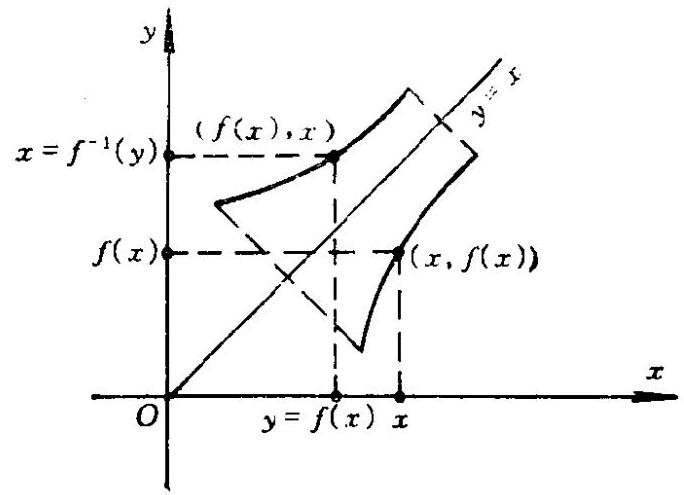
\includegraphics[max width=0.6\textwidth]{images/bo_d25ksc77aajc738obdgg_194_373_661_684_495_0.jpg}
\end{center}
\hspace*{3em} 

图 4-10

\section*{3. 三角函数的反函数}

1) 由于正弦函数 $\sin$ 在 $\left\lbrack  {-\frac{\pi }{2},\frac{\pi }{2}}\right\rbrack$ 上的限制 $x \mapsto  \sin x,x \in$  $\left\lbrack  {-\frac{\pi }{2},\frac{\pi }{2}}\right\rbrack$ 是严格单调上升的连续函数,并且
$$\mathop{\lim }\limits_{{x \rightarrow   - \frac{\pi }{2}}}\sin x =  - 1,\mathop{\lim }\limits_{{x \rightarrow  \frac{\pi }{2}}}\sin x = 1.$$

故它有从 $\left\lbrack  {-1,1}\right\rbrack$ 到 $\left\lbrack  {-\frac{\pi }{2},\frac{\pi }{2}}\right\rbrack$ 上的严格上升的连续反函数. 我

\section*{们记这个反函数为}
$$x \mapsto  \arcsin x,x \in  \left\lbrack  {-1,1}\right\rbrack  .$$

2) 由于余弦函数 $\cos$ 在 $\left\lbrack  {0,\pi }\right\rbrack$ 上的限制 $x \mapsto  \cos x,x \in  \left\lbrack  {0,\pi }\right\rbrack$ 是严格单调下降的连续函数, 并且
$$\mathop{\lim }\limits_{{x \rightarrow  0}}\cos x = 1,\mathop{\lim }\limits_{{x \rightarrow  \pi }}\cos x =  - 1$$

\begin{center}
	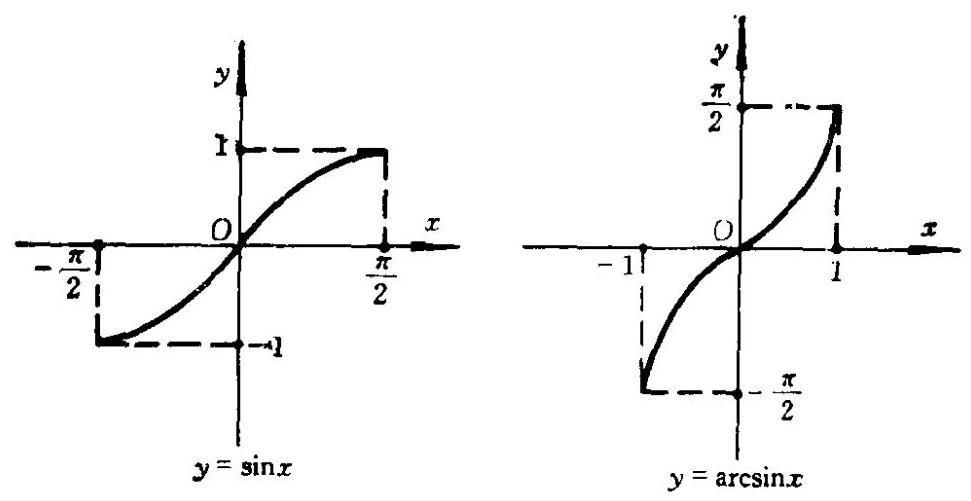
\includegraphics[max width=0.8\textwidth]{images/bo_d25ksc77aajc738obdgg_195_372_294_971_501_0.jpg}
\end{center}
\hspace*{3em} 

图 4-11

故它有从 $\left\lbrack  {-1,1}\right\rbrack$ 到 $\left\lbrack  {0,\pi }\right\rbrack$ 上的严格单调下降的连续反函数. 我们记这个反函数为
$$x \mapsto  \arccos x,x \in  \left\lbrack  {-1,1}\right\rbrack  .$$

\begin{center}
	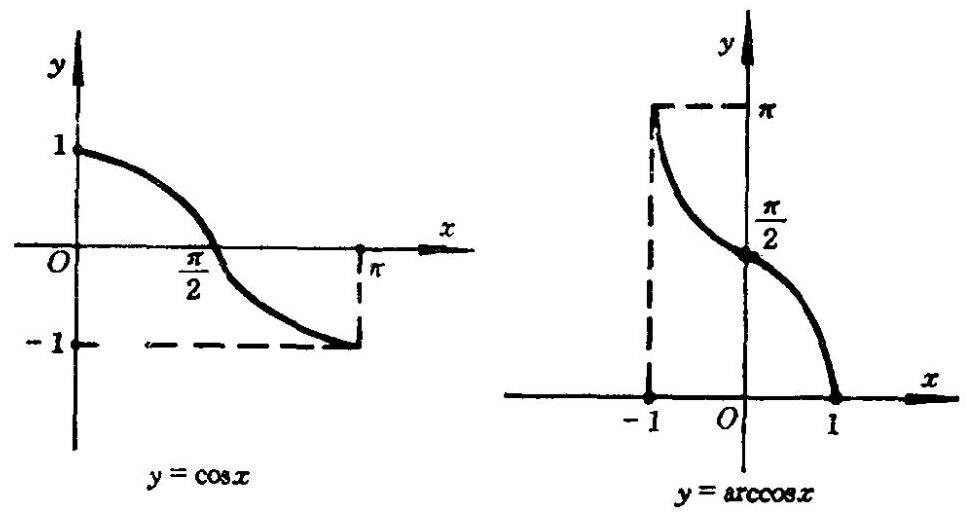
\includegraphics[max width=0.8\textwidth]{images/bo_d25ksc77aajc738obdgg_195_345_1203_967_519_0.jpg}
\end{center}
\hspace*{3em} 

图 4-12

3) 由于正切函数 $\operatorname{tg}$ 在 $\rbrack  - \frac{\pi }{2},\frac{\pi }{2}\lbrack$ 上的限制 $x \mapsto  \operatorname{tg}x,x \in$

$\left. {-\frac{\pi }{2},\frac{\pi }{2}}\right\rbrack$ . 是严格单调上升的连续函数,并且
$$\mathop{\lim }\limits_{{x \rightarrow   - \frac{{\pi }^{ + }}{2}}}\lg x =  - \infty ,\mathop{\lim }\limits_{{x \rightarrow  \frac{{\pi }^{ - }}{2}}}\lg x =  + \infty .$$

故它有从 $\rbrack  - \infty , + \infty \left\lbrack  \text{ 到 }\right\rbrack   - \frac{\pi }{2},\frac{\pi }{2}\lbrack$ 上的严格单调上升的连续反函数. 我们记这个反函数为
$$x \mapsto  \operatorname{arctg}x,x \in  \rbrack  - \infty , + \infty \lbrack \text{ . }$$

\begin{center}
	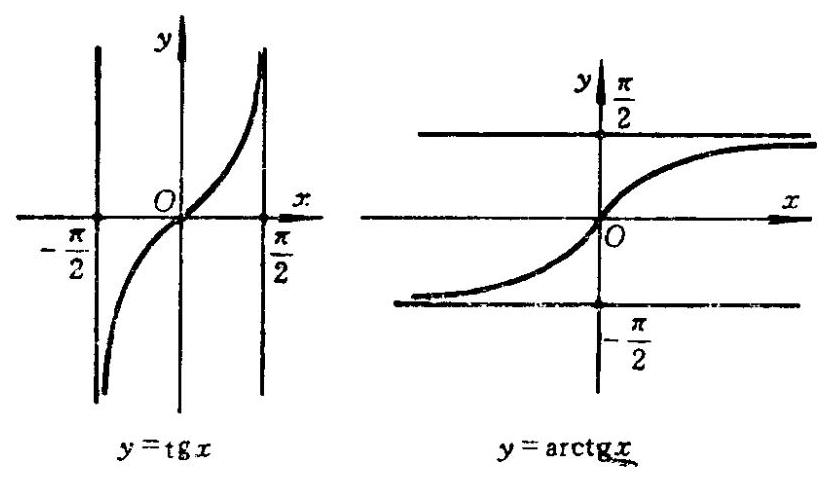
\includegraphics[max width=0.7\textwidth]{images/bo_d25ksc77aajc738obdgg_196_318_669_824_480_0.jpg}
\end{center}
\hspace*{3em} 

图 4-13

4) 由于余切函数 $\operatorname{ctg}$ 在 $\rbrack 0,\pi \lbrack$ 上的限制 $x \mapsto  \operatorname{ctg}x,x \in$

] $0,\pi \lbrack$ ,是严格单调下降的连续函数,并且
$$\mathop{\operatorname{limctg}}\limits_{{x \rightarrow  {0}^{ + }}}x =  + \infty ,\mathop{\operatorname{limctg}}\limits_{{x \rightarrow  {\pi }^{ - }}}x =  - \infty .$$

故它有从 $\rbrack  - \infty , + \infty \lbrack$ 到 $\rbrack 0,\pi \lbrack$ 上的严格单调下降的连续反函数. 我们记这个反函数为
$$x \mapsto  \operatorname{arcclg}x,x \in  \rbrack  - \infty , + \infty \lbrack \text{ . }$$

\begin{center}
	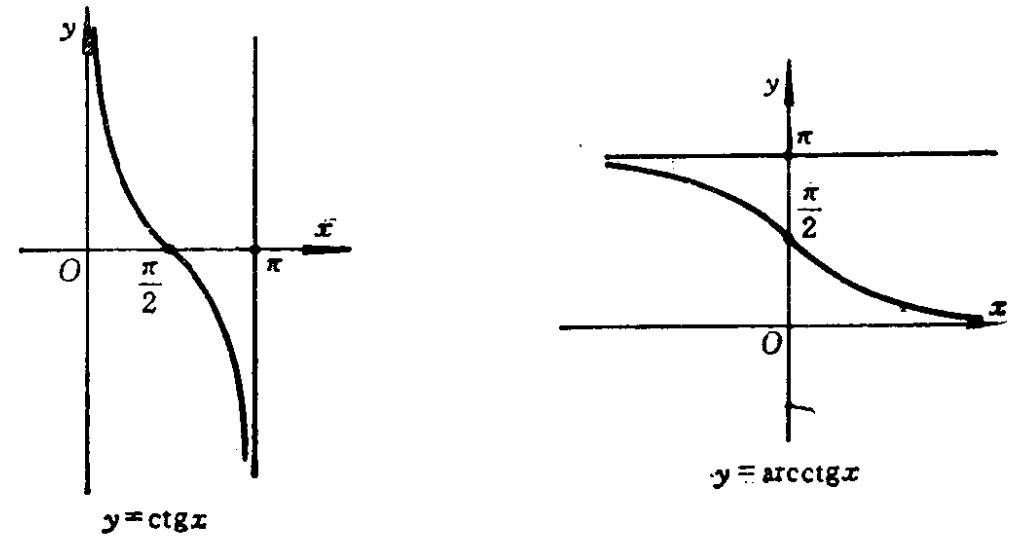
\includegraphics[max width=0.9\textwidth]{images/bo_d25ksc77aajc738obdgg_196_168_1520_1022_542_0.jpg}
\end{center}
\hspace*{3em} 

图 4-14

\section*{习 题}

1. 直接用 $\varepsilon  - \delta$ 语言证明定理 $4 \cdot  7 \cdot  1$ 中的反函数 ${f}^{-1} : f\left( I\right)  \rightarrow  I$ 的连续性.

2. 证明下列各等式:

1) $\arcsin \left( {-x}\right)  =  - \arcsin x,2)\arccos \left( {-x}\right)  = \pi  - \arccos x$ ,

3) $\operatorname{arctg}\left( {-x}\right)  =  - \operatorname{arctg}x,\;4)\operatorname{arcctg}\left( {-x}\right)  = \pi  - \operatorname{arcc}{gx}$ ,

5) $\arcsin x + \arccos x = \frac{\pi }{2}$ , 6) arctg $x + \operatorname{arcctg}x = \frac{\pi }{2}$ .

3. 考虑函数 $y \mapsto  f\left( y\right)  = y - \lambda \sin y,y \in  R\;\left( {0 \leq  \lambda  < 1}\right)$ .

1)证明: $f$ 是从 $R$ 到 $R$ 上的严格单调上升的连续函数.

2) 证明: 存在唯一的连续反函数 $x \mapsto  y\left( x\right) ,x \in  R$ ,满足方程
$$y - \lambda \sin y = x\;\left( {\forall x \in  R}\right) .$$

4. 设 $I \subset  R$ 是任一非空区间, $f : I \rightarrow  R$ 是任一单调函数,证明下述结论等价:

1) $f$ 在 $I$ 上连续. 2) $f\left( I\right)$ 是一区间.

5. 设 $I \subset  R$ 是任一非空区间, $f : I \rightarrow  R$ 是任一连续单射.

1) 证明: $\forall {x}_{1},{x}_{2} \in  I,{x}_{1} < {x}_{2},f$ 在 $\left\lbrack  {{x}_{1},{x}_{2}}\right\rbrack$ 上是单调的.

2) 由此推出 $f$ 在 $I$ 上是严格单调的.

